\documentclass[numsec,webpdf,modern,medium,namedate]{oup-authoring-template}

\onecolumn

%\usepackage{showframe}

\graphicspath{{Figures/}}

% line numbers
%\usepackage[mathlines, switch]{lineno}
%\usepackage[right]{lineno}

% Re-define OUP theorem styles with reduced spaceabove/below before declaring
% \newtheorem environments (same fix as main paper — see doubly_unlinked.tex).
\makeatletter
\newtheoremstyle{thmstyleone}%
  {3pt plus1pt minus1pt}%
  {3pt plus1pt minus1pt}%
  {\normalfont\itshape}%
  {0pt}%
  {\bfseries}%
  {}%
  {.5em}%
  {\thmname{#1}\thmnumber{\@ifnotempty{#1}{ }\@upn{#2}}\thmnote{ {\the\thm@notefont(#3)}}}%
\newtheoremstyle{thmstyletwo}%
  {3pt plus1pt minus1pt}%
  {3pt plus1pt minus1pt}%
  {\itshape}%
  {0pt}%
  {\normalfont}%
  {}%
  {.5em}%
  {\thmname{#1}\thmnumber{\@ifnotempty{#1}{ }{#2}}\thmnote{ {\the\thm@notefont(#3)}}}%
\newtheoremstyle{thmstylethree}%
  {3pt plus1pt minus1pt}%
  {3pt plus1pt minus1pt}%
  {\normalfont}%
  {0pt}%
  {\bfseries}%
  {}%
  {.5em}%
  {\thmname{#1}\thmnumber{\@ifnotempty{#1}{ }\@upn{#2}}\thmnote{ {\the\thm@notefont(#3)}}}%
\makeatother
\theoremstyle{thmstyleone}%
\newtheorem{theorem}{Theorem}%  meant for continuous numbers
%%\newtheorem{theorem}{Theorem}[section]% meant for sectionwise numbers
%% optional argument [theorem] produces theorem numbering sequence instead of independent numbers for Proposition
% \newtheorem{proposition}[theorem]{Proposition}%
\newtheorem{proposition}{Proposition}
\newtheorem{assumption}{Assumption}% to get separate numbers for theorem and proposition etc.
\theoremstyle{thmstyletwo}%
\newtheorem{example}{Example}%
\newtheorem{remark}{Remark}%
\theoremstyle{thmstylethree}%
\newtheorem{definition}{Definition}
\usepackage[doublespacing]{setspace}
\setdisplayskipstretch{1.0}
\usepackage{etoolbox}
\AtBeginDocument{%
  \setlength{\topsep}{6pt plus 1pt minus 1pt}%
}
% Reduce section/subsection pre-skip (same fix as main paper).
\makeatletter
\def\section{%
  \@startsection{section}{1}{\z@}
  {-4\p@ plus -2\p@}{\if@traditional\if@large.4\p@\else\if@medium6.5\p@\else4\p@\fi\fi\else\if@contemporary5\p@\else4\p@\fi\fi}
  {\reset@font\raggedright\secsize}}
\def\subsection{%
  \@startsection{subsection}{2}{\z@}
  {-4\p@ plus -2\p@}{\if@traditional.4\p@\else2\p@\fi}
  {\reset@font\raggedright\subsecsize}}
\makeatother
\usepackage[fontsize=12pt]{fontsize}

%%%%%%% CUSTOM PACKAGES %%%%%%%%%%
\usepackage{amsmath,amssymb,amsthm,mathrsfs,bm}
\DeclareMathOperator*{\argmax}{arg\,max}
\DeclareMathOperator*{\argmin}{arg\,min}
\newcommand{\noi}{\noindent}
\newcommand{\norm}[1]{\left\lVert #1 \right\rVert}
\newcommand{\nlim}{\xrightarrow[]{n \to \infty}}
\newcommand{\pnlim}{\xrightarrow[n \to \infty]{P}}
\newcommand{\klim}{\xrightarrow[]{k \to \infty}}
\newcommand{\aslim}{\xrightarrow[n \to \infty]{a.s.}}
\newcommand{\dnlim}{\xrightarrow[n \to \infty]{d}}
\newcommand{\lnlim}{\xrightarrow[n \to \infty]{L_2}}
\newcommand{\bmu}{\boldsymbol{\mu}}
\newcommand{\tr}{\mathrm{tr}}
\newcommand{\calB}{\mathcal{B}}
\newcommand{\calC}{\mathcal{C}}
\newcommand{\calD}{\mathcal{D}}
\newcommand{\calL}{\mathcal{L}}
\newcommand{\calP}{\mathcal{P}}
\newcommand{\calH}{\mathcal{H}}
\newcommand{\calHP}{\mathcal{P}}
\newcommand{\calI}{\mathcal{I}}
\newcommand{\calQ}{\mathcal{Q}}
\newcommand{\calN}{\mathcal{N}}
\newcommand{\R}{\mathbb{R}}
\newcommand{\N}{\mathbb{N}}
\newcommand{\Q}{\mathbb{Q}}
\newcommand{\bigo}{\mathcal{O}}
\newcommand{\smallo}{o}
\newcommand{\Z}{\mathbb{Z}}
\newcommand{\bdn}{\bar{d}_n}
\newcommand{\bE}{\mathbf{E}}
\newcommand{\bW}{\boldsymbol{W}}
\newcommand{\bX}{\boldsymbol{X}}
\newcommand{\bR}{\mathbf{R}}
\newcommand{\bpix}{\boldsymbol{\pi}_X}
\newcommand{\bpis}{\boldsymbol{\pi}_S}
\newcommand{\bPix}{\boldsymbol{\Pi}_X}
\newcommand{\bPis}{\boldsymbol{\Pi}_S}
\newcommand{\bPi}{\boldsymbol{\Pi}}
\newcommand{\bpi}{\boldsymbol{\pi}}
\newcommand{\hatpi}{\widehat{\boldsymbol{\pi}}}
\newcommand{\hatPi}{\widehat{\boldsymbol{\Pi}}}
\newcommand{\hatPix}{\widehat{\boldsymbol{\Pi}}_x}
\newcommand{\hatPis}{\widehat{\boldsymbol{\Pi}}_s}
\newcommand{\bPisx}{\boldsymbol{\Pi}_s\boldsymbol{\Pi}_x}
\newcommand{\delnu}{\Delta\nu}
\newcommand{\bY}{\boldsymbol{Y}}
\newcommand{\bM}{\mathbf{M}}
\newcommand{\bB}{\mathbf{B}}
\newcommand{\bK}{\mathbf{K}}
\newcommand{\by}{\boldsymbol{y}}
\newcommand{\bu}{\boldsymbol{u}}
\newcommand{\bz}{\boldsymbol{z}}
\newcommand{\bzet}{\boldsymbol{\zeta}}
\newcommand{\bGam}{\boldsymbol{\Gamma}}
\newcommand{\bQ}{\boldsymbol{Q}}
\newcommand{\bh}{\boldsymbol{h}}
\newcommand{\bD}{\boldsymbol{D}}
\newcommand{\bT}{\mathbf{T}}
\newcommand{\br}{\boldsymbol{r}}
\newcommand{\bV}{\mathbf{V}}
\newcommand{\bS}{\boldsymbol{S}}
\newcommand{\ba}{\boldsymbol{a}}
\newcommand{\balp}{\boldsymbol{\alpha}}
\newcommand{\snr}{\mathrm{SNR}}
\newcommand{\bdiag}{\mathrm{bdiag}}
\newcommand{\bDel}{\boldsymbol{\Delta}}
\newcommand{\bA}{\mathbf{A}}
\newcommand{\boldW}{\mathbb{W}}
\newcommand{\boldY}{\mathbb{Y}}
\newcommand{\boldX}{\mathbb{X}}
\newcommand{\boldM}{\mathbb{M}}
\newcommand{\boldV}{\mathbb{V}}
\newcommand{\bZ}{\boldsymbol{Z}}
\newcommand{\bU}{\boldsymbol{U}}
\newcommand{\bL}{\boldsymbol{L}}
\newcommand{\bP}{\mathbf{P}}
\newcommand{\bLam}{\boldsymbol{\Lambda}}
\newcommand{\blam}{\boldsymbol{\lambda}}
\newcommand{\bx}{\boldsymbol{x}}
\newcommand{\bI}{\mathbf{I}}
\newcommand{\beps}{\boldsymbol{\epsilon}}
\newcommand{\bet}{\boldsymbol{\eta}}
\newcommand{\bSig}{\boldsymbol{\Sigma}}
\newcommand{\Siginv}{\boldsymbol{\Sigma}^{-1}}
\newcommand{\ra}{\rightarrow}
\newcommand{\la}{\leftarrow}
\newcommand{\fld}{\mathcal{F}}
\newcommand{\Cov}{\text{Cov}\,}
\newcommand{\bard}{\bdn}
\newcommand{\pr}{\mathbb{P}}
\newcommand{\E}{\mathbb{E}}
\newcommand{\colsp}{\mathscr{C}}
% \newtheorem{theorem}{Theorem}
% \newtheorem{corollary}{Corollary}
% \newtheorem{lemma}{Lemma}
% \newtheorem{proposition}{Proposition}
% \newtheorem{posterior}{Posterior}
% \newtheorem{assumption}{Assumption}
% \theoremstyle{definition}
% \newtheorem{definition}{Definition}
% \newtheorem{remark}{Remark}
% \newtheorem{example}{Example}
% \newtheorem{conjecture}{Conjecture}
\newcommand{\Tau}{\mathcal{T}}
\newcommand{\bSigma}{{\boldsymbol{\Sigma}}}
\newcommand{\transpose}{^\top}
% %%%%%%%%%%%%%%%%%%%%%%%%%%%%%%%%%%%%%%%%%

\newcommand{\rough}{\underset{\sim}{<}}
\newcommand{\bH}{\boldsymbol{H}}
\newcommand{\bep}{\boldsymbol{\epsilon}}
\newcommand{\hbn}{\hat{\beta}_n}
\newcommand{\ets}{\eta^{*}}
% \newcommand{\BM}{\mathbf{M}}
\newcommand{\bTh}{\boldsymbol{\Theta}}
\newcommand{\bth}{\boldsymbol{\theta}}
\newcommand{\bets}{\boldsymbol{\eta}^{*}}
\newcommand{\betap}{\beta^{'}}
\newcommand{\ystbp}{Y^{*}_{\betap}}
\newcommand{\bystbp}{\boldsymbol{Y}^{*}_{\betap}}
\newcommand{\bystb}{\boldsymbol{Y}^{*}_{\beta}}
\newcommand{\Xstar}{X^{*}}
\newcommand{\bXstar}{\boldsymbol{X}^{*}}
\newcommand{\bs}{\boldsymbol{s}}
\newcommand{\tilX}{\widetilde{\boldsymbol{X}}}
\newcommand{\tilY}{\widetilde{\boldsymbol{Y}}}
\newcommand{\tbH}{\boldsymbol{H}^{'}}
\newcommand{\tbh}{\boldsymbol{h}^{'}}
\newcommand{\bdel}{\boldsymbol{\delta}}
\newcommand{\bnu}{\boldsymbol{\nu}}
\newcommand{\bgam}{\boldsymbol{\gamma}}
\newcommand{\bzero}{\boldsymbol{0}}
\newcommand{\Prob}{\mathbb{P}}
\newcommand{\Pst}{\mathbb{P}^{*}}
\newcommand{\betahat}{\hat{\beta}}

\newcommand{\hly}[1]{\colorbox{yellow}{#1}}
\newcommand{\iid}{\stackrel{\mathclap{\normalfont\tiny\mbox{iid}}}{\sim}}
\newcommand{\given}{\,|\,}
\newcommand{\biggiven}{\,\middle|\,}
\newcommand{\V}{\mathbb{V}}
\newcommand{\defeq}{\vcentcolon=}
\newcommand{\DY}{\mathrm{DY}}
\newcommand{\CM}{\mathrm{CM}}
\newcommand{\GCM}{\mathrm{GCM}}
\newcommand{\CMc}{\mathrm{CM_c}}
\newcommand{\GCMc}{\mathrm{GCM_c}}
\newcommand{\Cor}{\mathrm{Cor}}





% \newtheorem{theorem}{Theorem}
\newtheorem{corollary}{Corollary}
\newtheorem{lemma}{Lemma}
% \newtheorem{proposition}{Proposition}
% \newtheorem{posterior}{Posterior}
% \newtheorem{assumption}{Assumption}
% \newtheorem{definition}{Definition}
% \newtheorem{remark}{Remark}
% \newtheorem{example}{Example}
% \newtheorem{conjecture}{Conjecture}
\usepackage{mathtools}
\usepackage{nicefrac} 
\usepackage{hyperref}

\hypersetup{
    colorlinks=true,
    linkcolor=blue,      % internal links (sections, equations, figures)
    citecolor=blue,      % citation links
    urlcolor=blue        % URLs
}

% \captionsetup{compatibility=false}
\usepackage{xr-hyper}
\externaldocument{doubly_unlinked}

\begin{document}
% \spacingset{1.8}
\phantomsection\label{supplementary-material}
\bigskip
\begin{center}
{\large\bf Supplementary Materials for ``Doubly-Unlinked Regression for Dependent Data''}
\end{center}

\section{Details of Variational Inference}
Variational inference is a general approach for approximating a complicated target distribution by a simpler, tractable family of distributions. In Bayesian problems, the target is typically the posterior distribution of latent variables and model parameters given the observed data. When this posterior is analytically unavailable, direct computation is infeasible, and exact sampling-based methods may be computationally burdensome, variational inference replaces the original problem by an optimization problem. More specifically, one selects a family of candidate densities $\mathcal{Q}$ and then chooses the member $q^\ast \in \mathcal{Q}$ that is closest to the true posterior in Kullback--Leibler divergence. Equivalently, this can be formulated as maximizing the evidence lower bound (ELBO), which balances fidelity to the joint model with the entropy of the approximating distribution. The resulting approximation is often much faster to compute than Markov chain Monte Carlo, while still retaining a probabilistic characterization of uncertainty.

A particularly useful feature of variational inference is that it allows one to impose structural simplifications that make high-dimensional problems tractable. A common choice is the mean-field approximation, under which the variational density is factorized across groups of latent variables and parameters. This reduces posterior approximation to a sequence of lower-dimensional optimization steps, often yielding closed-form coordinate updates or efficient gradient-based optimization schemes. In models with latent Gaussian structure, conjugate priors, or exponential-family components, these updates can frequently be written explicitly, which leads to scalable inference even when the ambient dimension is large.

Variational inference is especially well suited to our framework because the doubly-unlinked regression problem introduces several latent objects simultaneously: the regression effect, the latent spatial process, covariance parameters, and two unknown permutation structures. The exact posterior over these quantities is highly coupled and combinatorial, since the permutations interact nonlinearly with both the regression and spatial dependence components. As a result, direct posterior computation is intractable, and naive enumeration over permutation configurations is impossible even for moderate block sizes. Variational inference provides a principled way to approximate this joint posterior while preserving the main dependence structure required for inference.

In our setting, variational inference serves two roles. First, it provides a computationally feasible mechanism for recovering the latent alignment structure induced by the unlinked observations. Second, it yields approximate posterior summaries for the scientific parameters of interest, including the regression coefficient and latent spatial surface, in a way that naturally propagates uncertainty from the unknown permutations. This is particularly important because the latent shuffling is not merely a nuisance computational feature; it is central to the statistical formulation of the problem. By combining a tractable variational family with blockwise structure, we obtain an inference procedure that is both scalable and well adapted to the privacy-preserving nature of the doubly-unlinked framework.
\subsection{Variational Density of Parameters}\label{appendix-vd-parameters}
As discussed in the Section \ref{sec:vb}, we assume a mean field approximation on the class of variational density of our target parameter vector. This provides a closed form solution to the densities which is given by the following theorem:
\begin{theorem}[\cite{ren2011variational}]\label{thm:optimal-vd}
     For a class of variational densities on $\bth = \left(\bth_1^\top,\cdots,\bth_k^\top\right)^\top$ given by the family $\calQ = \left\{q(\bth):q(\bth) = \prod_{l=1}^kq_l(\bth_i)\right\}$, the optimal $q^\ast_l(\bth_l)$ that maximizes the ELBO is given by:
    $$
    q^\ast_l(\bth_l) = \dfrac{\exp\{\E_{u \neq l}\log L(\mathbb{Y}_n,\bth|\mathbb{X}_n)\}}{\int \exp\{\E_{u \neq l}\log L(\mathbb{Y}_n,\bth|\mathbb{X}_n)\}\mathrm{d}\bth_l}
    $$
\end{theorem}

\textbf{Joint Likelihood.} The above theorem requires the computation of conditional joint likelihood $L(\mathbb{Y}_n,\bth\mid\mathbb{X}_n)$ for $n = KB$, which is given as:
\begin{equation}\label{eq:joint-likelihood}
    \begin{split}
&\log L(\mathbb{Y}_n,\bth\mid\mathbb{X}_n) \\
= & \log L(\mathbb{Y}_n\mid\bth,\mathbb{X}_n) + \log p(\bth)\\
= & - \frac{n}{2} \log2 \pi - \frac{n}{2}\log\tau^2-\frac{1}{2 \tau^2} \sum_{i=1}^B\left(\bY_i-\bpix \bX_i \beta -\bpis \bW_i\right)^{\top}\left(\bY_i-\bpix \bX_i \beta -\bpis \bW_i\right) \\
&- \frac{n}{2} \log 2 \pi-\frac{1}{2} \log |\bSig^\ast_n| - \frac{1}{2}\mathbb{W}_n^\top \bSig_n^{\ast-1} \mathbb{W}_n\\
& -\dfrac{1}{2}\log 2\pi\sigma^2_\beta-\dfrac{\beta^2}{2 \sigma_\beta^2}-C_\phi \\
&+a_1 \log b_1-\log \Gamma\left(a_1\right)-\left(a_1+1\right) \log \sigma^2 -\frac{b_1}{\sigma^2} \\
&+a_2 \log b_2-\log \Gamma\left(a_2\right)-\left(a_2+1\right) \log \tau^2 -\dfrac{b_2}{\tau^2}\\
&+\sum_{m=1}^{n}\sum_{k=1}^{n} \log \left[\frac{1}{\sqrt{2 \pi \eta^2_x}}\left\{\exp \left(-\frac{x_{m k}^2}{2 \eta_x^2}\right)+\exp \left(-\frac{\left(x_{m k}-1\right)^2}{2 \eta_x^2}\right)\right\}\right]\\
&+\sum_{m=1}^{n}\sum_{k=1}^{n}\log \left[\frac{1}{\sqrt{2 \pi \eta^2_s}}\left\{\exp \left(-\frac{s_{m k}^2}{2 \eta_s^2}\right)+\exp \left(-\frac{\left(s_{m k}-1\right)^2}{2 \eta_s^2}\right)\right\}\right]
    \end{split}
\end{equation}
Using Theorem~\ref{thm:optimal-vd}, we derive the optimal variational factors $q_l(\cdot)$ for the components of $\bth = (\mathbb{W}_n,\beta,\sigma^2,\phi,\tau^2,\bpix,\bpis)^\top$.
For each parameter \(\theta \in \bth\), the derivation proceeds by isolating all terms in the joint log-likelihood that depend on \(\theta\), while taking expectations with respect to the remaining variational factors. A key quantity in these updates is $\br_i \coloneq \bY_i - \bpix \bX_i \beta - \bpis \bW_i$, which denotes the residual term in the joint likelihood. In particular, for each \(\theta\), we compute the conditional expectation of \(\br_i^\top \br_i\) given \(\theta\), and combine it with the remaining $\theta$-dependent terms obtained after marginalizing over the other variables. This idea works only because of the mean filed approximation. Thus we start off by simplifying the quadratic term:
\begin{equation}\label{eq:residual-qf}
\begin{split}
    \br_i^\top \br_i &= (\bY_i - \bpix \bX_i \beta - \bpis \bW_i)^\top (\bY_i - \bpix \bX_i \beta - \bpis \bW_i) \\
&= \bY_i^\top \bY_i - 2 \bY_i^\top \bpix \bX_i \beta - 2 \bY_i^\top \bpis \bW_i \\
&\quad + \beta^2 \bX_i^\top \bpix^\top \bpix \bX_i \\
&\quad + 2 \beta \bX_i^\top \bpix^\top \bpis \bW_i \\
&\quad + \bW_i^\top \bpis^\top \bpis \bW_i 
\end{split}
\end{equation}
Recall from Section \ref{sec:vb} that $\E_{q_{\kappa_X}}[\bpix] = \bM^\ast_X$ and $\E_{q_{\kappa_X}}[\bpix^\top \bpix] = \bV^\ast_X$, while $\E_{q_{\kappa_S}}[\bpis] = \bM^\ast_S$ and $\E_{q_{\kappa_S}}[\bpis^\top \bpis] = \bV^\ast_S$. Another useful fact is that the dependence covariance matrix can always be written as $\bSig^\ast_n = \sigma^2 \bR(\phi)$. This decomposition will be used repeatedly in the derivations below, and in particular plays a central role in obtaining closed-form expressions for the parameters of the variational densities corresponding to our target quantities. 

\textbf{Variational density of $\beta$}
\begin{equation}\label{eq:residualsq-conditional-beta}
    \begin{split}
        \E_q[\br_i^\top \br_i \ |\ \beta]
        & = \bY_i^\top \bY_i - 2\beta \bX_i^\top {\bM^
        \ast_X}^\top \bY_i - 2 \bY_i^\top \bM^\ast_S \bmu_{W_i} \\
        &\quad + \beta^2 \bX_i^\top \bV^\ast_X \bX_i \\
        &\quad + 2 \beta \bX_i^\top {\bM^\ast_X}^\top \bM^\ast_S \bmu_{W_i} \\
        &\quad + \bmu_{W_i}^\top \bV^\ast_S \bmu_{W_i} + \text{tr}(\bV^\ast_S \bSig_{W_i})
    \end{split}
\end{equation}
Hence taking expectation over the joint likelihood in (\ref{eq:joint-likelihood}) except $\beta$, we have 
\begin{equation*}
    \begin{split}
        q_\beta(\beta) \propto & \exp\left(-\frac{1}{2} \E_{q_{\tau^2}}\left(\frac{1}{\tau^2}\right) \sum_{i=1}^B \E_q[\br_i^\top \br_i | \beta] - \frac{\beta^2}{2 \sigma^2_{\beta}}\right)\\
        = & \exp\left(-\frac{1}{2} \frac{\lambda_{a_2}}{\lambda_{b_2}} \sum_{i=1}^B \E_q[\br_i^\top \br_i | \beta] - \frac{\beta^2}{2 \sigma^2_{\beta}}\right)
    \end{split}
\end{equation*}
We will use this trick for the following parameters without explicitly mentioning it. This shows that the variational distribution of 
$\beta \sim \calN\left(\mu_{\lambda, \beta}, \sigma^2_{\lambda, \beta}\right)$ where the variational mean and variance are given by:
\begin{equation*}
    \begin{split}
    \sigma^2_{\lambda, \beta} & = \left( \frac{\lambda_{a_2}}{\lambda_{b_2}} \sum_{i=1}^B \bX_i^\top \bV^\ast_X \bX_i + \frac{1}{\sigma_\beta^2} \right)^{-1}\\
    \mu_{\lambda, \beta} & = \sigma^2_{\lambda, \beta} \left( \frac{\lambda_{a_2}}{\lambda_{b_2}}\sum_{i=1}^B \bX_i^\top {\bM^\ast_X}^\top \left(\bY_i - \bM^\ast_S \bmu_{W_i}\right) \right).
    \end{split}
\end{equation*}
\textbf{Variational density of $W$}
\begin{align*}
\E_q[\br_i^\top \br_i | \boldW_n] 
&= \bY_i^\top \bY_i- 2 \mu_{\lambda, \beta} {\bM^\ast_X}^\top \bX_i^\top \bY_i - 2 \bY_i^\top \bM^\ast_S \bW_i \\
&\quad + (\mu_{\lambda, \beta}^2 + \sigma^2_{\lambda, \beta}) \bX_i^\top \bV^\ast_X \bX_i \\
&\quad + 2 \mu_{\lambda, \beta} \bX_i^\top {\bM^\ast_X}^\top \bM^\ast_S \bW_i + \bW_i^\top \bV^\ast_S \bW_i
\end{align*}
Thus we have:
$$
q_W(\boldW_n) \propto \exp\left(-\frac{1}{2} \E_{q_{\kappa_X}}\left(\frac{1}{\tau^2}\right) \sum_{i=1}^B \E[\br_i^\top \br_i | \boldW_n] - \frac{1}{2} \E_q\left(\frac{1}{\sigma^2}\boldW_n^\top \bR(\phi)^{-1} \boldW_n\right)\right)
$$
Since the expected log-likelihood is quadratic in \( \bW_i \), we have $\boldW_n \sim \calN(\bmu_{W}, \bSig_{W})$.
Let us denote 
$$
\boldV_S^\ast = \begin{pmatrix}
\bV_S^\ast & \bzero & \cdots & \bzero \\
\bzero & \bV_S^\ast & \cdots & \bzero \\
\vdots & \vdots & \ddots & \vdots \\
\bzero & \bzero & \cdots & \bV_S^\ast
\end{pmatrix}_{KB \times KB} = \bI_B \otimes \bV_S^\ast
$$
where $\otimes$ denotes the Kroneker product between two matrices. Similarly we can define $\boldM_S^\ast,\boldM_X^\ast, \boldV_X^\ast$. Thus the variational mean and variance of $\boldW_n$ are given by:
\begin{equation*}
\begin{split}
    \bSig_{W} = & {\left({\dfrac{\lambda_{a_2}}{\lambda_{b_2}}} (\boldV^\ast_S) + \dfrac{\lambda_{a_1}}{\lambda_{b_1}} \E[[\bR(\phi)]^{-1}] \right)^{-1}}\\
    \bmu_{W} = & \bSig_{W} \left( {{\dfrac{\lambda_{a_2}}{\lambda_{b_2}}} {\boldM^\ast_S}^\top}\left(\mathbb{Y}_B - \mu_{\lambda,\beta}\boldM^\ast_X \mathbb{X}_B\right) \right) = \dfrac{\lambda_{a_2}}{\lambda_{b_2}}\bSig_W\left\{\begin{bmatrix}
    {\bM_S^\ast}^\top\bY_1\\
    {\bM_S^\ast}^\top\bY_2\\
    \vdots\\
    {\bM_S^\ast}^\top\bY_B\\
\end{bmatrix} - \mu_{\lambda,\beta}\begin{bmatrix}
    {\bM_X^\ast}^\top\bX_1\\
    {\bM_X^\ast}^\top\bX_2\\
    \vdots\\
    {\bM_X^\ast}^\top\bX_B\\
\end{bmatrix}\right\}
\end{split}
\end{equation*}

\textbf{Variational density of $\sigma^2$}

Using the conjugacy property of the Inverse Gamma distribution, it can be easily shown that $\sigma^2 \sim IG(\lambda_{a_1}, \lambda_{b_1})$ where:
\begin{align*}
\lambda_{a_1} &= \frac{KB}{2} + a_1 \\
\lambda_{b_1} &= \frac{1}{2} \left( \tr\left( \E[(\bR(\phi))^{-1}] \bSig_W \right) + \bmu_W^{\top} \E[(\bR(\phi))^{-1}] \bmu_W \right) + b_1 .
\end{align*}

\textbf{Variational density of $\tau^2$}

Using the conjugacy property of the Inverse Gamma distribution, it can be easily shown that $\tau^2 \sim IG(\lambda_{a_2}, \lambda_{b_2})$ where:
\begin{equation*}
    \begin{split}
        \lambda_{a_2} = & \frac{KB}{2} + a_2\\\
        \lambda_{b_2} = & \frac{1}{2} \sum_{i=1}^B \E_q[\br_i^\top \br_i ] + b_2
    \end{split}
\end{equation*}
Now, let us compute the marginal expectation of the quadratic form of $\br_i$:
{\footnotesize
\begin{equation}\label{eq:error-qf-vi-exp}
    \begin{split}
        \sum_{i = 1}^B \E_q[\br_i^\top \br_i] 
& = \sum_{i = 1}^B \E_{\beta}\left[ \E_q[\br_i^\top \br_i \mid \beta] \right] \\
& \overset{(\ref{eq:residualsq-conditional-beta})}{=} \sum_{i = 1}^B \Big[ 
    \bY_i^\top \bY_i 
    - 2 \mu_{\lambda,\beta} \bX_i^\top {\bM^\ast_X}^\top \bY_i 
    - 2 \bY_i^\top \bM^\ast_S \bmu_{W_i} \\
&\quad + (\mu^2_{\lambda, \beta} + \sigma^2_{\lambda, \beta}) \bX_i^\top \bV^\ast_X \bX_i 
    + 2 \mu_{\lambda, \beta} \bX_i^\top {\bM^\ast_X}^\top \bM^\ast_S \bmu_{W_i} \\
&\quad + \mu_{W_i}^\top \bV^\ast_S \mu_{W_i} 
    + \text{tr}(\bV^\ast_S \bSig_{W_i}) 
\Big] \\
& = \sum_{i = 1}^B (\bY_i - \mu_{\lambda, \beta} \bM^\ast_X \bX_i)^\top (\bY_i - \mu_{\lambda, \beta} \bM^\ast_X \bX_i) \\
&\quad + \mu^2_{\lambda, \beta} \sum_{i = 1}^B \bX_i^\top (\bV^\ast_X - {\bM^\ast_X}^\top \bM^\ast_X) \bX_i + \sigma^2_{\lambda, \beta} \sum_{i = 1}^B \bX_i^\top \bV^\ast_X \bX_i\\
&\quad - 2 \sum_{i = 1}^B \mu_{W_i}^\top {\bM^\ast_S}^\top (\bY_i - \mu_{\lambda, \beta} \bM^\ast_X \bX_i) \\
&\quad + \sum_{i = 1}^B \left[ \bmu_{W_i}^\top \bV^\ast_S \mu_{W_i} + \text{tr}(\bV^\ast_S \Sigma_{W_i}) \right]\\
& = \sum_{i = 1}^B (\bY_i - \mu_{\lambda, \beta} \bM^\ast_X \bX_i - {\bM^\ast_S}\mu_{W_i})^\top (\bY_i - \mu_{\lambda, \beta} \bM^\ast_X \bX_i - {\bM^\ast_S}\bmu_{W_i} ) \\
&\quad + \mu^2_{\lambda, \beta} \sum_{i = 1}^B \bX_i^\top (\bV^\ast_X - {\bM^\ast_X}^\top \bM^\ast_X) \bX_i + \sigma^2_{\lambda, \beta} \sum_{i = 1}^B \bX_i^\top \bV^\ast_X \bX_i\\
&\quad + \sum_{i = 1}^B \left[ \bmu_{W_i}^\top \left(\bV^\ast_S - {\bM^\ast_S}^\top \bM^\ast_S\right)\bmu_{W_i} + \tr(\bV^\ast_S \bSig_{W_i}) \right]
    \end{split}    
\end{equation}}

\textbf{Variational density of $\phi$}

All the terms in the likelihood that involves $\phi$ are through the covariance matrix $\bSig_n^\ast$ of $\boldW_n$ which can be written as $\bSig_n^\ast = \sigma^2 \bR(\phi)$. Thus taking expectation of the log likelihood with all the other parameters except $\phi$, we get:
\begin{equation}\label{eq:vi-density-phi}
\begin{split}
q(\phi) \propto&  \exp\left(-\frac{1}{2} \log |\bR(\phi)| - \frac{\lambda_{a_1}}{2\lambda_{b_1}} \left[\tr(\bR(\phi)^{-1} \bSig_W) + \bmu_W^\top \bR(\phi)^{-1} \bmu_W\right]\right)\\
\eqqcolon & c(\phi) 
\end{split}
\end{equation}
This means that we can write $q(\phi) = \dfrac{c(\phi)}{\int_\phi c(\phi)}$ or equivalently 
\begin{equation}\label{eq:phi-vd-log}
 \log q(\phi) + \log \left(\int_\phi c(\phi)\right) = \log c(\phi)   
\end{equation}
% \newpage
\textbf{Variational density for $\bpix$}

Since it is not possible to get the closed form of the variational density of $\bpi_X$, we will compute the ELBO of $\bpix$ here. We will maximise it to get the variational density.
\begin{align*}
\E_{q_{\kappa_X}}[\br_i^\top \br_i\mid\bpix] &=  \bY_i^\top \bY_i - 2 \bY_i^\top \bpix \bX_i \mu_{\lambda, \beta} - 2 \bY_i^\top {\bM^\ast_S} \bmu_{W_i} \\
&\quad + (\mu_{\lambda, \beta}^2 + \sigma^2_{\lambda, \beta}) \bX_i^\top \bpix^\top \bpix \bX_i \\
&\quad + 2 \mu_{\lambda, \beta} \bX_i^\top \bpix^\top \bM^\ast_S {\bmu_{W_i}} \\
&\quad + {\bmu_{W_i}^\top \bV_S^\ast \bmu_{W_i} + \tr(\bV_S^\ast\bSig_W)}.
\end{align*}
Thus the ELBO for $\bpix = ((x_{m,k}))_{n \times n}$ is given by:
{\small
\begin{align*}
& \text{ELBO}(\bpix)\\
= & \E_{q_{\kappa_X}}[\log L(\boldY_n,\bth\mid\boldX_n) - \log q_{\kappa_X}(\bpix \mid \zeta_X)] & \\
= & \E_{q_{\kappa_X}}\{\E[\log L(\boldY_n,\bth\mid\boldX_n)\mid\bpix] - \log q_{\kappa_X}(\bpix \mid \zeta_X)\}\\
=  & C + \E_{q_{\kappa_X}}\Bigg(-\frac{\lambda_{a_2}}{2\lambda_{b_2}} \sum_{i = 1}^B (-2 \bY_i^\top \bpix \bX_i \mu_{\lambda, \beta} + (\mu_{\lambda, \beta}^2 + \sigma^2_{\lambda, \beta}) \bX_i^\top \bpix^\top \bpix \bX_i + 2 \mu_{\lambda, \beta} \bX_i^\top \bpix^\top \bM^\ast_S \bmu_{W_i}) +\\
& \sum_{m=1}^n\sum_{k=1}^n \log \left[\frac{1}{\sqrt{2 \pi \eta^2_x}}\frac{1}{2}\left\{\exp \left(-\frac{x_{m k}^2}{2 \eta_x^2}\right)+\exp \left(-\frac{\left(x_{m k} - 1\right)^2}{2 \eta_x^2}\right)\right\}\right]\Bigg)  \\
& + K^2 \log \kappa_X + H(\bV_X) \quad \text{(this entropy term is discussed in \cite{linderman2018reparameterizing})}
\end{align*}}
where $H(\bV_X = (v_{X,mn})) = 
\frac{1}{2} \sum_{m,n} \log \left(2\pi e v^2_{X,mn}\right)$.

\textbf{Variational density for $\bpis$}

Just Like $\bpix$, we compute the ELBO of $\bpis$ and maximize it to its variational density.
\begin{align*}
\E_q[\br_i^\top \br_i \mid \bpis] &= \bY_i^\top \bY_i 
- 2 \bY_i^\top \bM_X^\ast \bX_i \mu_{\lambda, \beta} 
- 2 \bY_i^\top \bpis \bmu_{W_i} \\
&\quad + (\mu_{\lambda, \beta}^2 + \sigma^2_{\lambda, \beta}) \bX_i^\top \bV^\ast_X \bX_i 
+ 2 \mu_{\lambda, \beta} \bX_i^\top {\bM^\ast_X}^\top \bpis \bmu_{W_i} \\
&\quad + \bmu_{W_i}^\top \bpis^\top \bpis \bmu_{W_i} 
+ \tr(\bSig_{W_i} \bpis^\top \bpis)
\end{align*}
Thus the ELBO for $\bpis = ((s_{m,k}))_{n \times n}$ is given by:
\begin{align*}
& \text{ELBO}(\bpis)\\
= & \E_{q_{\kappa_S}}\left[\log L(\boldY_n, \bth \mid \boldX_n) - \log q_{\kappa_S}(\bpis\mid \zeta_S)\right] \\
= & \E_{q_{\kappa_S}}\Big[ \E\left[\log L(\boldY_n, \bth \mid \boldX_n) \mid \bpis\right]
- \log q_{\kappa_S}(\bpis\mid \zeta_S) \Big] \\
= & C 
+ \E_{q_{\kappa_S}}\Bigg\{ -\frac{\lambda_{a_2}}{2\lambda_{b_2}} \sum_{i = 1}^B\Big(
- 2 \bY_i^\top \bpis \bmu_{W_i} 
+ 2 \mu_{\lambda, \beta} \bX_i^\top {\bM^\ast_X}^\top \bpis \bmu_{W_i} \\
&\quad + \bmu_{W_i}^\top \bpis^\top \bpis \bmu_{W_i} 
+ \tr\left(\bSig_{W_i} \bpis^\top \bpis\right) \Big) \\
&\qquad + \sum_{m=1}^n \sum_{k=1}^n \log \left[ \frac{1}{\sqrt{2\pi \eta_s^2}} \frac{1}{2}
\left( \exp\left( -\frac{s_{mk}^2}{2 \eta_s^2} \right) 
+ \exp\left( -\frac{(s_{mk}-1)^2}{2 \eta_s^2} \right) \right) \right] \Bigg\} \\
&\qquad + K^2 \log \kappa_S + H(\bV_S)
\end{align*}
where $H(\bV_S = (v_{S,mn})) = 
\frac{1}{2} \sum_{m,n} \log \left(2\pi e v^2_{S,mn}\right)$.
% \newpage
%%%%%%%%%%%%%%%%%%%%%%%%%%%%%%%%%%%%%%%%%%%%%%%%%%%%%%%%%%%%%%%%%%%%%%%%%%%%%%%%%
%%%%%%%%%%%%%%%%%%%%%%%%%%%%%%%%%%%%%%%%%%%%%%%%%%%%%%%%%%%%%%%%%%%%%%%%%%%%%%%%%
%%%%%%%%%%%%%%%%%%%%%%%%%%%%%%%%%%%%%%%%%%%%%%%%%%%%%%%%%%%%%%%%%%%%%%%%%%%%%%%%%
%%%%%%%%%%%%%%%%%%%%%%%%%%%%%%%%%%%%%%%%%%%%%%%%%%%%%%%%%%%%%%%%%%%%%%%%%%%%%%%%%
\subsection{Full ELBO}\label{appendix-global-elbo}
Here we compute the full ELBO, which will be used as a stopping criterion for our Algorithm \ref{alg-parameter-est}. There are two components to the ELBO calculation: the expectation of the joint log likelihood $\log L(\mathbb{Y}_n,\bth\mid\mathbb{X}_n)$ and the log of joint density $q(\cdot \mid \blam)$, both calculated with respect to the joint variational density $q(\cdot \mid \blam)$. Denote $N(x; \mu,\sigma^2)$ the density of a univariate Gaussian distribution. Also recall that $\br_i = \bY_i-\bpix \bX_i \beta -\bpis \bW_i$ and $\bSig^\ast_n = \sigma^2 \bR(\phi)$. Ignoring the constants, the joint likelihood (\ref{eq:joint-likelihood}) is proportional to:
\begin{equation}
    \begin{split}
        & \log L(\mathbb{Y}_n,\bth\mid\mathbb{X}_n) \\
        \propto & -\left(a_2 + \frac{n}{2} + 1\right)\log \tau^2 -\left(b_2 + \frac{1}{2}\sum_{i=1}^B \br_i^\top \br_i\right)\frac{1}{\tau^2} \\
        & -\left(a_1 + \frac{n}{2} + 1\right)\log \sigma^2 - \left(b_1 + \frac{1}{2}\mathbb{W}_n^\top \bR(\phi)^{-1} \mathbb{W}_n\right)\frac{1}{\sigma^2} \\
        & -\frac{1}{2} \log |\bR(\phi)| - \frac{\beta^2}{2\sigma^2_\beta}\\
        &+\sum_{m=1}^{n}\sum_{k=1}^{n} \log \left[\dfrac{1}{2}\left\{N(x_{m,k};0,\eta^2_x) + N(x_{m,k};1,\eta^2_x)\right\}\right]\\
&+\sum_{m=1}^{n}\sum_{k=1}^{n} \log \left[\dfrac{1}{2}\left\{N(s_{m,k};0,\eta^2_s) + N(s_{m,k};1,\eta^2_s)\right\}\right]
    \end{split}
\end{equation}
Let us note a few things here. For the Inverse Gamma target variational distributions for $\tau^2$ and $\sigma^2$, we have $\E_{q_{\tau^2}} \log \tau^2 = \log \lambda_{b_2} - \psi(\lambda_{a_2})$, $\E_{q_{\tau^2}} \tau^{-2} = \lambda_{a_2}/\lambda_{b_2}$ and similarly $\E_{q_{\sigma^2}} \log \sigma^2 = \log \lambda_{b_1} - \psi(\lambda_{a_1})$, $\E_{q_{\sigma^2}} \sigma^{-2} = \lambda_{a_1}/\lambda_{b_1}$ for the Digamma function $\psi(\cdot)$. Also note that:
\begin{equation*}
    \begin{split}
        \E_q \left[\mathbb{W}_n^\top \bR(\phi)^{-1} \mathbb{W}_n\right] = & \E_q \E_q \left[\mathbb{W}_n^\top \bR(\phi)^{-1} \mathbb{W}_n \mid \phi\right]\\
        = & \E_q\left[\bmu_W^\top \bR(\phi)^{-1} \bmu_W + \tr(\bR(\phi)^{-1}\bSig_W)\right]\\
        = & \bmu_W^\top \E_q\left[\bR(\phi)^{-1}\right] \bmu_W + \tr\left(\E_q\left[\bR(\phi)^{-1}\right]\bSig_W\right)
    \end{split}
\end{equation*}
Thus, we have:
{\footnotesize
\begin{equation}\label{eq:elbo-joint-lkhd}
    \begin{split}
        & \E_q \left[\log L(\mathbb{Y}_n,\bth\mid\mathbb{X}_n)\right] \\
        \propto & -\left(a_2 + \frac{n}{2} + 1\right)[\log \lambda_{b_2} - \psi(\lambda_{a_2})] -\left(b_2 + \frac{1}{2}\sum_{i=1}^B \E_q\left[\br_i^\top \br_i\right]\right)\frac{\lambda_{a_2}}{\lambda_{b_2}} \\
        & -\left(a_1 + \frac{n}{2} + 1\right)[\log \lambda_{b_1} - \psi(\lambda_{a_1})] - \frac{1}{2}\left(2b_1 + \bmu_W^\top \E_q\left[\bR(\phi)^{-1}\right] \bmu_W + \tr\left(\E_q\left[\bR(\phi)^{-1}\right]\bSig_W\right)\right)\frac{\lambda_{a_1}}{\lambda_{b_1}} \\
        & -\frac{1}{2} \E_q\left[\log |\bR(\phi)|\right] - \frac{\mu^2_{\lambda,\beta} +\sigma^2_{\lambda,\beta}}{2\sigma^2_\beta}\\
        &+\sum_{m=1}^{n}\sum_{k=1}^{n}\E_q \left\{\log \left[\dfrac{1}{2}\left\{N(x_{m,k};0,\eta^2_x) + N(x_{m,k};1,\eta^2_x)\right\}\right]\right\}\\
&+\sum_{m=1}^{n}\sum_{k=1}^{n} \E_q\left\{\log \left[\dfrac{1}{2}\left\{N(s_{m,k};0,\eta^2_s) + N(s_{m,k};1,\eta^2_s)\right\}\right]\right\}\\
= & -\left(a_2 + \frac{n}{2} + 1\right)[\log \lambda_{b_2} - \psi(\lambda_{a_2})] -\left(b_2 + \frac{1}{2}\sum_{i=1}^B \E_q\left[\br_i^\top \br_i\right]\right)\frac{\lambda_{a_2}}{\lambda_{b_2}} -\frac{b_1\lambda_{a_1}}{\lambda_{b_1}} - \frac{\mu^2_{\lambda,\beta} +\sigma^2_{\lambda,\beta}}{2\sigma^2_\beta}\\
& {+} \E_q\left[-\frac{1}{2} \log |\bR(\phi)| - \frac{\lambda_{a_1}}{2\lambda_{b_1}} \left[\tr(\bR(\phi)^{-1} \bSig_W) + \bmu_W^\top \bR(\phi)^{-1} \bmu_W\right]\right] \\
&+\sum_{m=1}^{n}\sum_{k=1}^{n}\E_q \left\{\log \left[\dfrac{1}{2}\left\{N(x_{m,k};0,\eta^2_x) + N(x_{m,k};1,\eta^2_x)\right\}\right]\right\}\\
&+\sum_{m=1}^{n}\sum_{k=1}^{n} \E_q\left\{\log \left[\dfrac{1}{2}\left\{N(s_{m,k};0,\eta^2_s) + N(s_{m,k};1,\eta^2_s)\right\}\right]\right\}\\
= & -\left(a_2 + \frac{n}{2} + 1\right)[\log \lambda_{b_2} - \psi(\lambda_{a_2})] -\left(b_2 + \frac{1}{2}\sum_{i=1}^B \E_q\left[\br_i^\top \br_i\right]\right)\frac{\lambda_{a_2}}{\lambda_{b_2}} -\frac{b_1\lambda_{a_1}}{\lambda_{b_1}} - \frac{\mu^2_{\lambda,\beta} +\sigma^2_{\lambda,\beta}}{2\sigma^2_\beta}\\
& + \E_{q_\phi}\left[\log q(\phi)\right] + \log \left(\int_\phi c(\phi)\right)\quad \text{(See Equation \ref{eq:phi-vd-log})} \\
&+\sum_{m=1}^{n}\sum_{k=1}^{n}\E_{q_{\kappa_X}} \left\{\log \left[\dfrac{1}{2}\left\{N(x_{m,k};0,\eta^2_x) + N(x_{m,k};1,\eta^2_x)\right\}\right]\right\}\\
&+\sum_{m=1}^{n}\sum_{k=1}^{n} \E_{q_{\kappa_S}}\left\{\log \left[\dfrac{1}{2}\left\{N(s_{m,k};0,\eta^2_s) + N(s_{m,k};1,\eta^2_s)\right\}\right]\right\}\\
    \end{split}
\end{equation}}
Let us now shift to the second part of the ELBO, which is the expectation of the joint log-variational densities of our parameters of interest. For $\bth = (\mathbb{W}_n,\beta,\sigma^2,\phi,\tau^2,\bpix,\bpis)^\top$, recall that using mean field approximation, we have:
{\footnotesize
\begin{equation*}
\begin{split}
    q(\bth \mid\blam) \coloneq &\, q_W\left(\mathbb{W}_n \mid \bmu_W, \bSig_W\right) \, \cdot\,  q_\beta(\beta\mid\mu_{\lambda,\beta},\sigma^2_{\lambda,\beta}) \, \cdot\,  q_{\sigma^2}\left(\sigma^2\mid\lambda_{a_1},\lambda_{b_1}\right)\,\cdot\, q_{\tau^2}\left(\tau^2\mid\lambda_{a_2},\lambda_{b_2}\right) \\
    &   \,\cdot\, q_\phi(\phi)\,\cdot\, q_{\kappa_X}(\bpix\mid\zeta_X)\,\cdot\, q_{\kappa_S}(\bpis\mid\zeta_S).
\end{split}
\end{equation*}}
Hence, we can say:
\begin{equation*}
    \begin{split}
        \calH\{q(\bth \mid \blam)\}
= & -\E_{q}\!\left[\log q(\bth \mid \blam)\right] \\
= & 
\calH\!\left(q(\mathbb{W}_n)\right)
+ \calH\!\left(q(\beta)\right)
+ \calH\!\left(q(\sigma^2)\right)\\
& + \calH\!\left(q(\phi)\right)
+ \calH\!\left(q(\tau^2)\right)
+ \calH\!\left(q(\bpix)\right)
+ \calH\!\left(q(\bpis)\right).
    \end{split}
\end{equation*}
Since $n=\dim(\mathbb{W}_n)$, for the Gaussian factors,
\begin{align*}
\calH\!\left(q(\mathbb{W}_n)\right)
&=
\frac{1}{2}\log\!\left( (2\pi e)^n \, \lvert \boldsymbol{\Sigma}_W \rvert \right),\\
\calH\!\left(q(\beta)\right)
&=
\frac{1}{2}\log\!\left( 2\pi e \, \sigma^2_{\lambda,\beta} \right)
\end{align*}
For the inverse-gamma factors, using the parameterization Inv-Gamma$(\alpha,\beta)$,
\begin{align*}
\calH\!\left(q(\sigma^2)\right)
&=
\lambda_{a_1}
+ \log(\lambda_{b_1})
+ \log\Gamma(\lambda_{a_1})
- (1+\lambda_{a_1})\psi(\lambda_{a_1}), \\
\calH\!\left(q(\tau^2)\right)
&=
\lambda_{a_2}
+ \log(\lambda_{b_2})
+ \log\Gamma(\lambda_{a_2})
- (1+\lambda_{a_2})\psi(\lambda_{a_2}),
\end{align*}
where $\psi(\cdot)$ denotes the digamma function. For the permutation matrices, using the results from \cite{linderman2018reparameterizing}, we have:
\begin{align*}
\calH\left(q(\boldsymbol{\pi}_X)\right)
&=  K^2 \log \kappa_X + H(\bV_X), \\
\calH\!\left(q(\boldsymbol{\pi}_S)\right)
&=  K^2 \log \kappa_S + H(\bV_S),
\end{align*}
where $H(\bV_U = (v_{U,mn})) = 
\frac{1}{2} \sum_{m,n} \log \left(2\pi e v^2_{U,mn}\right)$. The only parameter whose entropy does not have a closed form is $\phi$, and hence we have used importance sampling to compute $\calH\left(q(\phi)\right) = -\E_{q(\phi)}[\log q(\phi)]$, although its contribution in the total ELBO is 0 as there is a negative factor of this in the joint likelihood term of the ELBO (see Equation \ref{eq:elbo-joint-lkhd}).

% \newpage
\section{Proofs}
\subsection{Propositions used in Theorems}
    \begin{proposition}[Conditional Concentration of $\bE_1$ (\ref{eq:error-partition})]\label{prop:E1-dist-given-X}
         For $\bT_{\bPi_1, \bPi_2} = \bP_{\hatPi_1, X}^\perp {\bSig}^{-1/2} \hatPi_2 \bPi_2^\top \bPi_1 \bX$, and $\bM = {\bSig}^{-1/2} \hatPi_2 \bPi_2^\top {\bSig}^{1/2}$, conditioned on the event $\left\|\bT_{\bPi_1, \bPi_2} \right\|^2 > t^\ast$ for some $t^\ast>0$, we have:
        \begin{equation}\label{eq:E1_dist_given_X}
            \Prob\left(\bE_1 < 2\beta^2\delta^\ast\right) \leq \exp\left(-c_1^\ast\dfrac{\beta^2}{\kappa(\bSig)}\cdot t^\ast\right)
        \end{equation} 
        for $\delta^\ast = 
        c\left\|\bT_{\bPi_1, \bPi_2} \right\|^2$ and some universal constants $c,c_1^\ast > 0$.
    \end{proposition}
\vspace{-6ex}    
\begin{proof}
           Recall that:
    \begin{eqnarray*}
        \bT_{\bPi_1, \bPi_2} & = & \bP_{\hatPi_1, X}^\perp {\bSig}^{-1/2} \hatPi_2 \bPi_2^\top \bPi_1 \bX = \bP_{\hatPi_1, X}^\perp \bM \widetilde{\bX}_{\bPi_1}\\
        \bV & = & \bP_{\hatPi_1,\bX}^\perp {\bSig}^{-1/2} \hatPi_2 \bPi_2^\top
    \end{eqnarray*}
    where $\bM = {\bSig}^{-1/2} \hatPi_2 \bPi_2^\top {\bSig}^{1/2}$ and $\bP_{\hatPi_1, X} = Proj\left(\widetilde{\bX}_{\hatPi_1}\right) = \frac{\widetilde{\bX}_{\hatPi_1}\widetilde{\bX}_{\hatPi_1}^\top}{\widetilde{\bX}_{\hatPi_1}^\top \widetilde{\bX}_{\hatPi_1}}$ for $\tilX_{\hatPi_1} = {\bSig}^{-1/2}\hatPi_1\bX$. Then we get:
    {\small
    \begin{eqnarray*}
     \bE_1 & = & \left\| \bP_{\hatPi_1, X}^\perp {\bSig}^{-1/2} \hatPi_2 \bPi_2^\top \bPi_1 \bX \beta \right\|_2^2 
        + 2 \left\langle 
        \bP_{\hatPi_1, X}^\perp {\bSig}^{-1/2} \hatPi_2 \bPi_2^\top \bPi_1 \bX \beta,\ 
        \bP_{\hatPi_1, X}^\perp {\bSig}^{-1/2} \hatPi_2 \bPi_2^\top \bW^\ast)\right\rangle\\
        & = & \beta^2 \left\|\bT_{\bPi_1, \bPi_2} \right\|^2 + 2 \beta\langle\bT_{\bPi_1, \bPi_2},\bV\bW^\ast\rangle\\
        & = & \beta^2 \left\|\bT_{\bPi_1, \bPi_2} \right\|^2 + 2 \beta\bT_{\bPi_1, \bPi_2}^\top\bV\bW^\ast
    \end{eqnarray*}}
    Thus conditioned on $\bX$ i.e. conditional on $\left\|\bT_{\bPi_1, \bPi_2} \right\|$, we have:
    \begin{eqnarray*}
        \bE_1\big|\left\|\bT_{\bPi_1, \bPi_2} \right\|^2  \sim \mathcal{N} \left( \beta^2 \left\|\bT_{\bPi_1, \bPi_2} \right\|^2, 4\beta^2 \bT_{\bPi_1, \bPi_2}^\top \bV {\bSig} \bV^\top \bT_{\bPi_1, \bPi_2} \right)
    \end{eqnarray*}
    Let us expand $\bT_{\bPi_1, \bPi_2}^\top \bV {\bSig} \bV^\top \bT_{\bPi_1, \bPi_2}$:
    {\small
    \begin{eqnarray*}
        && \bT_{\bPi_1, \bPi_2}^\top \bV {\bSig} \bV^\top \bT_{\bPi_1, \bPi_2} \\
        & = & [(\bM \widetilde{\bX}_{\bPi_1})^\top\bP_{\hatPi_1, X}^\perp][ \bP_{\hatPi_1,\bX}^\perp {\bSig}^{-1/2} \hatPi_2 \bPi_2^\top] {\bSig}^{1/2} \bSig^{1/2}[({\bSig}^{-1/2} \hatPi_2 \bPi_2^\top)^\top\bP_{\hatPi_1,\bX}^\perp ]\bP_{\hatPi_1, X}^\perp \bM \widetilde{\bX}_{\bPi_1}\\
        & = & [(\bM \widetilde{\bX}_{\bPi_1})^\top\bP_{\hatPi_1, X}^\perp][ {\bSig}^{-1/2} \hatPi_2 \bPi_2^\top{\bSig}^{1/2}][  \bSig^{1/2}({\bSig}^{-1/2} \hatPi_2 \bPi_2^\top)^\top ]\bP_{\hatPi_1, X}^\perp \bM \widetilde{\bX}_{\bPi_1}\\
        & = & \bT_{\bPi_1, \bPi_2}^\top \bM\bM^\top \bT_{\bPi_1, \bPi_2}\\
        & = & \|\bM^\top \bT_{\bPi_1, \bPi_2}\|^2
    \end{eqnarray*}}
    Thus, using the definition of $\bM$ we can equivalently write:
    \begin{eqnarray*}
        \bE_1\ \big|\ \left\|\bT_{\bPi_1, \bPi_2} \right\|^2  \sim \mathcal{N} \left(\beta^2 \left\|\bT_{\bPi_1, \bPi_2} \right\|^2, 4\beta^2 \left\|\bM^\top \bT_{\bPi_1, \bPi_2}\right\|^2 \right) 
    \end{eqnarray*}


 Thus for any $\delta > 0$ and conditioned on $\left\|\bT_{\bPi_1, \bPi_2} \right\|^2$, we have:
 \begin{eqnarray*}
     \Prob(\bE_1 <2\beta^2\delta^\ast) & \leq & \exp\left(-c_1\dfrac{\left(\beta^2\left\|\bT_{\bPi_1, \bPi_2} \right\|^2 - 2 \beta^2\delta^\ast\right)^2}{8\beta^2\left\|\bM^\top T_{\bPi_1, \bPi_2}\right\|^2}\right)\\
     & = & \exp\left(-c_1\beta^2\dfrac{(\left\|\bT_{\bPi_1, \bPi_2} \right\|^2 - 2 \delta^\ast)^2}{8\left\|\bM^\top T_{\bPi_1, \bPi_2}\right\|^2}\right)
 \end{eqnarray*}
Now observe the fact that $\|\bM\| = \|{\bSig}^{-1/2} \hatPi_2 \bPi_2^\top {\bSig}^{1/2}\| \leq \|{\bSig}^{-1/2} \|\cdot \|\hatPi_2\|\cdot \| \bPi_2^\top\| \cdot\|{\bSig}^{1/2}\|\leq \sqrt{\kappa(\bSig)}$ and also the fact that $\left\|\bM^\top T_{\bPi_1, \bPi_2}\right\|^2 \leq \left\|\bM\right\|^2 \left\| T_{\bPi_1, \bPi_2}\right\|^2 \leq \kappa(\bSig)\left\| T_{\bPi_1, \bPi_2}\right\|^2$. Thus for the choice of $\delta^\ast = c\left\|\bT_{\bPi_1, \bPi_2} \right\|^2$ gives us:
\begin{eqnarray*}
    \dfrac{(\left\|\bT_{\bPi_1, \bPi_2} \right\|^2 - 2 \delta^\ast)^2}{8\left\|\bM^\top \bT_{\bPi_1, \bPi_2}\right\|^2} =\dfrac{\left(2c-1\right)^2\left\|\bT_{\bPi_1, \bPi_2} \right\|^4}{8\left\|\bM^\top \bT_{\bPi_1, \bPi_2}\right\|^2}
    \geq  c_2\dfrac{\left\|\bT_{\bPi_1, \bPi_2} \right\|^4}{\kappa(\bSig)\left\| \bT_{\bPi_1, \bPi_2}\right\|^2} = c_2\dfrac{\left\|\bT_{\bPi_1, \bPi_2} \right\|^2}{\kappa(\bSig)}\\
\end{eqnarray*}
Thus conditioned on the event $\left\|\bT_{\bPi_1, \bPi_2} \right\|^2> t^\ast$, we have:
\begin{equation*}
    \Prob_W(\bE_1 <2\beta^2\delta^\ast) \leq \exp\left(-c_1c_2\beta^2 \dfrac{\left\|\bT_{\bPi_1, \bPi_2} \right\|^2}{\kappa(\bSig)}\right) \leq \exp\left(-c_1^\ast\dfrac{\beta^2}{\kappa(\bSig)}\cdot t^\ast\right)
\end{equation*}
for some universal constant $c_1^\ast >0$.
 \end{proof}

\begin{proposition}\label{prop:E21-dist-given-X}
    For $\bE_{21}$ defined in Equation \ref{eq:error-partition}, conditioned on the event $\left\|\bT_{\bPi_1, \bPi_2} \right\|^2 > t^\ast$, we have:
    \begin{eqnarray}\label{eq:E21-dist-given-X}
        \Prob\left(|\bE_{21}| > \beta^2\delta^\ast/2\right) & \leq & \left(-c^\ast_{21}\beta^2\cdot t^\ast\right)
    \end{eqnarray}
    for $\delta^\ast = c\left\|\bT_{\bPi_1, \bPi_2} \right\|^2$ and some universal constants $c,c^\ast_{21} > 0$.
\end{proposition}
\begin{proof}
Observe that the term: 
{\small
\begin{equation*}
\bE_{21} = \left\| \bP_{{\bPi}_1, X}^\perp {\bSig}^{-1/2} \bW^\ast \right\|_2^2 - \left\| \bP_{\hatPi_1, X}^\perp {\bSig}^{-1/2} \bW^\ast \right\|_2^2 = \left\| \bP_{\hatPi_1, X} {\bSig}^{-1/2} \bW^\ast \right\|_2^2 - \left\| \bP_{{\bPi}_1, X} {\bSig}^{-1/2} \bW^\ast \right\|_2^2
\end{equation*}}
As $\bW^\ast \sim(\bzero, {\bSig})$, we have $\bet = {\bSig}^{-1/2}\bW^\ast\sim N(\bzero,\bI_n) $, and since $\bP_{{\bPi}_1, X}$ and $\bP_{\hatPi_1, X}$ are rank 1 projection matrices almost surely, we can write $\bE_{21} = Z_1 - \tilde{Z}_1$ where both $Z_1$ and $\tilde{Z}_1$ are $\chi^2_1$ random variables almost surely (not necessarily independent). Thus we have:
$$
\begin{aligned}
    \Prob(|\bE_{21}| >t) = & \E_{X}\E_{W|X}[\mathbb{I}(|\bE_{21}| >t)|X]\\
    = &\E_{X}\E_{W|X}[\mathbb{I}(|Z_1 - \tilde{Z}_1| >t)|X]\\
    = & \E_{X}\Prob[|Z_1 - \tilde{Z}_1| >t|X]\\
    = & \Prob(|Z_1 - \tilde{Z}_1| >t)\\
    \leq & \Prob(|Z_1 - 1|> t/2) + \Prob(|\tilde{Z}_1 - 1|> t/2)
    \leq & c^\prime \exp\left(- \dfrac{c_{21}}{\sqrt{2}}t\right)
\end{aligned}
$$
This follows from the fact that $\chi^2$ random variables are sub-exponential. Hence, conditional on $\left\|\bT_{\bPi_1, \bPi_2} \right\|^2>t^\ast$, we have:
\begin{eqnarray*}
    \Prob\left(|\bE_{21}| > \beta^2\delta^\ast/2\right) & = &  \Prob\left(|\bE_{21}| > \beta^2 \cdot c\left\|\bT_{\bPi_1, \bPi_2} \right\|^2\right)\\
    & \leq & c'\exp\left(-{c_{21}c}\ \beta^2 \left\|\bT_{\bPi_1, \bPi_2} \right\|^2\right)\\
    & \leq & c'\exp\left(-c_{21}c\cdot\beta^2\cdot t^\ast\right)\\
    & \leq & \left(-c^\ast_{21}\beta^2\cdot t^\ast\right)
\end{eqnarray*}

\end{proof}

\begin{proposition}\label{prop:E22-dist-cond-X}
    Conditioned on the event $\left\|\bT_{\bPi_1, \bPi_2} \right\|^2 > t^\ast$, for $\bE_{22}$ defined in Equation \ref{eq:error-partition} and any $ \lambda_{\max}(\bSig) t^\ast \geq \dfrac{h_2}{\snr}$ where $h_2 \coloneq d_H(\hatPi_2,\bPi_2)$, we have:
    {\footnotesize
    \begin{equation*}\label{eq:E22-dist-cond-X}
            \Prob\left(|\bE_{22}| > \beta^2\delta^\ast/2\right)\leq  \exp \left(-c^\ast_{22}\snr \min \left\{\frac{\snr}{h_2}\left(\lambda_{\max}(\bSig) t^\ast - \dfrac{h_2}{\snr}\right)^2,\left(\lambda_{\max}(\bSig) t^\ast - \dfrac{h_2}{\snr}\right)\right\}\right)
    \end{equation*}}
    for $\delta^\ast = c\left\|\bT_{\bPi_1, \bPi_2} \right\|^2$ and some universal constant $c,c_{22} > 0$, and $\snr$ defined in Section \ref{sec:theory}.
\end{proposition}
\begin{proof}
Observe that:
    \begin{equation}
\begin{split}
\bE_{22} & = \left\| \bP_{\hatPi_1, X}^\perp {\bSig}^{-1/2} \bW^\ast \right\|_2^2
- \left\| \bP_{\hatPi_1, X}^\perp {\bSig}^{-1/2} \hatPi_2 {\bPi}_2^\top \bW^\ast \right\|_2^2\\
& =  \bZ^\top \bP_{\hatPi_1, X}^\perp \bZ 
- \bZ^\top {\bSig}^{1/2} {\bPi}_2 \hatPi_2^\top {\bSig}^{-1/2} \bP_{\hatPi_1, X}^\perp {\bSig}^{-1/2} \hatPi_2 {\bPi}_2^\top {\bSig}^{1/2} \bZ \\
& = \bZ^\top (\bP_{\hatPi_1, X}^\perp - \bM^\top \bP_{\hatPi_1, X}^\perp \bM)\bZ
\end{split}
\end{equation}
where $\bM = {\bSig}^{-1/2} \hatPi_2 {\bPi}_2^\top {\bSig}^{1/2}$, and $ \bZ= {\bSig}^{-1/2}\bW^\ast \sim N(0, \bI_n)$. We analyze the quadratic form:
\begin{equation}\label{eq:E22}
\bZ^\top \bA \bZ \coloneqq \bZ^\top (\bP_{\hatPi_1, X}^\perp - \bM^\top \bP_{\hatPi_1, X}^\perp \bM)\bZ
\end{equation}

The Hanson-Wright inequality (\ref{lem:hanson-wright}) gives the following tail bound for any $t^\ast \geq 0$:
\begin{equation}
\Prob \left( \left| \bZ^\top \bA \bZ - \tr(\bA) \right| > t^\ast \right)
\leq \exp \left( - c_{22} \, \min \left( \frac{{t^\ast}^2}{\|\bA\|_F^2}, \, \frac{t^\ast}{\|\bA\|_2} \right) \right),
\end{equation}
Then note that we have the following, where the second inequality follows from triangle inequality and third one from Hanson-Wright (as long as $t^\ast > |\tr(\bA)|$):
\begin{eqnarray*}
    \Prob \left(|\bZ^{\top} \bA \bZ|  > t^\ast \right) & = & \Prob \left(|\bZ^{\top} \bA \bZ| - \left| \tr(\bA) \right|  >t^\ast - \left| \tr (\bA) \right|\right) \\
    & \leq & \Prob \left( \left| \bZ^{\top} \bA Z - \tr(\bA) \right| > t^\ast - \left| \tr (\bA) \right| \right) \\
    & \leq &  \exp \left( - c_{22} \, \min \left\{ \frac{(t^\ast - |tr(\bA)|)^2}{\|\bA\|_F^2}, \, \frac{t^\ast - |tr(\bA)|}{\|\bA\|_2} \right\} \right).
\end{eqnarray*}
By Lemma \ref{lem:specA}, we have 
$\|\bA\|_{2} \leq \kappa(\bSig) \leq \sqrt{2}\kappa(\bSig)$, $\|\bA\|_{F} \leq \sqrt{\textrm{rank}(A)}\|\bA\|_{2} \leq \sqrt{2h_2} \kappa({\bSig})$ and $|\tr(\bA)| \leq \sqrt{2}h_2\kappa(\bSig)$. Using the above results:
\begin{eqnarray*}
    \Prob \left(  |\bZ^{\top} \bA \bZ|  > t^\ast \right)
    & \leq &  \exp \left( - c_{22} \, \min \left\{ \frac{(t^\ast-\sqrt{2}h_2\kappa(\bSig))^2}{2h_2\kappa^2({\bSig})}, \, \frac{t^\ast -\sqrt{2}h_2\kappa(\bSig)}{\sqrt{2}\kappa({\bSig})} \right\} \right).
\end{eqnarray*}
Thus plugging in $t^\ast = {\beta^2\delta^\ast}/{2}$ for $\delta^\ast = c\left\|\bT_{\bPi_1, \bPi_2} \right\|^2$, and conditioning on $\left\|\bT_{\bPi_1, \bPi_2} \right\|^2> t^\ast$ for some $t^\ast>0$, we have:
\begin{eqnarray*}
    t^\ast - \sqrt{2}h_2\kappa(\bSig)
    & = & \beta^2 \cdot \frac{c}{2}\left\|\bT_{\bPi_1, \bPi_2} \right\|^2 - \sqrt{2}h_2\kappa(\bSig)\\
    & > & \sqrt{2}c^\ast\left[\beta^2 t^\ast - h_2\kappa(\bSig)\right]\\
    & = & \sqrt{2}c^\ast\left[{\kappa(\bSig)\ \snr}\cdot \lambda_{\max}(\bSig) t^\ast - h_2\kappa(\bSig)\right]\\
    & = & \sqrt{2}c^\ast\kappa(\bSig)\ \snr\left[\lambda_{\max}(\bSig) t^\ast - \dfrac{h_2}{\snr}\right]
\end{eqnarray*}
Hence for $\lambda_{\max}(\bSig) t^\ast \geq \frac{h_2}{\snr}$, and conditioned on $\left\|\bT_{\bPi_1, \bPi_2} \right\|^2> t^\ast$, we have:
{
\footnotesize
\begin{eqnarray*}
    \Prob\left(|\bE_{22}| > \beta^2\delta^\ast/2\right)\leq  \exp \left( - c^\ast_{22} \, \snr \, \min \left\{\frac{\snr}{h_2}\left(\lambda_{\max}(\bSig) t^\ast - \dfrac{h_2}{\snr}\right)^2, \, \left(\lambda_{\max}(\bSig) t^\ast - \dfrac{h_2}{\snr}\right) \right\}\right)
\end{eqnarray*}}
\end{proof}

\begin{proposition}\label{prop:prob-T-less-t}
    For $\bT_{\bPi_1, \bPi_2} = \bP_{\hatPi_1, X}^\perp {\bSig}^{-1/2} \hatPi_2 \bPi_2^\top \bPi_1 \bX$, under the assumption $\bX \sim \calN(\bzero,\bI_n)$ and $d_H\left(\hatPi_2\bPi_2^\top\bPi_1 \hatPi_1^\top,\bI_n\right) = h_{12}$, for any $0 \leq  \lambda_{\max}(\bSig) t^\ast \leq h_{12}$ , we have:
    \begin{eqnarray}\label{eq:prob-T-less-t}
        \Prob\left(\left\|\bT_{\bPi_1, \bPi_2} \right\|^2 < t^\ast\right) 
        & \leq &  6 \exp\left(-\frac{h_{12}}{10}\left[\log \frac{h_{12}}{\lambda_{\max}(\bSig)t^\ast} + \dfrac{\lambda_{\max}(\bSig)t^\ast}{h_{12}} -1\right]\right)
    \end{eqnarray}
\end{proposition}
\begin{proof}
Before simplifying $\left\|\bT_{\bPi_1, \bPi_2} \right\|^2$, we define two quantities and a norm:
$$
\begin{aligned}
    \bX_{1}\coloneqq & \hatPi_1\bX = {\bSig}^{1/2}\tilX_{\hatPi_1}\\
 \bX_{12}\coloneqq&\hatPi_2\bPi_2^\top\bPi_1\bX =\hatPi_2\bPi_2^\top\bPi_1 \hatPi_1^\top\bX_{1} \coloneqq \hatPi_{12}\bX_1\\
    \langle a,b\rangle_{\Siginv} \coloneqq& a^\top\Siginv b
\end{aligned}
$$
So notice one fact that $\|\bX_{12}\|^2_2 = \|\bX_1\|^2_2 = \|\bX\|^2_2$.
Using these, and the fact that $\bM = {\bSig}^{-1/2} \hatPi_2 \bPi_2^\top {\bSig}^{1/2}$ we make few simplifications:
$$
\begin{aligned}
    \tilX^\top_{\bPi_1}\bM^\top \bM\tilX_{\bPi_1} 
    = & (\bX^\top\bPi_1^\top{\bSig}^{-1/2})({\bSig}^{1/2} \bPi_2 \hatPi_2^\top{\bSig}^{-1/2}) ({\bSig}^{-1/2} \hatPi_2\bPi_2^\top{\bSig}^{1/2}){\bSig}^{-1/2}\bPi_1\bX\\
    = & \bX^\top\bPi_1^\top\bPi_2 \hatPi_2^\top\Siginv \hatPi_2\bPi_2^\top\bPi_1\bX
    =  ||\bX_{12}||^2_{\Siginv}\\
    \tilX_{\bPi_1}^\top \bM^\top\tilX_{\hatPi_1}
    = & (\bX^\top\bPi_1^\top{\bSig}^{-1/2})({\bSig}^{1/2} \bPi_2 \hatPi_2^\top{\bSig}^{-1/2}){\bSig}^{-1/2}\hatPi_1\bX\\
    = & \bX^\top\bPi_1^\top\bPi_2 \hatPi_2^\top\Siginv\hatPi_1\bX
    = \langle \bX_{1}, \bX_{12}\rangle_{\Siginv}\\
    \tilX_{\hatPi_1}^\top\tilX_{\hatPi_1}
    = & \bX^\top\hatPi_1^\top{\bSig}^{-1/2}{\bSig}^{-1/2}\hatPi_1\bX =  ||\bX_1||^2_{\Siginv}
\end{aligned}
$$
Thus, using these notations, we have:
\begin{equation}
    \begin{split}
        \left\|\bT_{\bPi_1, \bPi_2} \right\|^2 = & \bT_{\bPi_1, \bPi_2}^\top \bT_{\bPi_1, \bPi_2}\\
        = & \tilX^\top_{\bPi_1}\bM^\top\left(\bI_n - \bP_{\hatPi_1}\right)\bM\tilX_{\bPi_1}\\
        = & \tilX^\top_{\bPi_1}\bM^\top \bM\tilX_{\bPi_1} - \tilX^\top_{\bPi_1}\bM^\top \frac{\widetilde{\bX}_{\hatPi_1}\widetilde{\bX}_{\hatPi_1}^\top}{\widetilde{\bX}_{\hatPi_1}^\top \widetilde{\bX}_{\hatPi_1}}M\tilX_{\bPi_1}\\
        = &||\bX_{12}||^2_{\Siginv} - \frac{\langle \bX_{1}, \bX_{12}\rangle^2_{\Siginv}}{||\bX_1||^2_{\Siginv}}\\
    \end{split}
\end{equation}
Now, using Lemma \ref{lem:T-bound} and equality of norms, we have:
\begin{eqnarray*}
    \left\|\bT_{\bPi_1, \bPi_2} \right\|^2 & \geq & \lambda_{\min}(\bSig^{-1})\left(\|\bX_{12}\|_2^2 - \frac{\langle \bX_{1}, \bX_{12}\rangle^2}{||\bX_1||^2}\right)\\
    & \geq & \dfrac{1}{\lambda_{\max}(\bSig)}\left(\|\bX_{12}\|_2^2 - \frac{\left|\langle \bX_{1}, \bX_{12}\rangle\right| \cdot \|\bX_{12}\|\cdot \|\bX_1\|}{||\bX_1||^2}\right)\\
    & = & \dfrac{1}{2\lambda_{\max}(\bSig)}\left(2\|\bX_{12}\|_2^2 -2\left|\langle \bX_{1}, \bX_{12}\rangle\right|\right)\\
    & = & \dfrac{1}{2\lambda_{\max}(\bSig)}\min \left\{\|\bX_{12} - \bX_1\|^2_2,\|\bX_{12} + \bX_1\|^2_2 \right\}
\end{eqnarray*}
Thus for some $t^\ast > 0$, we have:
\begin{eqnarray*}
    \Prob\left(\left\|\bT_{\bPi_1, \bPi_2} \right\|^2 < t^\ast\right) & \leq & \Prob\left(\dfrac{1}{2\lambda_{\max}(\bSig)}\min \left\{\|\bX_{12} - \bX_1\|^2_2,\|\bX_{12} + \bX_1\|^2_2 \right\} < t^\ast\right)\\
    & \leq & \Prob\left(\|\bX_{12} - \bX_1\|^2_2 < 2\lambda_{\max}(\bSig)t^\ast\right)\\
    && + \Prob\left(\|\bX_{12} + \bX_1\|^2_2 < 2\lambda_{\max}(\bSig)t^\ast\right)
\end{eqnarray*}
As $\bX \sim N(\bzero,\bI_n)$, thus $\bX_1, \bX_{12} \sim N(\bzero,\bI_n)$, with $d_H(\hatPi_{12},\bI_n) = h_{12}$ and $\bX_{12} = \hatPi_{12}\bX_1$, following Lemma 4 of  \cite{pananjady2017linear}, and defining $t_0 \coloneqq \lambda_{\max}(\bSig)t^\ast$, we have for any $0 < t_0 < h_{12} \iff 0 < t^\ast < \nicefrac{h_{12}}{\lambda_{\max}(\bSig)}$, assuming $h_{12} \geq 3$,
\begin{eqnarray*}
    \Prob\left(\left\|\bT_{\bPi_1, \bPi_2} \right\|^2 < t^\ast\right) \leq 6 \exp\left(-\frac{h_{12}}{10}\left[\log \frac{h_{12}}{\lambda_{\max}(\bSig)t^\ast} + \dfrac{\lambda_{\max}(\bSig)t^\ast}{h_{12}} -1\right]\right)
\end{eqnarray*}
\end{proof}

\begin{proposition}\label{prop:choice-t}
    For $\snr = \Omega(K^\alpha)$ with $\alpha >1$ and $k_2,k_{12} \geq 2$, with $B \geq B_\ast(K,\alpha) = \frac{\alpha\log K}{K^\alpha - K}$, we have
    $$
    t = k_{12}\dfrac{h_2 + \log \snr}{\snr} \in \left[\dfrac{h_2}{\snr},h_{12}\right]
    $$
    With this choice of $t$, we have the following bounds for $K \geq 4$:
    {\footnotesize
    \begin{itemize}
        \item $ P_i \coloneq \sum \exp(-c_i \ \snr \ t) = \bigo\left(K^4 \snr ^{-c_i}e^{-2c_iB}\right)$
        \item $ P_{22} \coloneq \sum\exp \left( - c^\ast_{22} \snr \, \min \left\{\dfrac{\snr}{h_2}\left(t^\ast - \dfrac{h_2}{\snr}\right)^2, \, \left(t^\ast - \dfrac{h_2}{\snr}\right) \right\}\right) = \bigo\left(K^4 \snr ^{-c^\ast_{22}}e^{-2c^\ast_{22}B}\right)$
        \item $P_0 \coloneq \sum\exp\left(-\frac{h_{12}}{10}\left[\log \frac{h_{12}}{t} + \dfrac{t}{h_{12}} -1\right]\right) = \bigo\left(K^2 e^{-c_0 B}\right)$
    \end{itemize}}
    % \vspace{2mm}
    \noindent 
    where the sum is over all pairs $(\hatpi_1, \hatpi_2 ) \in \calQ_K$.
\end{proposition}
\begin{proof}
    Let us start off by mentioning the fact that the block size $K \geq 2$ and the number of blocks $B \geq 1$, and we have $h_2 = k_2B$ and $h_{12} = k_{12}B$ with $2 \leq k_2,k_{12}\leq K$.

    \textbf{Lower bound:} Let us first see why the choice of $t$ lies in the given interval. Notice that as $k_{12}\geq 2$ with $\frac{\log \snr}{\snr} > 0$ since $\snr > 1$, we have the following chain of inequality:
    \begin{eqnarray*}
        \dfrac{h_2}{\snr} \leq \dfrac{h_2 + \log \snr}{\snr} \leq k_{12}\dfrac{h_2 + \log \snr}{\snr}=t
    \end{eqnarray*}
\textbf{Upper bound:} Since $h_2=k_2B\le KB$ and the expression $\frac{k_{12}\big(k_2B+\log\snr\big)}{\snr}$ is increasing in $k_2$, the worst case is $k_2=K$. Thus, it suffices to show
$$
\frac{k_{12}\big(KB+\log\snr\big)}{\snr}\leq k_{12}B
\quad\Longleftrightarrow\quad
\frac{\log\snr}{\snr-K}\leq B,
$$
This is a valid lower bound for $B$ as  $\snr>K$ (true because $\alpha>1$ implies $K^{\alpha}>K$). Define the function 
$f(x)\coloneqq\frac{\log x}{x-K}$ for $x>K$.
A direct derivative computation gives
$$
f'(x)=\frac{1-\tfrac{K}{x}-\log x}{(x-K)^2}.
$$
Let $g(x)\coloneq\log x+\tfrac{K}{x}-1$. Then $g'(x)=\tfrac{1}{x}-\tfrac{K}{x^2}=\tfrac{x-K}{x^2}>0$ for $x>K$, and 
$g(k)=\log K>0$. Hence $g(x)>0$ for all $x>K$, i.e.\ $1-\tfrac{K}{x}-\log x<0$, so $f'(x)<0$. 
Therefore $f$ is strictly decreasing on $(K,\infty)$.

By monotonicity and the assumption $\snr\geq K^{\alpha}$,
$$
\frac{\log\snr}{\snr-K}=f(\snr)\le f(K^{\alpha})
=\frac{\log(K^{\alpha})}{K^{\alpha}-K}
=\frac{\alpha\log K}{K^{\alpha}-K}
\leq B.
$$
This proves $\frac{\log\snr}{\snr-K}\leq B$ and hence 
$\frac{k_{12}(h_2+\log\snr)}{\snr}\leq k_{12}B$ for all $2\leq k_{12},k_2\leq K$.

Because $f$ is decreasing, 
$$
\sup_{x\ge K^{\alpha}} f(x) = f(K^{\alpha})=\frac{\alpha\log K}{K^{\alpha}-K}\eqqcolon B_\ast(K,\alpha)
$$
Thus $B\geq B_\ast(K,\alpha)$ is also \emph{necessary} to guarantee the inequality uniformly for all $\snr\geq K^{\alpha}$.

\textbf{Bound on $P_i$:}
\begin{eqnarray*}
    P_i = \sum_{(\hatpi_1, \hatpi_2 ) \in \calQ_k}\exp\left(-c_i\snr \,t\right) 
    & \leq &\sum_{k_2=2}^K\sum_{k_{12}=2}^K K^{k_2+k_{12}}\exp\left(-c_i k_{12}  (k_2 B + \log \snr)\right) \\
    & = &\sum_{k_{12}=2}^{K} K^{k_{12}} e^{-c_i k_{12}\log\snr}
    \left(\sum_{k_2=2}^{K} e^{-k_2(c_i k_{12}B-\log K)}\right)\\
    & = & \sum_{k_{12}=2}^{K} K^{k_{12}} e^{-c_i k_{12}\log\snr}
\left(\sum_{k_2=2}^{K} a_{k_{12}}^{\,k_2}\right), 
\end{eqnarray*}
where $a_{k_{12}}\coloneqq Ke^{-c_i k_{12}B}$.
Assuming  {$B>\tfrac{\log K}{2c_i}$} so that $a_{k_{12}} \leq K e^{-2c_i B}<1$ for all $k_{12}\geq 2$. Then the inner finite geometric sum admits $\sum_{k_2=2}^{K} a_{k_{12}}^{k_2}
= \frac{a_{k_{12}}^{2}\,(1-a_{k_{12}}^{K-1})}{1-a_{k_{12}}}
\leq \frac{a_{k_{12}}^{2}}{1-a_{k_{12}}}$.
This implies that
$$
\sum_{k_{12}=2}^{K} K^{k_{12}} e^{-c_i k_{12}\log\snr}
\left(\sum_{k_2=2}^{K} e^{-k_2(c_i k_{12}B-\log K)}\right)
\leq
\sum_{k_{12}=2}^{K}
\frac{K^{k_{12}} e^{-c_i k_{12}\log\mathrm{SNR}} a_{k_{12}}^{2}}{1-a_{k_{12}}}.
$$
Since $a_{k_{12}}=K e^{-c_i k_{12}B}$ decreases in $k_{12}$,
$\frac{1}{1-a_{k_{12}}}\le \frac{1}{1-K e^{-2c_i B}}$. Also $a_{k_{12}}^{2}=K^{2}e^{-2c_i k_{12}B}$ implies that 
$$
\sum_{k_{12}=2}^{K}
\frac{K^{k_{12}} e^{-c_i k_{12}\log\mathrm{SNR}} a_{k_{12}}^{2}}{1-a_{k_{12}}}
\leq \frac{K^{2}}{1-K e^{-2c_i B}}
\sum_{k_{12}=2}^{K}
K^{k_{12}} e^{-c_i k_{12}\log\mathrm{SNR}}\, e^{-2c_i k_{12}B}.
$$
Set $q\coloneqq Ke^{-(c_i\log\snr+2c_i B)}
=\frac{K}{\snr^{c_i} e^{2c_i B}}$. Then the remaining sum is geometric: $\sum_{k_{12}=2}^{K} q^{k_{12}} \le \sum_{j=2}^{\infty} q^{j}=\frac{q^{2}}{1-q}$, provided $q<1 \iff c_i(\log\snr+2B)>\log K$. This implies that we have the final bound on $P_i$ as:
$$
P_i \leq \frac{K^2}{1- K e^{-2c_i B}}\cdot
\frac{\big(\tfrac{K}{\mathrm{SNR}^{c_i} e^{2c_i B}}\big)^{\!2}}
{1-\tfrac{K}{\mathrm{SNR}^{c_i} e^{2c_i B}}} = \bigo\left(K^4 \snr ^{-c_i}e^{-2c_iB}\right)
$$

\textbf{Bound on $P_{22}$:}
First observe that:
\begin{eqnarray*}
    R & \coloneq & \snr\left(t - \dfrac{h_2}{\snr}\right) \\
    & = & \snr\left(k_{12}\dfrac{h_2 + \log \snr}{\snr} - \dfrac{h_2}{\snr}\right)\\
    & = & (k_{12} - 1)k_2B + k_{12}\log \snr\\
    & \geq & (k_{12} - 1)(k_2B + \log \snr)\\
    & \geq & k_2B \geq 1\\
\end{eqnarray*}
This implies that: $\snr \cdot \min \left\{\frac{\snr}{h_2}\left(t - \dfrac{h_2}{\snr}\right)^2, \, \left(t - \dfrac{h_2}{\snr}\right) \right\} =  \min \left\{\dfrac{R^2}{k_2B}, R\right\} = R$. Hence, we have:
\begin{eqnarray*}
    P_{22} & = & \sum_{(\hatpi_1, \hatpi_2 ) \in \calQ_K}\exp \left( - c^\ast_{22} \snr \, \min \left\{\dfrac{\snr}{h_2}\left(t - \dfrac{h_2}{\snr}\right)^2, \, \left(t - \dfrac{h_2}{\snr}\right) \right\}\right)\\
    & \leq & \sum_{k_2 = 2}^K\sum_{k_{12}=2}^K K^{k_2 + k_{12}}\exp\left(-c^\ast_{22}R\right) \notag\\
    & = &\sum_{k_2 = 2}^K \sum_{k_{12}=2}^K K^{k_2 + k_{12}}
    \exp\!\left(-c^\ast_{22}\big[(k_{12}-1)k_2 B + k_{12}\log \snr\big]\right)\\
    & = & \sum_{k_{12}=2}^K \sum_{k_2 = 2}^K
    \Big(K^{k_{12}} e^{-c^\ast_{22} k_{12}\log\snr}\Big)
    \Big(K^{k_2} e^{-c^\ast_{22} (k_{12}-1)k_2 B}\Big)\\
    & = & \sum_{k_{12}=2}^K
    \Big(K^{k_{12}} e^{-c^\ast_{22} k_{12}\log\snr}\Big)
    \sum_{k_2=2}^K \Big(Ke^{-c^\ast_{22} (k_{12}-1)B}\Big)^{k_2}
\end{eqnarray*}

Assume $Ke^{-c^\ast_{22}B}<1 \iff B > \nicefrac{\log K}{c^\ast_{22}}$ so that for every \(k_{12}\ge2\) the ratio $a_{k_{12}}\coloneqq Ke^{-c^\ast_{22} (k_{12}-1)B}$ satisfies $0<a_{k_{12}}<1$. Then the inner finite geometric sum obeys
$$
\sum_{k_2=2}^K a_{k_{12}}^{k_2}
= \frac{a_{k_{12}}^{2}\bigl(1-a_{k_{12}}^{k-1}\bigr)}{1-a_{k_{12}}}
\leq \frac{a_{k_{12}}^{2}}{1-a_{k_{12}}}
\leq \frac{K^2 e^{-2c^\ast_{22} (k_{12}-1)B}}{1- K e^{-c^\ast_{22}B}}.
$$
Hence
$$
\begin{aligned}
P_{22}
&\le \frac{1}{1- Ke^{-c^\ast_{22}B}}
\sum_{k_{12}=2}^K
K^{k_{12}} e^{-c^\ast_{22} k_{12}\log\snr}\, \big(K^2 e^{-2c^\ast_{22} (k_{12}-1)B}\big)\\
&= \frac{K^2 e^{2c^\ast_{22}B}}{1- K e^{-c^\ast_{22}B}}
\sum_{k_{12}=2}^K
\Big(K\cdot\snr^{-c^\ast_{22}} e^{-2c^\ast_{22}B}\Big)^{k_{12}}.
\end{aligned}
$$
Set $q\coloneqq K\cdot\snr^{-c^\ast_{22}} e^{-2c^\ast_{22}B}$. Assuming {$B > \nicefrac{\log K}{c_{22}^\ast}$} implies $q< 1$.
Then $\sum_{k_{12}=2}^K q^{k_{12}} \leq\sum_{j=2}^{\infty} q^{j}
= \frac{q^2}{1-q}$, so
\begin{equation*}
    \begin{split}
        P_{22} \leq & 
\frac{K^2 e^{2c^\ast_{22}B}}{1- K e^{-c^\ast_{22}B}}\cdot
\frac{\big(K\snr^{-c^\ast_{22}} e^{-2c^\ast_{22}B}\big)^{2}}{1- K\snr^{-c^\ast_{22}} e^{-2c^\ast_{22}B}}\\
= & 
\frac{K^{4}e^{-2c^\ast_{22}B}\snr^{-2c^\ast_{22}}}
{\bigl(1 - K e^{-c^\ast_{22}B}\bigr)\Bigl(1 - \tfrac{K}{\snr^{c^\ast_{22}}e^{2c^\ast_{22}B}}\Bigr)}\\
= &  \bigo\left(K^4 \snr ^{-c^\ast_{22}}e^{-2c^\ast_{22}B}\right)
    \end{split}
\end{equation*}
% {
% \small
% $$
% P_{22} \leq 
% \frac{K^2 e^{2c^\ast_{22}B}}{1- K e^{-c^\ast_{22}B}}\cdot
% \frac{\big(K\snr^{-c^\ast_{22}} e^{-2c^\ast_{22}B}\big)^{2}}{1- K\snr^{-c^\ast_{22}} e^{-2c^\ast_{22}B}}
% =
% \frac{K^{4}e^{-2c^\ast_{22}B}\snr^{-2c^\ast_{22}}}
% {\bigl(1 - K e^{-c^\ast_{22}B}\bigr)\Bigl(1 - \tfrac{K}{\snr^{c^\ast_{22}}e^{2c^\ast_{22}B}}\Bigr)}
% = \bigo\left(K^4 \snr ^{-c^\ast_{22}}e^{-2c^\ast_{22}B}\right)
% $$}
\textbf{Bound on $P_0$:}
$$
P_0 \leq \sum_{k_2=2}^{K}\sum_{k_{12}=2}^{K}
K^{k_2+k_{12}}
\exp\left(
-\frac{k_{12}B}{10}\Big[\log\frac{k_{12}B}{t}+\frac{t}{k_{12}B}-1\Big]
\right)
$$
Let us define 
$$
y_{k_2}\coloneqq \frac{h_{12}}{t} = \frac{k_{12}B}{k_{12}(k_2B+\log\snr)/\snr}
=\frac{B\snr}{k_2B+\log\snr}
$$
Using this function $\phi(y) \coloneqq \log y+\frac{1}{y}-1\ge 0$ and the notation $r_{k_2} \coloneqq Ke^{-\frac{B}{10}\phi(y_{k_2})}$, we can then simplify the upper bound on $P_0$ as:
$$
P_0 \leq \sum_{k_2=2}^{K}K^{k_2}\sum_{k_{12}=2}^{K}
\Big(Ke^{-\frac{B}{10}\phi(y_{k_2})}\Big)^{k_{12}}
=\sum_{k_2=2}^{K}K^{k_2}
\frac{r_{k_2}^{2}\big(1-r_{k_2}^{K-1}\big)}{1-r_{k_2}}
$$
Next we can assume that there exists $\delta \in (0,1)$ such that for all $k_2 \in [2,K]$, we have $y_{k_2} \geq 1 + \delta$, which tells us that $\phi(y_{k_2})\ge c_\delta\coloneqq \phi(1+\delta)
=\log(1+\delta)+\frac{1}{1+\delta}-1>0$. This implies that $r_{k_2}\leq K e^{-\frac{B}{10}c_\delta}$ and thus $K^{k_2}r_{k_2}^2\leq \big(Ke^{-\frac{B}{5}c_\delta}\big)^{k_2}$. Using this chain on inequalities, we have:
\begin{equation}
    \begin{split}
        P_0 \leq  \sum_{k_2=2}^{K}K^{k_2}\,
        \frac{r_{k_2}^{\,2}\big(1-r_{k_2}^{\,k-1}\big)}{1-r_{k_2}}
        \leq & \dfrac{1}{1 - Ke^{-\frac{B}{10}c_\delta}}\sum_{k_2=2}^K K^{k_2}r_{k_2}^2\\ 
        \leq & \dfrac{1}{1 - Ke^{-\frac{B}{10}c_\delta}}\sum_{k_2=2}^k \big(Ke^{-\frac{B}{5}c_\delta}\big)^{k_2}\\
        = & \dfrac{1}{1 - Ke^{-\frac{B}{10}c_\delta}}\frac{\big(Ke^{-\tfrac{B}{5}c_\delta}\big)^2\big(1-\big(Ke^{-\tfrac{B}{5}c_\delta}\big)^{K-1}\big)}
        {1-Ke^{-\tfrac{B}{5}c_\delta}}\\
        \leq &  \dfrac{\big(Ke^{-\tfrac{B}{5}c_\delta}\big)^2}{\left(1 - Ke^{-\frac{B}{10}c_\delta}\right)\left(1-Ke^{-\tfrac{B}{5}c_\delta}\right)}\\
        = & \bigo\left(K^2 e^{-c_0 B}\right)
    \end{split}
\end{equation}
The last line follows from the fact that if
$B\geq(1+\varepsilon)\max\!\Big\{\frac{10}{c_\delta},\frac{5}{c_\delta}\Big\}\log K$, then $Ke^{-\frac{B}{10}c_\delta}\leq K^{-\varepsilon}, Ke^{-\frac{B}{5}c_\delta}\leq K^{-\varepsilon}$, and so the denominators are bounded away from zero. This completes the proof of this proposition.
\end{proof}


\subsection{Proof of Theorem \ref{thm:error-pi1-pi2}}\label{thm:error-pi1-pi2-proof}

\begin{proof}
    Here we follow the proof technique of \cite{pananjady2017linear}. Recall that the transformed DGP that we are working on is $\bPi_2 \bY  =  \bPi_1 \bX \beta + \bW^\ast$, where $\bW^\ast \sim \calN_n(\bzero, \bSig)$ for $\bSig = \sigma^2\bR(\phi) + \tau^2\bI_n$. Similar to thier Theorem 1, we define
    \begin{equation*}
        \left\{ \left( \hatPi_{1, \texttt{ML}}, \hatPi_{2, \texttt{ML}} \right) \neq \left( \bPi_1, \bPi_2 \right) \right\} = \bigcup_{(\hatPi_1, \hatPi_2 ) \in \calQ_n } \left\{ \Delta \left( (\hatPi_1, \hatPi_2 ), \left( \bPi_1, \bPi_2 \right) \right) \leq 0 \right\}
    \end{equation*}
    where $\calQ_n \coloneqq \mathcal{P}_n \times \mathcal{P}_n \setminus \left( \bPi_1, \bPi_2 \right)$ and
    \begin{equation*}
        \Delta \left( (\hatPi_1, \hatPi_2 ), \left( \bPi_1, \bPi_2 \right) \right) \coloneqq \left\|\bP_{\hatPi_1, X}^\perp \widetilde{\bY}_{\hatPi_2}\right\|_2^2 - \left\|\bP_{\bPi_1, X}^\perp \widetilde{\bY}_{\bPi_2}\right\|_2^2.
    \end{equation*}    
    One thing to mention here is that $\mathcal{P}_n$ is not a space of $n!$ many permutation matrix, but it is essentially a subspace which contains block diagonal permutation matrices with the same block diagonal elements od dimension $K \times K$, and thus we safely replace $\mathcal{P}_n$ by $\mathcal{P}_K$ where $K$ is the fixed size of each block and similarly $\calQ_n = \mathcal{P}_n \times \mathcal{P}_n \setminus \left( \bPi_1, \bPi_2 \right)$ by $\calQ_k \coloneqq \mathcal{P}_K \times \mathcal{P}_k \setminus \left( \bpi_1, \bpi_2 \right)$ since we have the one-to-one relationship $\bPi_u = \bdiag(\bpi_u)$ and $\hatPi_u = \bdiag(\hatpi_u)$ for $u = 1,2$.
    Therefore, we get the following bound on the probability
    {\footnotesize
    \begin{eqnarray}\label{eq:hatpi_neq_pi_ub}
        \mathbb{P} \left( \left( \hatPi_{1, \texttt{ML}}, \hatPi_{2, \texttt{ML}} \right) \neq \left( \bPi_1, \bPi_2 \right) \right) & \leq & \sum_{(\hatpi_1, \hatpi_2 ) \in \calQ_k} \mathbb{P} \left( \Delta \left( (\hatPi_1, \hatPi_2 ), \left( \bPi_1, \bPi_2 \right) \right) \leq 0  \right) \notag \\
        & = & \sum_{(\hatpi_1, \hatpi_2 ) \in \calQ_k} \mathbb{P} \left( \left\|\bP_{\hatPi_1, X}^\perp \widetilde{\bY}_{\hatPi_2}\right\|_2^2 - \left\|\bP_{\bPi_1, X}^\perp \widetilde{\bY}_{\bPi_2}\right\|_2^2 \leq 0  \right).
    \end{eqnarray}}
    To get a bound on RHS of \eqref{eq:hatpi_neq_pi_ub} we decompose $\left\|\bP_{\hatPi_1, X}^\perp \widetilde{\bY}_{\hatPi_2}\right\|_2^2 - \left\|\bP_{\bPi_1, X}^\perp \widetilde{\bY}_{\bPi_2}\right\|_2^2$ as follows:
    {\scriptsize
    \begin{equation}\label{eq:error-partition}
        \begin{split}
            & \left\|\bP_{\hatPi_1, X}^\perp \widetilde{\bY}_{\hatPi_2}\right\|_2^2 - \left\|\bP_{\bPi_1, X}^\perp \widetilde{\bY}_{\bPi_2}\right\|_2^2\\
            = & \underbrace{\left(\left\|\bP_{\hatPi_1, X}^\perp \widetilde{\bY}_{\hatPi_2}\right\|_2^2 - \left\|\bP_{\hatPi_1, X}^\perp {\bSig}^{-1/2} \hatPi_2 {\bPi}_2^\top \bW^\ast\right\|_2^2\right)}_{\bE_1} 
         - \underbrace{\left( \left\|\bP_{\bPi_1, X}^\perp \widetilde{\bY}_{\bPi_2}\right\|_2^2 - \left\|\bP_{\hatPi_1, X}^\perp {\bSig}^{-1/2} \hatPi_2 {\bPi}_2^\top \bW^\ast\right\|_2^2\right)}_{\bE_{2}}\\
         = & \bE_1 - \underbrace{\left[\underbrace{
        \left( \left\| \bP_{{\bPi}_1, X}^\perp {\bSig}^{-1/2} \bW^\ast \right\|_2^2 
        - \left\| \bP_{\hatPi_1, X}^\perp {\bSig}^{-1/2} \bW^\ast \right\|_2^2 \right)}_{\bE_{21}} 
        - \underbrace{
        \left( \left\| \bP_{\hatPi_1, X}^\perp {\bSig}^{-1/2} \bW^\ast \right\|_2^2 
        - \left\| \bP_{\hatPi_1, X}^\perp {\bSig}^{-1/2} \hatPi_2 {\bPi}_2^\top \bW^\ast \right\|_2^2 \right)}_{\bE_{22}}\right]}_{\bE_2}
        \end{split}
    \end{equation}}
Note that the last error partition in Equation \ref{eq:error-partition} is possible because:
$$
\bP_{\bPi_1, X}^\perp \widetilde{\bY}_{\bPi_2} = \bP_{\bPi_1, X}^\perp \left(\bPi_1 \bX \beta + \bW^\ast\right) =  \bP_{\bPi_1, X}^\perp\bW^\ast.
$$
Let us define a set $\calH_K := \left\{ \left( \hatpi_1, \hatpi_2 \right) \in \calQ_K \mid  \hatpi_1 \bpi_1^\top =  \hatpi_2 \bpi_2^\top \right\}$. We see that, $\left|\calH_K\right| = K!$, since, for any choice of $\hatpi_2$, we will get a unique $\hatpi_1$, such that  $(\hatpi_1, \hatpi_2 ) \in \calH_K$, and for such an element, we have $\hatPi_1 \bPi_1^\top =  \hatPi_2 \bPi_2^\top$, which implies $d_H\left(\hatPi_{12},\bI_n\right) = 0$ where $\hatPi_{12}\coloneq \hatPi_2\bPi_2^\top\bPi_1 \hatPi_1^\top = \bdiag\left(\hatpi_2\bpi_2^\top\bpi_1 \hatpi_1^\top\right)$ and so we can define $\hatpi_{12} \coloneq \hatpi_2\bpi_2^\top\bpi_1 \hatpi_1^\top$. 

Next, note the fact that there is a bijection $(\hatpi_1,\hatpi_2) \mapsto (\hatpi_{12},\hatpi_2)$ as $\bpi_1,\bpi_2$ are assumed to be fixed constant permutation matrices, and thus $(\hatpi_{1},\hatpi_2) \in \calQ_K$ is equivalent to $(\hatpi_{12},\hatpi_2) \in \mathcal{P}_K \times \mathcal{P}_K \setminus \left( \bI_K, \bpi_2 \right) \eqqcolon \calQ^\ast_K$. Also, note that under $(\hatpi_{1},\hatpi_2) \in \calH_K$, we have $\hatpi_{12} = \bI_K$, and thus $(\hatpi_{1},\hatpi_2) \in \calH_K$ is equivalent to $(\hatpi_{12}, \hatpi_2) \in \calH^\ast_K \coloneq \left\{(\hatpi_{12},\hatpi_2) \in \calQ_K^\ast : \hatpi_{12} = \bI_K\right\}$ with $\left|\calH^\ast_K\right| = K!$. Now we break down the analysis into two parts for (1) $ \left( \hatpi_1, \hatpi_2 \right) \in \calH_K^c$ and (2) $ \left( \hatpi_1, \hatpi_2 \right) \in \calH_K$.

\textbf{Case 1 :} $ \left( \hatpi_1, \hatpi_2 \right) \in {\calH^\ast_K}^c$. First we find a bound on the conditional probability {\small $\Prob\left[\Delta \left( (\hatPi_1, \hatPi_2 ), \left( \bPi_1, \bPi_2 \right) \right) \leq 0\mid (\hatpi_1, \hatpi_2 ) \in \calH_K^c \right]$}. One thing to note here is that, we are not really considering the $(\hatpi_1, \hatpi_2 )$ as random variables, and just considering them as elements in $\calQ_K$. For $t_0 \geq 0$ we obtain:
    {
    \footnotesize
    \begin{eqnarray*}
        \Prob\left[\Delta \left( (\hatPi_1, \hatPi_2), \left( \bPi_1, \bPi_2 \right) \right) \leq 0 \mid (\hatpi_1, \hatpi_2 ) \in \calH_K^c \right]
        & = & \Prob\left(\bE_1 - (\bE_{21} - \bE_{22}) \leq 0 \right) \\
        & \leq & \Prob\left(\bE_1 - (\bE_{21} - \bE_{22}) < \beta^2\delta^\ast \right) \\
        & = & \Prob\left(\bE_1 - (\bE_{21} - \bE_{22}) < \beta^2\delta^\ast , \left\|\bT_{\bPi_1, \bPi_2} \right\|^2 >  t^\ast\right) \\
        && + \Prob\left(\bE_1 - (\bE_{21} - \bE_{22}) < \beta^2\delta^\ast , \left\|\bT_{\bPi_1, \bPi_2} \right\|^2 <
         t^\ast\right)
    \end{eqnarray*}}
    where $\bT_{\bPi_1, \bPi_2} \coloneqq \bP_{\hatPi_1, X}^\perp {\bSig}^{-1/2} \hatPi_2 \bPi_2^\top \bPi_1 \bX$ and $\delta^\ast = c\left\|\bT_{\bPi_1, \bPi_2} \right\|^2$ for some constant $c>0$. Notice that we can simplify  $\bT_{\bPi_1, \bPi_2} = \bP_{\hatPi_1, X}^\perp {\bSig}^{-1/2}\hatPi_{12}\hatPi_1\bX$. Note that for $\left( \hatpi_1, \hatpi_2 \right) \in \calH_K^c$, we have $d_H\left(\hatPi_{12},\bI_n\right)>0$ and thus $\bT_{\bPi_1, \bPi_2} \neq \bzero$ because if the Hamming distance is 0 which implies $\hatPi_{12} = \bI_n$, then since $\bP_{\hatPi_1, X}^\perp$ denotes the projection matrix on the column space orthogonal to $\bSig^{-1/2}\hatPi_1\bX$, we would have $\bT_{\bPi_1, \bPi_2}=\bzero$. Thus for $\left( \hatpi_1, \hatpi_2 \right) \in \calH_K^c$, the choice of $\delta^\ast$ is valid as it will be positive a.s. Hence, the RHS of the above inequality can be further bounded as follows:
    {
    \footnotesize
    \begin{eqnarray*}
        \Prob\left(\Delta \left( (\hatPi_1, \hatPi_2 ), \left( \bPi_1, \bPi_2 \right) \right) \leq 0 \mid (\hatpi_1, \hatpi_2 ) \in \calH_K^c \right)
        & \leq & \Prob\left(\bE_1 - (\bE_{21} - \bE_{22}) < \beta^2\delta^\ast \ {\Big|} \ \left\|\bT_{\bPi_1, \bPi_2} \right\|^2 > t^\ast\right) \\
        && + \Prob\left(\left\|\bT_{\bPi_1, \bPi_2} \right\|^2 <
        \ t^\ast\right)\\
        & \leq & \Prob\left(\bE_1 < 2\beta^2\delta^\ast\ {\Big|} \ \left\|\bT_{\bPi_1, \bPi_2} \right\|^2 > t^\ast\right)\\
        && + \Prob\left(\bE_{21} - \bE_{22} > \beta^2\delta^\ast \ {\Big|} \ \left\|\bT_{\bPi_1, \bPi_2} \right\|^2 > t^\ast\right)\\
        && + \Prob\left(\left\|\bT_{\bPi_1, \bPi_2} \right\|^2 <
        \ t^\ast\right) \\
        & \leq & \Prob\left(\bE_1 < 2\beta^2\delta^\ast\ {\Big|} \ \left\|\bT_{\bPi_1, \bPi_2} \right\|^2 > t^\ast\right)\\
        && + \Prob\left(|\bE_{21}| > {\beta^2\delta^\ast}/{2} \ {\Big|} \ \left\|\bT_{\bPi_1, \bPi_2} \right\|^2 > t^\ast\right)\\
        && + \Prob\left(|\bE_{22}| > {\beta^2\delta^\ast}/{2} \ {\Big|} \ \left\|\bT_{\bPi_1, \bPi_2} \right\|^2 > t^\ast\right)\\
        && + \Prob\left(\left\|\bT_{\bPi_1, \bPi_2} \right\|^2 <
        t^\ast\right).
    \end{eqnarray*}}
    Let us denote $d_H(\hatpi_2,\bpi_2) = k_2$ which implies $d_H\left(\hatPi_2,\bPi_2\right)=d_H\left(\hatPi_2\bPi_2^\top,\bI_n\right) \coloneqq h_2 = k_2B$.
    Similarly, for $d_H\left(\hatpi_1 \bpi_1^\top ,  \hatpi_2 \bpi_2^\top\right) = k_{12}$, we have $d_H\left(\hatPi_{12},\bI_n\right) \coloneq h_{12}= k_{12}B$. Observe the fact that $2 \leq k_2 \leq K$, and under this case we have $2 \leq k_{12}\leq K$.
    
    Now we set $t^\ast = \nicefrac{t}{\lambda_{\max}(\bSig)}$, then for a choice of $t \in \left[\dfrac{h_2}{\snr},h_{12}\right]$, from Propositions \ref{prop:E1-dist-given-X}, \ref{prop:E21-dist-given-X}, \ref{prop:E22-dist-cond-X},  and \ref{prop:prob-T-less-t},  with the above inequality we get
    {\small
    \begin{eqnarray*}
        &&\Prob\left[\Delta \left( (\hatPi_1, \hatPi_2 ), \left( \bPi_1, \bPi_2 \right) \right) \leq 0 \mid (\hatpi_1, \hatpi_2 ) \in \calH_K^c\right]\\
        & \leq & \exp\left(-c_1^\ast\dfrac{\beta^2}{\kappa(\bSig)}\cdot \dfrac{t}{\lambda_{\max}(\bSig)}\right)  \\
        && + \left(-c^\ast_{21}\beta^2\cdot \dfrac{t}{\lambda_{\max}(\bSig)}\right)\\
        && +  \exp \left( - c^\ast_{22} \, \snr \, \min \left\{\frac{\snr}{h_2}\left(t - \dfrac{h_2}{\snr}\right)^2, \, \left(t - \dfrac{h_2}{\snr}\right) \right\}\right)\\
        && + 6 \exp\left(-\frac{h_{12}}{10}\left[\log \frac{h_{12}}{t} + \dfrac{t}{h_{12}} -1\right]\right)\\
        & = & \exp\left(-c^\ast_1\snr \ t\right)\\
        && + \exp\left(-c^\ast_{21} \kappa(\bSig) \cdot \snr \ t\right)\\
        && +  \exp \left( - c^\ast_{22} \, \snr \, \min \left\{\frac{\snr}{h_2}\left(t - \dfrac{h_2}{\snr}\right)^2, \, \left(t - \dfrac{h_2}{\snr}\right) \right\}\right)\\
        && + 6 \exp\left(-\frac{h_{12}}{10}\left[\log \frac{h_{12}}{t} + \dfrac{t}{h_{12}} -1\right]\right).
    \end{eqnarray*}}

A valid choice for $t$ for sufficiently large $B$ will be $t = k_{12}\dfrac{h_2 + \log \snr}{\snr}$ where $h_2 = k_2B$. For more details refer to Proposition \ref{prop:choice-t}. 

\textbf{Case 2 :} $(\hatpi_1, \hatpi_2 ) \in \calH^\ast_K$. Under this case, we have $\bE_1 = 0$. Thus, we have:
{\small
$$
\begin{aligned}
\left\{\Delta \left( (\hatPi_1, \hatPi_2 ), \left( \bPi_1, \bPi_2 \right) \right) \leq 0 \mid (\hatpi_1, \hatpi_2 ) \in \calH_K \right\} & = \{\bE_{22} - \bE_{21} >0 \}\\
& \subseteq \left\{\left|\bE_{22}\right| > \frac {t'}2\right\} \cup \left\{\left|\bE_{21}\right| > \frac {t'}2\right\}
\end{aligned}
$$}
Now, if we see the proof of Proposition \ref{prop:E21-dist-given-X}, then we can see that for some $t'>0$, we have $ \Prob(|\bE_{21}|> \nicefrac{t'}{2})\leq c'\exp\left(-\frac{c_{21}}{2\sqrt{2}}t'\right)$ independent of the distribution of $\bX$. Similarly following the proof of Proposition \ref{prop:E22-dist-cond-X}, gives us the following unconditional concentration for some $t^\ast > \sqrt{2}h_2\kappa(\bSig)$:
\begin{equation*}
        \Prob(|\bE_{22}|> t^\ast)\leq \exp \left( - c_{22} \, \min \left\{ \frac{(t^\ast-\sqrt{2}h_2\kappa(\bSig))^2}{2h_2\kappa^2({\bSig})}, \, \frac{t^\ast-\sqrt{2}h_2\kappa(\bSig)}{\sqrt{2}\kappa(\bSig)} \right\} \right)
\end{equation*}

Let us choose $ t' = 4\sqrt{2}h_2 \kappa(\boldsymbol{\Sigma})$, which gives us $t'/2 - \sqrt{2}h_2\kappa(\bSig) = 2\sqrt{2}h_2 \kappa(\boldsymbol{\Sigma}) - \sqrt{2}h_2\kappa(\bSig) = \sqrt{2}h_2\kappa(\bSig) $. Then as $k_2 \geq 2$, the following concentration inequality holds:
\begin{equation}
    \mathbb{P}\left( |\bE_{22}| > \frac{t'}{2} \right)
    \leq  \exp\left( - c_{22}\min\left\{ h_2, h_2 \right\} \right) = \exp\left( -c_{22}k_2B \right).
\end{equation}

Similarly for this choice of $t'>0$, we have:
\begin{equation}
    \mathbb{P}\left( |\bE_{21}| > \frac{t'}{2} \right)
    \leq  \exp\left( -c^\ast_{21}k_2B \right).
\end{equation}
for a constant $c_{21}^\ast > 0$. Thus for the specific $t'$ combining the above two concentrations, we can say that:
\begin{eqnarray*}
    \Prob\left[\Delta \left( (\hatPi_1, \hatPi_2 ), \left( \bPi_1, \bPi_2 \right) \right) \leq 0 \mid (\hatpi_1, \hatpi_2 ) \in \calH_K \right] & \leq & \Prob\left(\left|\bE_{22}\right| > \frac {t'}2\right) + \Prob\left(\left|\bE_{21}\right| > \frac {t'}2\right)\\
    & \leq & \exp\left( -c^\ast k_2B \right).
\end{eqnarray*}
where $c^\ast$ is dependent on $c_{21}^\ast, c_{22}$. Also note that:
\begin{equation}\label{eq:hk-star-bound}
    \sum_{k_2=2}^K K^{k_2}  e^{-c^\ast k_2B} = \sum_{k_2=2}^K \left(Ke^{-c^\ast B}\right)^{k_2} \leq \frac{\big(K e^{-c^\ast B}\big)^{2}}{1-K e^{-c^\ast B}} = \bigo\left(K^2 e^{-2c^\ast B}\right)
\end{equation}
where the last equality follows given $B>\tfrac{\log k}{c^\ast}$ which will imply $1-K e^{-c^\ast B}\ge 1-K^{-\varepsilon}$.

Thus, using the equivalence between the sets $\calQ_K$ and $\calQ^\ast_K$, using Proposition \ref{prop:choice-t} and Equation \ref{eq:hk-star-bound}, we can say that:
\begin{eqnarray*}
    \mathbb{P} \left( \left( \hatPi_{1, \texttt{ML}}, \hatPi_{2, \texttt{ML}} \right) \neq \left( \bPi_1, \bPi_2 \right) \right) 
    & \leq & \sum_{(\hatpi_1, \hatpi_2 ) \in \calQ_K} \mathbb{P} \left( \Delta \left( (\hatPi_1, \hatPi_2 ), \left( \bPi_1, \bPi_2 \right) \right) \leq 0  \right) \notag \\
    & = & \sum_{(\hatpi_{12}, \hatpi_2 ) \in \calQ^\ast_K} \mathbb{P} \left( \Delta \left( (\hatPi_1, \hatPi_2 ), \left( \bPi_1, \bPi_2 \right) \right) \leq 0  \right) \notag \\
    & = & \sum_{(\hatpi_1, \hatpi_2 ) \in \calH^\ast_K} \mathbb{P} \left( \cdots \leq 0  \right) \\
    && + \sum_{(\hatpi_{12}, \hatpi_2 ) \in \calH^{*^c}_K} \mathbb{P} \left( \cdots  \leq 0 \right) \notag \\
    & = & \bigo\left(K^{2} e^{-2c^\ast B}\right) \\
    && + \bigo\left(K^4 \snr ^{-c_1}e^{-2c_1B}\right) + \bigo\left(K^2 e^{-c_0 B}\right)\\
    & = & \bigo\left(K^4 \snr ^{-c^\ast_1}e^{-2c^\ast_1B}\right) + \bigo\left(K^2 e^{-c^\ast_2 B}\right)
\end{eqnarray*}
for appropriate choices of $c_1^\ast,c_2^\ast>0$. This completes the proof of the theorem.
\end{proof}
\newpage

\subsection{Proof of Theorem \ref{thm:error-betahat}}\label{thm:error-betahat-proof}

\begin{proof}
    First recall the DGP that, $\widetilde{\bY}_{{\bPi}_2} = \widetilde{\bX}_{{\bPi}_1}\beta + \beps$, and observe that  $\widetilde{\bY}_{\hatPi_2}= \bM_2 \widetilde{\bY}_{{\bPi}_2}, \widetilde{\bX}_{\hatPi_1}= \bM_1 \widetilde{\bX}_{{\bPi}_1}$, where $\bM_2= \bSigma^{-{1}/{2}}\hatPi_2 \bPi_2^\top \bSigma^{{1}/{2}}$ and $\bM_1 = \bSigma^{-{1}/{2}}\hatPi_1 \bPi_1^\top \bSigma^{{1}/{2}}$. 
Let us look at the bias in estimating $\beta$:
{
\footnotesize
\begin{eqnarray}\label{eq:betahat-bias}
        \hat{\beta} & = &\left(\widetilde{\bX}_{\hatPi_1}^\top  \widetilde{\bX}_{\hatPi_1}\right)^{-1} \widetilde{\bX}_{\hatPi_1}^\top \widetilde{\bY}_{\hatPi_2} \notag\\
    & = &\left(\widetilde{\bX}_{\hatPi_1}^\top  \widetilde{\bX}_{\hatPi_1}\right)^{-1} \widetilde{\bX}_{\hatPi_1}^\top \bM_2 \widetilde{\bY}_{{\bPi}_2} \notag\\
    & = & \left(\widetilde{\bX}_{\hatPi_1}^\top  \widetilde{\bX}_{\hatPi_1}\right)^{-1} \widetilde{\bX}_{\hatPi_1}^\top \left(\bM_2 \widetilde{\bX}_{{\bPi}_1}\beta + \bM_2 \beps\right) \notag\\ 
    & = & \left(\widetilde{\bX}_{\hatPi_1}^\top  \widetilde{\bX}_{\hatPi_1}\right)^{-1} \widetilde{\bX}_{\hatPi_1}^\top \bM_1 \widetilde{\bX}_{{\bPi}_1} \beta + \left(\widetilde{\bX}_{\hatPi_1}^\top  \widetilde{\bX}_{\hatPi_1}\right)^{-1} \widetilde{\bX}_{\hatPi_1}^\top (\bM_2 -\bM_1)\widetilde{\bX}_{{\bPi}_1}\beta \notag\\
    && + \left(\widetilde{\bX}_{\hatPi_1}^\top  \widetilde{\bX}_{\hatPi_1}\right)^{-1} \widetilde{\bX}_{\hatPi_1}^\top \bM_2 \beps\notag\\
    & = & \beta + \beta \left(\widetilde{\bX}_{\hatPi_1}^\top  \widetilde{\bX}_{\hatPi_1}\right)^{-1} \widetilde{\bX}_{\hatPi_1}^\top (\bM_2 -\bM_1)\widetilde{\bX}_{{\bPi}_1} + \left(\widetilde{\bX}_{\hatPi_1}^\top  \widetilde{\bX}_{\hatPi_1}\right)^{-1}
    \widetilde{\bX}_{\hatPi_1}^\top \bM_2 \beps\notag\\
    \implies \hat{\beta} - \beta & = & \beta \left(\widetilde{\bX}_{\hatPi_1}^\top  \widetilde{\bX}_{\hatPi_1}\right)^{-1} \widetilde{\bX}_{\hatPi_1}^\top \left(\bM_2\bM_1^{-1} -\bI\right)\widetilde{\bX}_{\hatPi_1} + \left(\widetilde{\bX}_{\hatPi_1}^\top  \widetilde{\bX}_{\hatPi_1}\right)^{-1} \widetilde{\bX}_{\hatPi_1}^\top \bM_2 \beps\notag\\
& = & \beta \left(\widetilde{\bX}_{\hatPi_1}^\top  \widetilde{\bX}_{\hatPi_1}\right)^{-1} \widetilde{\bX}_{\hatPi_1}^\top \left(\bSigma^{-{1}/{2}}\hatPi_{12} \bSigma^{{1}/{2}} -\bI\right)\widetilde{\bX}_{\hatPi_1} + \left(\widetilde{\bX}_{\hatPi_1}^\top  \widetilde{\bX}_{\hatPi_1}\right)^{-1} \widetilde{\bX}_{\hatPi_1}^\top \bM_2 \beps\notag\\
& = & \beta \left(\bX^\top {\hatPi_1}^\top \bSigma^{-1} {\hatPi_1} \bX\right)^{-1} \bX^\top {\hatPi_1}^\top \bSigma^{-1} \left(\hatPi_{12}- \bI\right) {\hatPi_1} \bX + \left(\widetilde{\bX}_{\hatPi_1}^\top  \widetilde{\bX}_{\hatPi_1}\right)^{-1} \widetilde{\bX}_{\hatPi_1}^\top \bM_2 \beps\notag\\
\implies \norm{\hat{\beta} - \beta}_2 & \leq & \norm{\beta}_2\cdot \norm{\dfrac{\bX^\top {\hatPi_1}^\top \bSig^{-1} \left(\hatPi_{12} - \bI\right) {\hatPi_1} \bX}{\bX^\top {\hatPi_1}^\top \bSig^{-1} {\hatPi_1} \bX}}_2 + \norm{\dfrac{\widetilde{\bX}_{\hatPi_1}^\top \bM_2 \beps}{\widetilde{\bX}_{\hatPi_1}^\top  \widetilde{\bX}_{\hatPi_1}}}_2\notag\\
& \leq & \norm{\beta}_2\cdot \dfrac{\norm{\bSigma^{-1} \left(\hatPi_{12}- \bI\right)}_2}{\lambda_{\min}(\Siginv)} + \norm{\dfrac{\widetilde{\bX}_{\hatPi_1}^\top \bM_2 \beps}{\widetilde{\bX}_{\hatPi_1}^\top  \widetilde{\bX}_{\hatPi_1}}}_2\notag\\
& \leq & \norm{\beta}_2\cdot \kappa(\bSig)\norm{\hatPi_{12}- \bI}_2 + \dfrac{1}{\sqrt{n}}\norm{\dfrac{\widetilde{\bX}_{\hatPi_1}^\top \bM_2 \beps/\sqrt{n}}{\widetilde{\bX}_{\hatPi_1}^\top  \widetilde{\bX}_{\hatPi_1}/n}}_2
\end{eqnarray}}

Recall that $\hatPi_{12} = \hatPi_2 \bPi_2^\top \bPi_1 \hatPi_1^\top$. We are interested in the event $\left\{\hatPi_{12} \ne \bI\right\}$. Observe that the following is true:
\begin{equation}
\label{eq:selection}
\left\{\hatPi_{12} \ne \bI\right\} \subseteq \underset{(\hatPi_1, \hatPi_2) \in \calQ_K:\hatPi_{12}\neq \bI}{\bigcup}\left\{\left\| \bP_{\hatPi_1, X}^\perp \widetilde{\bY}_{{\hatPi_2}}\right\|_2^2 
<
\left\| \bP_{\hatPi_1, X}^\perp \tilY_{\hatPi_1 \bPi_1^\top \bPi_2} \right\|_2^2\right\},
\end{equation}
So, $$\Prob\left(\hatPi_{12} \ne \bI\right) = \sum_{(\hatPi_1, \hatPi_2) \in \calQ_K:\hatPi_{12}\neq \bI} \Prob\left(\left\| \bP_{\hatPi_1, X}^\perp \tilY_{{\hatPi_2}}\right\|_2^2 
< \left\| \bP_{\hatPi_1, X}^\perp \tilY_{\hatPi_1 \bPi_1^\top \bPi_2} \right\|_2^2\right).$$
Now define, $\bM_1 = \bSigma^{-1/2}\hatPi_1 \bPi_1^\top \bSigma^{1/2}$,  $\bM_2 = \bSigma^{-1/2}\hatPi_2 \bPi_2^\top \bSigma^{1/2}$, and observe that $\bM_1 =\bSigma^{-1/2} \hatPi_{12}^\top \bSigma^{1/2} \bM_2$ and $\tilY_{\hatPi_2} = \tilX_{\hatPi_2\bPi_2^\top \bPi_1} \beta + \bM_2 \beps$ with $\tilY_{\hatPi_1 \bPi_1^\top \bPi_2} = \tilX_{\hatPi_1} \beta + \bM_1 \beps.$
Then, 
{\footnotesize
\begin{eqnarray*}
\left\| \bP_{\hatPi_1, X}^\perp \tilY_{\hatPi_2}\right\|_2^2 -
\left\| \bP_{\hatPi_1, X}^\perp \tilY_{\hatPi_1 \bPi_1^\top \bPi_2} \right\|_2^2 & = &\norm{\bP_{\hatPi_1, X}^\perp \tilX_{\hatPi_2\bPi_2^\top \bPi_1} \beta}_2^2 + 2 \beta \left\langle \bP_{\hatPi_1, X}^\perp \tilX_{\hatPi_2\bPi_2^\top \bPi_1} , \bM_2 \beps\right\rangle \\
&& -\left(\norm{ \bP_{\hatPi_1, X}^\perp \bM_1 \beps}_2^2 - \norm{ \bP_{\hatPi_1, X}^\perp \bM_2 \beps}_2^2\right) \\
& = &\underbrace{\norm{\bP_{\hatPi_1, X}^\perp \tilX_{\hatPi_2\bPi_2^\top \bPi_1} \beta}_2^2 + 2 \beta \left\langle \bP_{\hatPi_1, X}^\perp \tilX_{\hatPi_2\bPi_2^\top \bPi_1} , \bM_2 \beps\right\rangle}_{\bE_1} \\
&& - \underbrace{\beps^\top \left(\bM_1^\top \bP_{\hatPi_1, X}^\perp  \bM_1 - \bM_2^\top \bP_{\hatPi_1, X}^\perp  \bM_2\right)\beps}_{\bE_4} 
\end{eqnarray*}}

Let us define, $\bA_4 =\bM_1^\top \bP_{\hatPi_1, X}^\perp  \bM_1 - \bM_2^\top \bP_{\hatPi_1, X}^\perp  \bM_2 = \left(\bM_1^\top \bM_1 - \bM_2^\top \bM_2\right)- \left(\bM_1^\top \bu\bu^\top \bM_1 - \bM_2^\top \bu\bu^\top \bM_2\right)$, for some $\bu \in \R^n$ with $\norm{\bu}_2=1$. By Von-Neumann Lemma \ref{lem:von-neuman}, we can say:
\begin{align}
    &\left( \tr\left(\bM_1^\top \bM_1 \right) - \tr\left(\bM_2^\top \bM_2\right) \right) 
    - \left( \lambda_{\max}\left(\bM_1 \bM_1^\top\right) - \lambda_{\min}\left(\bM_2 \bM_2^\top\right) \right) 
    \leq \tr(\bA_4) \notag \\
    &\leq \left( \tr\left(\bM_1^\top \bM_1 \right) - \tr\left(\bM_2^\top \bM_2\right) \right) 
    - \left( \lambda_{\min}\left(\bM_1 \bM_1^\top\right) - \lambda_{\max}\left(\bM_2 \bM_2^\top\right) \right)
\end{align}
This means that
\begin{eqnarray*}
    \tr(\bA_4) \in \left( \tr\left(\bM_1^\top \bM_1 \right) - \tr\left(\bM_2^\top \bM_2\right) \right) 
    \pm \left( \kappa(\bSigma) - \frac{1}{\kappa(\bSigma)} \right)
\end{eqnarray*}

$\bA_4$ can be written as: 
\begin{align}
\bA_4 &= \bM_1^\top \bP_{\hatPi_1, X}^\perp \bM_1 - \bM_2^\top \bP_{\hatPi_1, X}^\perp \bM_2 \notag \\
&= \bM_2^\top \left( \bSig^{1/2} \hatPi_{12} \bSig^{-1/2} \bP_{\hatPi_1, X}^\perp \bSig^{-1/2} \hatPi_{12}^\top \bSig^{1/2} - \bP_{\hatPi_1, X}^\perp \right) \bM_2 \notag \\
&= \bM_2^\top \bSig^{1/2} \left( \hatPi_{12} \bSig^{-1/2} \bP_{\hatPi_1, X}^\perp \bSig^{-1/2} \hatPi_{12}^\top - \bSig^{-1/2} \bP_{\hatPi_1, X}^\perp \bSig^{-1/2} \right) \bSig^{1/2} \bM_2 \notag\\
&= \bM_2^\top \bSigma^{1/2} \left( \hatPi_{12} \widetilde{\bSigma^{-1}} \hatPi_{12}^\top - \widetilde{\bSigma^{-1}} \right)\bSigma^{1/2} \bM_2 \notag\\
& = \bM_2^\top \bSigma^{1/2} \underbrace{\left( \left(\hatPi_{12} - \bI\right) \widetilde{\bSig^{-1}}  \hatPi_{12}^\top + \widetilde{\bSig^{-1}} \left(\hatPi_{12}^\top - \bI\right) \right)}_{\eqqcolon \bA_6;\textrm{ rank}(\bA_6)\leq 2h_{12}} \bSig^{1/2} \bM_2 \notag
\end{align}
where we define:
\begin{equation}
\widetilde{\bSigma^{-1}} := \bSig^{-1/2} \bP_{\hatPi_1, X}^\perp \bSig^{-1/2}.
\end{equation}
Hence, $\textrm{rank}(\bA_6) \leq 2h_{12}$, $\norm{\bA_6}_2 \leq \frac{2}{\lambda_{\min}(\bSigma)}$. We also have:
$$\norm{\bA_6}_F \leq \norm{(\hatPi_{12} - I)}_F \norm{\widetilde{\bSigma^{-1}}  \hatPi_{12}^\top}_2 + \norm{\widetilde{\bSigma^{-1}}}_2 \norm{(\hatPi_{12}^\top - I)}_F= 2\frac{\sqrt{2h_{12}}}{\lambda_{\min}(\bSigma)}$$
Using these results, we have $\textrm{rank}(\bA_4) \leq 2h_{12}$ and $\norm{\bA_4}_2 \leq 2\kappa(\bSigma)$.  
Finally, again by Lemma \ref{lem:von-neuman} we have:
\begin{eqnarray*}
    \tr(\bA_4)& = &\tr\left(\bA_6 \bSig^{1/2} \bM_2 \bM_2^\top \bSig^{1/2}\right)\\
    \implies |\tr(\bA_4)| & \leq & \sigma_{\max}\left({\bSig^{1/2} \bM_2 \bM_2^\top \bSigma^{1/2}}\right)\sum_{i=1}^{\textrm{rank}(\bA_6)}\sigma_i(\bA_6) \\
    & \leq & \lambda_{\max}({\bSigma})\sqrt{2h_{12}} \norm{\bA_6}_F \\
    & \leq & 4h_{12} \kappa(\bSigma)
\end{eqnarray*}
\newpage


Following the proof of Proposition \ref{prop:E22-dist-cond-X}, we have:
\begin{eqnarray*}
    \mathbb{P} \left(  |\bE_4|  > t^\ast \right)
    & \leq &  \exp \left( - \dfrac{c_{4}}{2} \, \min \left\{ \frac{(t^\ast-4h_{12} \kappa(\bSig))^2}{8h_{12}\kappa^2({\bSig})}, \, \frac{t^\ast -4h_{12} \kappa(\bSigma)}{2\kappa({\bSig})} \right\} \right).
\end{eqnarray*}
Thus plugging in $t^\ast = \beta^2\delta_0$ with $\delta_0 \coloneq 4\left\|\bT_{\bPi_1, \bPi_2} \right\|^2 $, and conditioning on $\left\|\bT_{\bPi_1, \bPi_2} \right\|^2> \nicefrac{t}{\lambda_{\max}(\bSig)}$ for some $t>0$, we have:
\begin{eqnarray*}
    t^\ast - 4h_{12}\kappa(\bSig)
    & = & \beta^2 \cdot 4\left\|\bT_{\bPi_1, \bPi_2} \right\|^2 - 4h_{12}\kappa(\bSig)\\
    & > & 4\left[\beta^2 \dfrac{t}{\lambda_{\max}(\bSig)} - h_{12}\kappa(\bSig)\right]\\
    & = & 4\left[{\kappa(\bSig)\ \snr}\ t - h_{12}\kappa(\bSig)\right]\\
    & = & 4\kappa(\bSig)\ \snr\left[t - \dfrac{h_{12}}{\snr}\right]\\
\end{eqnarray*}
Hence for $t \geq \frac{h_{12}}{\snr}$, we have the following conditional probability:
\begin{eqnarray*}
    \Prob\left(|\bE_4| > \beta^2\delta_0\right)\leq  \exp \left( - c_{4} \, \snr \, \min \left\{\frac{\snr}{h_{12}}\left(t - \dfrac{h_{12}}{\snr}\right)^2, \, \left(t - \dfrac{h_{12}}{\snr}\right) \right\}\right)
\end{eqnarray*}
Thus, we have:
{\footnotesize
\begin{eqnarray*}
    \Prob\left(\left\| \bP_{\hatPi_1, X}^\perp \tilY_{{\hatPi_2}}\right\|_2^2 
< \left\| \bP_{\hatPi_1, X}^\perp \tilY_{\hatPi_1 \bPi_1^\top \bPi_2} \right\|_2^2\right) & = & \Prob\left(\left\| \bP_{\hatPi_1, X}^\perp \tilY_{{\hatPi_2}}\right\|_2^2 
- \left\| \bP_{\hatPi_1, X}^\perp \tilY_{\hatPi_1 \bPi_1^\top \bPi_2} \right\|_2^2\leq 0\right)\\
& = & \Prob\left(\bE_1 - \bE_4 \leq \beta^2\delta_0\right)\\
& = & \Prob\left(\bE_1 - \bE_4 < \beta^2\delta_0 , \left\|\bT_{\bPi_1, \bPi_2} \right\|^2 >  t_0\right) \\
        && + \Prob\left(\bE_1 - \bE_4 < \beta^2\delta_0 , \left\|\bT_{\bPi_1, \bPi_2} \right\|^2 <
         t_0\right)\\
        & \leq & \Prob\left(\bE_1 - \bE_4 < \beta^2\delta_0 \ {\Big|} \ \left\|\bT_{\bPi_1, \bPi_2} \right\|^2 > t_0\right) \\
        && + \Prob\left(\left\|\bT_{\bPi_1, \bPi_2} \right\|^2 <
        \ t_0\right)\\
        & \leq & \Prob\left(\bE_1 < 2\beta^2\delta_0\ {\Big|} \ \left\|\bT_{\bPi_1, \bPi_2} \right\|^2 > t_0\right)\\
        && + \Prob\left(\bE_4 > \beta^2\delta_0 \ {\Big|} \ \left\|\bT_{\bPi_1, \bPi_2} \right\|^2 > t_0\right)\\     
         && + \Prob\left(\left\|\bT_{\bPi_1, \bPi_2} \right\|^2 <
        \ t_0\right)\\
\end{eqnarray*}}
where we choose $\delta_0 = 4\left\|\bT_{\bPi_1, \bPi_2} \right\|^2$ and $t_0 = \nicefrac{t}{\lambda_{\max}(\bSig)}$ like in proof of Theorem \ref{thm:error-pi1-pi2}. Now for a choice of $t \in \left[\dfrac{h_{12}}{\snr},h_{12}\right]$, from Propositions \ref{prop:E1-dist-given-X},\ref{prop:E22-dist-cond-X} and \ref{prop:prob-T-less-t}, with the above inequality we get:
{\footnotesize
\begin{eqnarray*}
    &&\Prob\left(\left\| \bP_{\hatPi_1, X}^\perp \tilY_{{\hatPi_2}}\right\|_2^2 
- \left\| \bP_{\hatPi_1, X}^\perp \tilY_{\hatPi_1 \bPi_1^\top \bPi_2} \right\|_2^2 \leq 0\right) \\
& \leq & \exp\left(-c_1\dfrac{\beta^2}{\kappa^{2}(\bSig)}\cdot \dfrac{t}{\lambda_{\max}(\bSig)}\right)  \\
&& + \exp \left( - c_{4} \, \snr \, \min \left\{\frac{\snr}{h_{12}}\left(t - \dfrac{h_{12}}{\snr}\right)^2, \, \left(t - \dfrac{h_{12}}{\snr}\right) \right\}\right)\\
&& + 6 \exp\left(-\frac{h_{12}}{10}\left[\log \frac{h_{12}}{t} + \dfrac{t}{h_{12}} -1\right]\right)\\
        & = & \exp\left(-c_1\snr \ t\right)\\
        && +  \exp \left( - c_{4} \, \snr \, \min \left\{\frac{\snr}{h_{12}}\left(t - \dfrac{h_{12}}{\snr}\right)^2, \, \left(t - \dfrac{h_{12}}{\snr}\right) \right\}\right)\\
        && + 6 \exp\left(-\frac{h_{12}}{10}\left[\log \frac{h_{12}}{t} + \dfrac{t}{h_{12}} -1\right]\right)\\
\end{eqnarray*}}
For {$\log \snr > 1$}, a valid choice for $t$ will be $t = h_{12}\dfrac{\log \snr}{\snr}$ where $h_{12} = k_{12}B$ since this $t$ will lie in the interval $\left[\dfrac{h_{12}}{\snr},h_{12}\right]$. For this choice of $t$, we can say that:
{\footnotesize
\begin{eqnarray*}
    &&\Prob\left(\left\| \bP_{\hatPi_1, X}^\perp \tilY_{{\hatPi_2}}\right\|_2^2 
- \left\| \bP_{\hatPi_1, X}^\perp \tilY_{\hatPi_1 \bPi_1^\top \bPi_2} \right\|_2^2 \leq 0\right) \\
& \leq & \exp\left(-c_1h_{12}\log \snr\right)\\
        && +  \exp \left( - c_{4} \, h_{12} \, \min \left\{\left[\log\left(\dfrac{\snr}{e}\right)\right]^2, \, \log\left(\dfrac{\snr}{e}\right) \right\}\right)\\
        && 6 \exp\left(-\frac{h_{12}}{10}\left[\log \frac{\snr}{\log \snr} + \dfrac{\log \snr}{\snr} -1\right]\right)\\
& \overset{(\ast)}{\leq} &   \exp\left(-c_1h_{12}\log \snr\right) \\
&& +  \exp \left( - c_{4} \, h_{12} \, \min \left\{\left[\log\left(\dfrac{\snr}{e}\right)\right]^2, \, \log\left(\dfrac{\snr}{e}\right) \right\}\right) \\
        &&+ 6 \exp \left( - c_0 \,  h_{12}\ \log \snr \right)\\
         & \leq & \exp(-c^\ast h_{12} \log \snr)  + \exp \left( - c_{4} \, h_{12} \, \min \left\{\left[\log\left(\dfrac{\snr}{e}\right)\right]^2, \, \log\left(\dfrac{\snr}{e}\right) \right\}\right)
\end{eqnarray*}}
It can be verified easily that for $\snr > 1$, $\log\left(\frac{\snr}{\log \snr}\right)+\frac{\log \snr}{\snr} - 1 > \frac{\log \snr}{4}$. Observing the fact that $\min\{x,x^2\} \geq \frac{x^2}{1+x}$, defining $\phi(\snr)\coloneq \frac{(\log\snr-1)^2}{\log \snr}$,we can further upper bound the above by:
{\small
\begin{eqnarray*}
    \Prob\left(\left\| \bP_{\hatPi_1, X}^\perp \tilY_{{\hatPi_2}}\right\|_2^2 
- \left\| \bP_{\hatPi_1, X}^\perp \tilY_{\hatPi_1 \bPi_1^\top \bPi_2} \right\|_2^2 \leq 0\right) \leq \exp(-c^\ast h_{12} \log \snr) + \exp(-c_4 h_{12} \phi(\snr))
\end{eqnarray*}}
Now, notice that for $\log \snr > 1$, we have:
\begin{eqnarray*}
    \log \snr - \phi(\snr) & = & \log\snr - \left(\log \snr + \frac{1}{\log \snr}-2\right)\\
    & = & 2 - \frac{1}{\log \snr} > 0
\end{eqnarray*}
Hence, using the last two bonds, for $B > \frac{(1+\gamma)\log K}{c_0^\ast\phi(\snr)}$ where $\gamma > 0$, denoting $r = c_0^\ast B \phi(\snr) - \log K$, we can say for a suitable choice of constant $c_1>0$:
{\small
\begin{eqnarray*}
    \Prob\left(\hatPi_{12} \ne \bI\right) &=& \sum_{(\hatPi_1, \hatPi_2) \in \calQ_K:\hatPi_{12}\neq \bI} \Prob\left(\left\| \bP_{\hatPi_1, X}^\perp \tilY_{{\hatPi_2}}\right\|_2^2 
< \left\| \bP_{\hatPi_1, X}^\perp \tilY_{\hatPi_1 \bPi_1^\top \bPi_2} \right\|_2^2\right)\\
&\leq & \sum_{(\hatPi_1, \hatPi_2) \in \calQ_K:\hatPi_{12}\neq \bI} e^{-c_0^\ast h_{12}\phi( \snr)}\\
& \leq & \sum_{k_{12}=2}^K K^{k_{12}} e^{-c_0^\ast k_{12}B\phi(\snr)}\\
& = & \sum_{k_{12} = 2}^K e^{-rk_{12}}\leq \frac{\exp(-2r)}{1 - \exp(-r)} \leq  c_1 ^2 e^{-2B \phi(\snr)}
\end{eqnarray*}}

Now let us talk about the noise term in the upper bound of the bias term \eqref{eq:betahat-bias}. Note that we can write $\norm{\frac{\widetilde{\bX}_{\hatPi_1}^\top \bM_2 \beps/\sqrt{n}}{\widetilde{\bX}_{\hatPi_1}^\top  \widetilde{\bX}_{\hatPi_1}/n}}_2 = \|\bA\beps\|_2$ where $\beps \sim \calN(\bzero,\bI)$ and $\bA \coloneq \left(\frac{\widetilde{\bX}_{\hatPi_1}^\top  \widetilde{\bX}_{\hatPi_1}}{n}\right)^{-1}\frac{\widetilde{\bX}_{\hatPi_1}^\top \bM_2}{\sqrt{n}}$ where $\widetilde{\bX}_{\hatPi_1} = {\bSig}^{- \nicefrac{1}{2}}\hatPi_1 \bX$. Next we define:
\begin{eqnarray*}
    \bGam \coloneq \bA^\top\bA = \left(\frac{\widetilde{\bX}_{\hatPi_1}^\top  \widetilde{\bX}_{\hatPi_1}}{n}\right)^{-2}\dfrac{\bM_2^\top\widetilde{\bX}_{\hatPi_1}\widetilde{\bX}_{\hatPi_1}^\top \bM_2}{n}
\end{eqnarray*}
and note that: 
\begin{eqnarray*}
    \tr(\bGam) = \sqrt{\tr(\bGam^2)} = \|\bGam\|_2 & = & n\cdot \dfrac{\widetilde{\bX}_{\hatPi_1}^\top \bM_2\bM_2^\top\widetilde{\bX}_{\hatPi_1}}{\left(\widetilde{\bX}_{\hatPi_1}^\top  \widetilde{\bX}_{\hatPi_1}\right)^{2}}\\
    & \leq & n\cdot\dfrac{\left\|\bM_2\bM_2^\top\right\|_2}{\bX^\top\hatPi_1^\top\bSig^{-1}\hatPi_1\bX}\\
    & \leq & \dfrac{\lambda_{\max}(\bSig)\cdot\kappa(\bSig)}{\|\bX/\sqrt{n}\|^2_2}
\end{eqnarray*}
Thus invoking Lemma \ref{lem:concen-gaus-qf} for a fixed value of $\bX$, and choosing $t = f(n) > 1$ we have:
    {\footnotesize
    \begin{eqnarray*}
        \Prob\left(\|\bA\beps\|_2> \dfrac{\sqrt{\lambda_{\max}(\bSig)\cdot\kappa(\bSig)}}{||\bX/\sqrt{n}||_2}\sqrt{5t}\ \Bigg|\ \bX\right)
         & \leq  & \pr\left(||\bA\beps||^2_2> \dfrac{\lambda_{\max}(\bSig)\cdot\kappa(\bSig)}{||\bX/\sqrt{n}||^2_2}5t\ \Bigg|\ \bX\right)\\
        & \leq & \pr\left(||\bA\beps||^2_2> \dfrac{\lambda_{\max}(\bSig)\cdot\kappa(\bSig)}{||\bX/\sqrt{n}||^2_2}(1 + 2\sqrt{t} + 2t)\, \Bigg|\, \bX\right)\\
        & \leq & \pr\left(||\bA\beps||^2_2> \tr(\bGam) + 2\sqrt{\tr(\bGam^2)t} + 2||\bGam||_2t\,\Bigg|\,\bX\right)\\
        & \leq & \exp(-t)
    \end{eqnarray*}}
    This implies that:
    {\footnotesize
    $$
\Prob\left(\norm{\frac{\widetilde{\bX}_{\hatPi_1}^\top \bM_2 \beps/\sqrt{n}}{\widetilde{\bX}_{\hatPi_1}^\top  \widetilde{\bX}_{\hatPi_1}/n}}_2\geq \dfrac{\sqrt{\lambda_{\max}(\bSig)\cdot\kappa(\bSig)}}{||\bX/\sqrt{n}||_2}\sqrt{5f(n)}\ \Bigg|\ \bX\right) \leq \exp(-f(n))
    $$}
Next assuming the entries of $\bX$ are iid $\calN(0,1)$ random variables, using Lemma \ref{lem:concen-chisd}, we have:
{\footnotesize
$$
\pr\left(\left|\left|\bX/\sqrt
        n\right|\right|_2< 1 - \sqrt{\dfrac{g(n)}{n}}\right) \leq \exp(-g(n))
$$}
Thus, combining the results, we have:
{
\scriptsize
$$
\begin{aligned}
    & \pr\left(\left\{\left|\left|\bX/\sqrt
        n\right|\right|_2< 1 - \sqrt{\dfrac{g(n)}{n}}\right\}\cup\left\{\norm{\frac{\widetilde{\bX}_{\hatPi_1}^\top \bM_2 \beps/\sqrt{n}}{\widetilde{\bX}_{\hatPi_1}^\top  \widetilde{\bX}_{\hatPi_1}/n}}_2\geq \sqrt{\lambda_{\max}(\bSig)\cdot\kappa(\bSig)}\dfrac{\sqrt{5f(n)}}{1 - \sqrt{\dfrac{g(n)}{n}}}\right\}\right)\\
        \leq & \pr\left(\left\{\left|\left|\bX/\sqrt
        n\right|\right|_2< 1 - \sqrt{\dfrac{g(n)}{n}}\right\}\cup\left\{\norm{\frac{\widetilde{\bX}_{\hatPi_1}^\top \bM_2 \beps/\sqrt{n}}{\widetilde{\bX}_{\hatPi_1}^\top  \widetilde{\bX}_{\hatPi_1}/n}}_2\geq \sqrt{\lambda_{\max}(\bSig)\cdot\kappa(\bSig)}\dfrac{\sqrt{5f(n)}}{\left|\left|\bX/\sqrt
        n\right|\right|_2},\left|\left|\bX/\sqrt
        n\right|\right|_2\geq  1 - \sqrt{\dfrac{g(n)}{n}}\right\}\right)\\
        \leq & \pr\left(\left|\left|\bX/\sqrt
        n\right|\right|_2< 1 - \sqrt{\dfrac{g(n)}{n}}\right) + \pr\left(\norm{\frac{\widetilde{\bX}_{\hatPi_1}^\top \bM_2 \beps/\sqrt{n}}{\widetilde{\bX}_{\hatPi_1}^\top  \widetilde{\bX}_{\hatPi_1}/n}}_2\geq \sqrt{\lambda_{\max}(\bSig)\cdot\kappa(\bSig)}\dfrac{\sqrt{5f(n)}}{\left|\left|\bX/\sqrt
        n\right|\right|_2}\Bigg| \bX\right)\\
        \leq & \exp(-g(n)) + \exp(-f(n)) \\
        \leq & 2\exp(- f(n)\wedge g(n)) 
\end{aligned}
$$}
Thus, we have:
{\footnotesize
\begin{eqnarray*}
 \left|\hat{\beta} - \beta\right| & \leq & \norm{\beta}_2\cdot \kappa(\bSig)\norm{\hatPi_{12}- \bI}_2 + \dfrac{1}{\sqrt{n}}\norm{\dfrac{\widetilde{\bX}_{\hatPi_1}^\top \bM_2 \beps/\sqrt{n}}{\widetilde{\bX}_{\hatPi_1}^\top  \widetilde{\bX}_{\hatPi_1}/n}}_2\\
 & \leq & 0 + \dfrac{1}{\sqrt{n}}\sqrt{\lambda_{\max}(\bSig)\cdot\kappa(\bSig)}\dfrac{\sqrt{5f(n)}}{1 - \sqrt{\dfrac{g(n)}{n}}}\\
 & = & \sqrt{5\lambda_{\max}(\bSig)\cdot\kappa(\bSig)}\cdot \dfrac{\sqrt{\dfrac{f(n)}{n}}}{1 - \sqrt{\dfrac{g(n)}{n}}}
\end{eqnarray*}}
with at least probability $p$, where:
\begin{eqnarray*}
    p \coloneq 1 - c_1 K^2 \exp({-B \phi(\snr)}) - 2\exp(- f(n)\wedge g(n)) 
\end{eqnarray*}
A valid choice of $f(n)$ and $g(n)$ can be $n^\delta$ for some $\delta < 1$, which gives us the concentration bound:
\begin{eqnarray*}
    \sqrt{5\lambda_{\max}(\bSig)\cdot\kappa(\bSig)}\cdot \dfrac{n^{-(1 - \delta)/2}}{1 - n^{-(1 - \delta)/2}}
\end{eqnarray*}
with probability $p = 1 - c_1 K^2 e^{-2B \phi(\snr)} - 2\exp(- n^\delta)$, where $n = KB$.
\end{proof}
% \newpage
\subsection{Supporting Propositions and Lemmas}
\begin{lemma} \label{lem:specA}
The matrix $\bA$ in \eqref{eq:E22} for $h_2 = \textrm{rank }(\hatPi_2 {\bPi}_2^\top)$ has the following properties:
\begin{enumerate}
    \item[(a)] {\footnotesize$-\kappa({\bSig}) \leq \lambda(\bA) \leq 1 \implies \norm{\bA}_2 \leq \kappa({\bSig})$}
    \item[(b)] The following inequality holds for $\tr(\bA)$:
    {\footnotesize
    \begin{equation*}
    \begin{split}
        &-\sqrt{2}h_2\kappa(\bSig)\\
        \leq & -h_2[\sqrt{2}\kappa(\bSig)-1] - \left(1 - \frac{1}{\kappa(\bSig)}\right) \leq \tr(\bA) \leq \min\left\{(n-1)\left( 1 - \sqrt[n-1]{ \nicefrac{1}{\kappa \left( \bSig\right)}} \right), \kappa(\bSig) - 1\right\}
    \end{split}
    \end{equation*}} 
    \item[(c)] {\footnotesize$|\tr(\bA)| \leq \sqrt{2}h_2\kappa(\bSig)$} 
\end{enumerate} 
\end{lemma}
\begin{proof}
Let us look at the parts separately:

{Part (a):}
Observe that, $\textrm{rank}(\bI_n - \bM) = \textrm{rank}({\bSig}^{-\frac12} (\bI_n- \hatPi_2 {\bPi}_2^\top ){\bSig}^{\frac12})=h_2$. Simplifying notations, let us write write $\bA= \bP^{\perp} - \bM^\top \bP^{\perp} \bM = (\bP^{\perp} - \bM^\top \bP^{\perp}) + (\bM^\top \bP^{\perp} - \bM^\top \bP^{\perp} \bM) = ((\bI_n- \bM^\top)\bP^{\perp} + \bM^\top \bP^{\perp}(\bI_n-\bM))$. Hence, $\textrm{rank}(\bA) \leq \textrm{rank}(\bI_n-\bM)^\top + \textrm{rank}(\bI_n-\bM) \leq 2h_2$.
$\bM^\top \bP\bM$ is a PSD of rank $(n-1)$, hence, $\lambda_{\min}(\bM^\top \bP\bM)=0$, moreover, $\lambda_{\max}(\bM^\top \bP\bM) = \norm{\bM^\top\bP\bM}_2 \leq \kappa({\bSig})$.

Observe that, by Weyl's inequality (\ref{lem:weyl-ineq}), 
\begin{equation*}
\begin{split}
\lambda_{\min}(\bP^{\perp}) - \lambda_{\max}(\bM^\top \bP\bM) & \leq \lambda(\bA) \leq \lambda_{\max}(\bP^{\perp}) - \lambda_{\min}(\bM^\top \bP\bM) \\
\implies - \lambda_{\max}(\bM^\top \bP\bM) & \leq \lambda(\bA) \leq 1 - \lambda_{\min}(\bM^\top \bP\bM) \\
\implies - \kappa({\bSig}) & \leq \lambda(\bA) \leq 1 
\end{split}
\end{equation*}
This completes the proof of part (a).

{Part (b):} We will start off by showing $\tr(\bA) \leq (n - 1) \left( 1 - \sqrt[n-1]{ \nicefrac{1}{\kappa \left( {\bSig} \right)}} \right)$. Trace of the matrix $\bA$ is given by:
    \begin{eqnarray*}
        \tr(\bA) & = & \tr \left(\bP^\perp \right) - \tr \left( \left({\bSig}^{-1/2} \hatPi_2 {\bPi}_2^\top {\bSig}^{1/2} \right)^\top \bP^\perp \left({\bSig}^{-1/2} \hatPi_2 {\bPi}_2^\top {\bSig}^{1/2} \right) \right).
    \end{eqnarray*}
    Here we use the spectral decomposition of ${\bSig} = \bQ \bLam \bQ^\top$ and define $\widetilde{{\bPi}} \coloneq \bQ^\top\hatPi_2 {\bPi}_2^\top \bQ$ which gives us: 
    \begin{eqnarray*}
       {\bSig}^{-1/2} \hatPi_2 {\bPi}_2^\top {\bSig}^{1/2} & = & (\bQ \bLam^{-1/2} \bQ^\top) \hatPi_2 {\bPi}_2^\top (\bQ \bLam^{1/2} \bQ^\top)\\
       & = & \bQ \bLam^{-1/2} (\bQ^\top \hatPi_2 {\bPi}_2^\top \bQ) \bLam^{1/2} \bQ^\top\\
       & = & \bQ\bLam^{-1/2} \widetilde{{\bPi}}\bLam^{1/2} \bQ^\top.
    \end{eqnarray*}
    Then we obtain:
    \begin{eqnarray*}
        \tr(\bA) & = & \tr \left(\bP^\perp \right) - \tr \left( \left( \bQ \bLam^{-1/2} \widetilde{{\bPi}} \bLam^{1/2} \bQ^\top \right)^\top \bP^\perp \left( \bQ \bLam^{-1/2} \widetilde{{\bPi}} \bLam^{1/2} \bQ^\top \right)\right).
    \end{eqnarray*}
    Here we also define $\bP^\ast \coloneqq \bQ^\top \bP^\perp \bQ$. Note that $\bP^\ast$ is also a projection matrix with rank $n-1$ as $\bP^\perp$ is a projection with rank $n-1$. Therefore, we get
    \begin{eqnarray}
        \tr(\bA) & = & \tr \left(\bP^\perp \right) - \tr \left( \left( \bLam^{-1/2} \widetilde{{\bPi}} \bLam^{1/2} \right)^\top \bP^\ast \left( \bLam^{-1/2} \widetilde{{\bPi}} \bLam^{1/2} \right)\right) \notag \\
        & = & \tr \left(\bP^\perp \right) - \tr \left( \left( \widetilde{{\bPi}} \bLam \widetilde{{\bPi}}^\top \right) \left( \bLam^{-1/2} \bP^\ast \bLam^{-1/2} \right) \right) \notag \\
        & = & (n - 1) - \tr \left( \left( \widetilde{{\bPi}} \bLam \widetilde{{\bPi}}^\top \right) \left( \bLam^{-1/2} \bP^\ast \bLam^{-1/2} \right) \right). \label{eq:upper_trA_eq1}
    \end{eqnarray}
    Here we will use Lemma \ref{lem:von-neuman} to get 
    \begin{eqnarray}
        \tr \left( \left( \widetilde{{\bPi}} \bLam \widetilde{{\bPi}}^\top \right) \left( \bLam^{-1/2} \bP^\ast \bLam^{-1/2} \right) \right) & \overset{\eqref{eq:trAB-lb}}{\geq} & \sum_{i = 1}^n \lambda_i \left( \widetilde{{\bPi}} \bLam \widetilde{{\bPi}}^\top \right) \lambda_{n - i + 1} \left( \bLam^{-1/2} \bP^\ast \bLam^{1/2} \right) \notag \\
        & = & \sum_{i = 1}^n \lambda_i \left( \bLam \right) \lambda_{n - i + 1} \left( \bLam^{-1/2} P \bLam^{1/2} \right). \label{eq:upper_trA_eq2}
    \end{eqnarray}
    The last line follows from the fact that $\bLam$ and $\widetilde{{\bPi}} \bLam \widetilde{{\bPi}}^\top$ have same eigenvalues as $\widetilde{{\bPi}}$ is orthogonal. As mentioned above, $\bP^\ast$ is a projection matrix with rank $n-1$. Thus we can write $\bP^\ast = \bI_n - \bu\bu^T$ for some $\| \bu \| = 1$. Thus, using the Lemma \ref{lem:interlacing-lemma}, for $i = 1, 2, \cdots, n-1$, we obtain
    \begin{eqnarray}
        \lambda_{n-i} \left( \bLam^{-1/2} \bP^\ast \bLam^{-1/2} \right) & = & \lambda_{n - i} \left( \bLam^{-1/2} \left( I - \bu\bu^\top \right) \bLam^{-1/2} \right) \notag \\
        & = & \lambda_{n- i} \left( \bLam^{-1} - \bLam^{-1/2} uu^\top \bLam^{-1/2} \right)  \notag \\
        & \overset{\eqref{eq:interlacing}}{\geq} & \lambda_{n - i + 1} \left( \bLam^{-1} - \bLam^{-1/2} \bu\bu^\top \bLam^{-1/2} + \bLam^{-1/2} \bu\bu^\top \bLam^{-1/2} \right) \notag \\
        & = & \lambda_{n - i + 1} \left( \bLam^{-1}  \right). \label{eq:upper_trA_eq3}
    \end{eqnarray}
    Moreover, as $\bP^\ast$ is a non-singular matrix, we have
    \begin{equation}\label{eq:upper_trA_eq4}
        \lambda_{n} \left( \bLam^{-1/2} \bP^\ast \bLam^{-1/2} \right) = 0.
    \end{equation}
    Therefore, from \eqref{eq:upper_trA_eq2} we get
    \begin{eqnarray}
        \tr \left( \left( \widetilde{{\bPi}} \bLam \widetilde{{\bPi}}^\top \right) \left( \bLam^{-1/2} P \bLam^{-1/2} \right) \right) & \geq & \sum_{i = 1}^n \lambda_i \left( \bLam \right) \lambda_{n - i + 1} \left( \bLam^{-1/2} P \bLam^{-1/2} \right) \notag \\
        & \overset{\eqref{eq:upper_trA_eq4}}{=} & \sum_{i = 2}^n \lambda_i \left( \bLam \right) \lambda_{n - i + 1} \left( \bLam^{-1/2} P \bLam^{-1/2} \right) \notag \\
        & = & \sum_{i = 1}^n \lambda_{i+1} \left( \bLam \right) \lambda_{n - i} \left( \bLam^{-1/2} P \bLam^{-1/2} \right) \notag \\
        & \overset{\eqref{eq:upper_trA_eq3}}{=} & \sum_{i = 1}^{n - 1} \lambda_{i+1} \left( \bLam \right) \lambda_{n - i} \left( \bLam^{-1} \right) \notag \\
        & = & \sum_{i = 1}^{n - 1} \frac{\lambda_{i+1}\left( \bLam \right)}{\lambda_i \left( \bLam \right)} \notag \\
        & \overset{\eqref{eq:AMGM}}{\geq} & (n - 1) \left( \prod_{i = 1}^{n - 1} \frac{\lambda_{i+1}\left( \bLam \right)}{\lambda_i \left( \bLam \right)} \right)^{\frac{1}{n-1}} \notag \\
         & = & (n - 1) \left( \frac{\lambda_{n}\left( \bLam \right)}{\lambda_1 \left( \bLam \right)} \right)^{\frac{1}{n-1}}. \label{eq:upper_trA_eq5}
    \end{eqnarray}
    Then combining \eqref{eq:upper_trA_eq1} and \eqref{eq:upper_trA_eq5}, we get
    \begin{eqnarray*}
        \tr(\bA) & \leq & (n - 1) \left( 1 - \left( \frac{\lambda_{n}\left( \bLam \right)}{\lambda_1 \left( \bLam \right)} \right)^{\frac{1}{n-1}} \right) \\
        & = & (n - 1) \left( 1 - \left( \frac{1}{\kappa \left( {\bSig} \right)} \right)^{\frac{1}{n-1}} \right).
    \end{eqnarray*}
    This completes the proof of this result.

Now, as defined, $\widetilde{\bX}_{\bPi_1} = {\bSig}^{-\frac{1}{2}}\bPi_1X$ with $\bP_{\bPi_1, X} = Proj\left(\widetilde{\bX}_{\bPi_1}\right) = \dfrac{\widetilde{\bX}_{\bPi_1}\widetilde{\bX}_{\bPi_1}^\top}{\widetilde{\bX}_{\bPi_1}^\top \widetilde{\bX}_{\bPi_1}}$. Here want to bound the trace of the matrix $\bA = \left(\bP^\perp - \bM^\top \bP^\perp \bM \right)$ where $\bM = {\bSig}^{-1/2} \hatPi_2 {\bPi}_2^\top {\bSig}^{1/2}$. Let us denote $\bX^\ast = \bPi_1\bX\sim N(\bzero,\bI_n)$, which means $\widetilde{\bX}_{\bPi_1} = {\bSig}^{-1/2}\bX^\ast \sim N(0, \Siginv)$. Thus, we have:
\begin{equation*}
    \begin{split}
        tr(\bA) = & \tr\left(\bP^\perp - \bM^\top \bP^\perp \bM \right)\\
        = & (n-1) - \tr(\bM^\top\bM) + \tr(\bM^\top\bP\bM)\\
        = & n-1 - \tr(\bM^\top\bM) +\dfrac{\tr\left(\bM^\top\widetilde{\bX}_{\bPi_1}\widetilde{\bX}_{\bPi_1}^\top \bM\right)}{\widetilde{\bX}_{\bPi_1}^\top \widetilde{\bX}_{\bPi_1}}\\
        = & n-1 - \tr(\bM^\top\bM)+ \dfrac{\widetilde{\bX}_{\bPi_1}^\top \bM \bM^\top\widetilde{\bX}_{\bPi_1}}{\widetilde{\bX}_{\bPi_1}^\top \widetilde{\bX}_{\bPi_1}}\\
        = & (n-1) - \tr(\bM\bM^\top)+ \dfrac{{\bX^\ast}^\top{\bSig}^{-1/2}\bM\bM^\top{\bSig}^{-1/2}\bX^\ast}{{\bX^\ast}^\top \Siginv\bX^\ast}\\
        = & \tr(\bI_n-\bM\bM^\top)- \dfrac{{\bX^\ast}^\top{\bSig}^{-1/2}(\bI_n -\bM\bM^\top){\bSig}^{-1/2}\bX^\ast}{{\bX^\ast}^\top \Siginv\bX^\ast}\\ 
        = & \tr(\bI_n - \bM\bM^\top) - \dfrac{\widetilde{\bX}_{\bPi_1}^\top(\bI_n - \bM\bM^\top)\widetilde{\bX}_{\bPi_1}}{\widetilde{\bX}_{\bPi_1}^\top \widetilde{\bX}_{\bPi_1}}\\
    \end{split}
\end{equation*}
Let use denote the matrix $\bB = \bI_n - \bM\bM^\top$, then w.p. 1, we have the following bounds:
\begin{itemize}
    \item $|\tr(\bA)| \geq \left|tr(\bB) - \dfrac{\widetilde{\bX}_{\bPi_1}^\top \bB\widetilde{\bX}_{\bPi_1}}{\widetilde{\bX}_{\bPi_1}^\top \widetilde{\bX}_{\bPi_1}}\right| \geq |\tr(\bB)| - \left|\dfrac{\widetilde{\bX}_{\bPi_1}^\top \bB\widetilde{\bX}_{\bPi_1}}{\widetilde{\bX}_{\bPi_1}^\top \widetilde{\bX}_{\bPi_1}}\right|\geq |\tr(\bB)| - |\lambda_{\max}(\bB)|$ 
    \item $\tr(\bB) - \lambda_{\max}(\bB)\leq \tr(\bA)\leq \tr(\bB) - \lambda_{\min}(\bB)$
\end{itemize}

Let us simplify $\bB$ in terms of $\bK = \bI_n - \hatPi_2{\bPi}_2^\top = \bI_n - \text{block-diag}(\bI_{n-h_2},{\bPi}_{h_2}) = \text{block-diag}(\bzero_{n-h_2},\bI_{h_2}-{\bPi}_{h_2})$ as:
$$
\begin{aligned}
    \bB = & \bI_n - \bM\bM^\top\\
    = & \bI_n - {\bSig}^{-1/2} \hatPi_2{\bPi}_2^\top  {\bSig}^{1/2}{\bSig}^{1/2} {\bPi}_2\hatPi^\top_2{\bSig}^{-1/2}\\
    = & {\bSig}^{-1/2}\left({\bSig} - \hatPi_2 {\bPi}_2^\top {\bSig} {\bPi}_2\hatPi^\top_2\right){\bSig}^{-1/2}\\
    = & {\bSig}^{-1/2}\left[{\bSig} - \begin{bmatrix}
        \bI_{n-h_2} & \bzero\\
        \bzero^\top & {\bPi}_{h_2}
    \end{bmatrix}\begin{bmatrix}
        {\bSig}_{n-h_2} & {\bSig}_{n-h_2,h_2}\\
        {\bSig}_{n-h_2,h_2}^{\top} & {\bSig}_{h_2}
    \end{bmatrix} \begin{bmatrix}
        \bI_{n-h_2} & \bzero^\top\\
        \bzero & {\bPi}^\top_{h_2}
    \end{bmatrix}\right]{\bSig}^{-1/2} \\
    = & {\bSig}^{-1/2}\underbrace{\begin{bmatrix}
        \bzero_{n-h_2} & {\bSig}_{n-h_2,h_2}^{*}(\bI_{h_2} - {\bPi}_{h_2})^{\top}\\
        (\bI_{h_2} - {\bPi}_{h_2}){\bSig}_{n-h_2,h_2}^{*^\top} & {\bSig}_{h_2} - {\bPi}_{h_2}{\bSig}_{h_2}{\bPi}_{h_2}^\top
    \end{bmatrix}}_{{\bSig}_{n,h_2}}{\bSig}^{-1/2}
\end{aligned}
$$
Let $\bB = \bI_n - \bM\bM^\top$ with $\bM = {\bSig}^{-1/2}\hatPi_2{\bPi}_2^\top{\bSig}^{1/2}.$

\textbf{Step 1: Analytical expression for $\bM\bM^\top$}: Set ${\bPi}_2^{\ast} = \hatPi_2{\bPi}_2^\top$ and diagonalize ${\bSig}$ as ${\bSig} = \bQ\bLam \bQ^\top$ with $\bQ$ orthogonal and $\bLam = \operatorname{diag}(\lambda_1,\dots,\lambda_n)$, $0<\lambda_n\le \dots \le \lambda_1$. Then
\begin{equation}
\bM\bM^\top = {\bSig}^{-1/2}{\bPi}_2^{\ast}{\bSig} {\bPi}_2^{\ast\top}{\bSig}^{-1/2}
= \bQ\bLam^{-1/2}\bQ^\top {\bPi}_2^{\ast} \bQ\bLam \bQ^\top {\bPi}_2^{\ast\top} \bQ \bLam^{-1/2}\bQ^\top.
\end{equation}
Define the orthogonal matrix $\widetilde{{\bPi}}=\bQ^\top{\bPi}_2^{\ast} \bQ$. Using $\bQ^\top \bQ=\bI_n$ we obtain $\bM\bM^\top = \bQ\bLam^{-1/2}\widetilde{{\bPi}}\bLam
\widetilde{{\bPi}}^\top \bLam^{-1/2}\bQ^\top$. Hence, by the cyclic property of trace, $\tr(\bM\bM^\top)=\tr\bigl(\widetilde{{\bPi}}\bLam \widetilde{{\bPi}}^\top \bLam^{-1}\bigr).$

\textbf{Step 2: Upper bound for $\tr (\bB)$}: Observe
\begin{equation*}
\tr (\bB) = n - \tr(\bM\bM^\top)
= n - \tr\bigl(\widetilde{{\bPi}}\bLam \widetilde{{\bPi}}^\top \bLam^{-1}\bigr).
\end{equation*}
Let $\bA_1=\widetilde{{\bPi}}\bLam \widetilde{{\bPi}}^\top$ and $\bA_2=\bLam^{-1}$; both are positive definite. By Von Neumann’s trace inequality (\ref{eq:trAB-lb}), $\tr(\bA_1\bA_2)\geq\sum_{i=1}^n {\bSig}_i(\bA_1){\bSig}_{n-i+1}(bA_2)$. Since $\bA_1$ has ordered (decreasing) eigenvalues $(\lambda_1,\ldots,\lambda_n)$ and $\bA_2$ has ordered eigenvalues $(1/\lambda_n,\ldots,1/\lambda_1)$, the right‑hand side equals $n$. Therefore $\tr(\bM\bM^\top)\geq n \Longrightarrow\quad \tr \bB\leq 0$. 

\textbf{Step 3: Lower bound for $\tr(\bB)$:} Write:
\begin{equation*}
\tr (\bB)
= \tr\bigl(\bI_n - \widetilde{{\bPi}}\bLam \widetilde{{\bPi}}^\top \bLam^{-1}\bigr)
= \tr\bigl(\bI_n -\bLam^{-1}\widetilde{{\bPi}}\bLam\bigr)
+ \tr\bigl(\bLam^{-1}\widetilde{{\bPi}}\bLam - \widetilde{{\bPi}}\bLam \widetilde{{\bPi}}^\top \bLam^{-1}\bigr).
\end{equation*}
The first term equals $\tr(\bI_n-\widetilde{{\bPi}})=h_2$, the number of points permuted by ${\bPi}_2^{\ast}$. For the second term, set $\widetilde{{\bPi}}= (\bI_n + \bDel)$. Using Von Neumann's trace inequality (\ref{lem:von-neuman}) again,
{
\small
\begin{equation*}
\bigl|\tr\bigl(-{\bDel}^\top\bLam^{-1}\widetilde{{\bPi}}\bLam\bigr)\bigr|
\leq {\sigma}_{\max}\bigl(\bLam^{-1}\widetilde{{\bPi}}\bLam\bigr)\sum_{i=1}^{h_2}{\sigma}_i(\bDel)
\leq {\sigma}_{\max}\bigl(\bLam^{-1}\widetilde{{\bPi}}\bLam\bigr) \sqrt{h_2}\left\|\bDel\right\|_F
=h_2\sqrt{2} \kappa({\bSig}),
\end{equation*}}
where $\kappa({\bSig})=\lambda_1/\lambda_n$ is the condition number of ${\bSig}$ and $\norm{\bDel}_F=\sqrt{2h_2}$ for a permutation of $h_2$ indices.
Combining, we have
\begin{equation}\label{eq:B-trace-bound}
-h[\sqrt{2}\kappa({\bSig})-1]=h-\sqrt{2}h\kappa({\bSig})
\leq \tr (\bB)
\leq 0
\end{equation}
\textbf{Step 4: Eigenvalue structure of $\bB$:} We know $\bM\bM^\top = \bQ\bLam^{-1/2}\widetilde{{\bPi}}\bLam \widetilde{{\bPi}}^\top \bLam^{-1/2} \bQ^\top$. Hence the eigenvalues of $\bM\bM^\top$ match those of $\bLam^{-1/2}\widetilde{{\bPi}}\bLam \widetilde{{\bPi}}^\top \bLam^{-1/2} \sim \widetilde{{\bPi}}\bLam \widetilde{{\bPi}}^\top \bLam^{-1}$.

Then, 
\begin{equation}\label{eq:B-eigen-bound}
\begin{split}
\lambda_{\min}(\widetilde{{\bPi}}\bLam \widetilde{{\bPi}}^\top)\lambda_{\min}(\bLam^{-1}) & \leq \lambda(\widetilde{{\bPi}}\bLam \widetilde{{\bPi}}^\top \bLam^{-1})  \leq \lambda_{\max}(\widetilde{{\bPi}}\bLam \widetilde{{\bPi}}^\top)\lambda_{\max}(\bLam^{-1}) \\
\dfrac{1}{\kappa({\bSig})} & \leq \lambda(\widetilde{{\bPi}}\bLam \widetilde{{\bPi}}^\top \bLam^{-1}) \leq \kappa({\bSig})\\
1- \kappa({\bSig}) &\leq \lambda(\bB) \leq 1 - \dfrac{1}{\kappa({\bSig})} 
\end{split}
\end{equation}

Combining the two bounds (\ref{eq:B-trace-bound}) and (\ref{eq:B-eigen-bound}), we have:
$$
\begin{aligned}
    \tr(\bB) - \lambda_{\max}(\bB)\leq & \tr(\bA)\leq \tr(\bB) - \lambda_{\min}(\bB)\\
    \implies -h[\sqrt{2}\kappa({\bSig})-1] - \left(1 - \frac{1}{\kappa({\bSig})}\right) \leq & \tr(\bA) \leq -(1 - \kappa({\bSig})) = \kappa({\bSig}
    ) - 1\\
   \implies  -h_2[\sqrt{2}\kappa({\bSig})-1] - h_2\left(1 - \frac{1}{\sqrt{2}\kappa({\bSig})}\right) \leq & \tr(\bA) \leq\kappa({\bSig}
    ) - 1 \\
    \implies h_2(1 - \sqrt{2}\kappa({\bSig})) + h_2\left(  \frac{1 - \sqrt{2}\kappa({\bSig})}{\sqrt{2}\kappa({\bSig})}\right) \leq & \tr(\bA) \leq -\kappa({\bSig}
    ) - 1\\
    \implies -\sqrt{2}h_2\kappa(\bSig)\leq  -h_2\frac{2\kappa^2({\bSig}) - 1}{\sqrt{2}\kappa({\bSig})}\leq & \tr(\bA) \leq \kappa({\bSig}
    ) - 1\\
\end{aligned}
$$
Combining the above inequality completes the proof.

{Part (c):}
Let us define some short forms $\kappa \coloneqq \kappa(\bSig)$, $A := \sqrt{2}h_2 \kappa$, with $B \coloneqq \min \left\{ (n-1)\left(1-\kappa^{-1/(n-1)}\right), \ \kappa-1 \right\}.$ We will show that $ A>B$.

First, we prove that $(n-1)\left(1-\kappa^{-1/(n-1)}\right) \leq \kappa-1$.  Set $x \coloneq \kappa^{1/(n-1)} \ge 1$. Then
\begin{equation}
(n-1)\left(1-\kappa^{-1/(n-1)}\right)
=
(n-1)\left(1-\frac{1}{x}\right)
=
\frac{(n-1)(x-1)}{x}
\le
(n-1)(x-1).
\end{equation}
On the other hand, by Bernoulli's inequality (\ref{lem:bernoulli-ineq}), $x^{n-1}-1 \ge (n-1)(x-1).$ Since $x^{n-1}=\kappa$, it follows that $
(n-1)(x-1) \le \kappa-1.$
Therefore, $(n-1)\left(1-\kappa^{-1/(n-1)}\right) \leq \kappa-1$. Hence the minimum is attained by the first term, and so $B = (n-1)\left(1-\kappa^{-1/(n-1)}\right)$. Now, since $\kappa \ge 1$ and $h_2 \ge 1$, we have $A = \sqrt{2}\, h_2 \kappa \ge \sqrt{2}\,\kappa > \kappa-1$. Also, from the previous step, $B \leq \kappa-1$. Combining these two inequalities yields $B \leq \kappa-1 < \sqrt{2}\, h_2 \kappa = A$. Thus,
\begin{equation*}
\sqrt{2}\, h_2 \kappa(\bSig)
>
\min \left\{ (n-1)\left(1-\kappa(\bSig)^{-1/(n-1)}\right), \ \kappa(\bSig)-1 \right\}.
\end{equation*}
This completes the proof.
\end{proof}

% \newpage
\subsection{Technical Lemmas proved}

\begin{lemma}\label{lem:matrix-trace-bound}
Let $B\in\mathbb R^{n\times n}$ be symmetric positive–definite, and
let $X\in\mathbb R^{m\times n}$ be arbitrary.  Then
$$
  \lambda_{\min}(B)\lVert X\rVert_F^{2} \leq \tr(XBX^{\top}) \leq
  \lambda_{\max}(B)\,\lVert X\rVert_F^{2}
$$
\end{lemma}

\begin{proof}
Begin by noting that we can Write the Frobenius norm as a trace $\lVert X\rVert_F^{2}\;=\;\tr(XX^{\top})$. Because $B$ is symmetric positive–definite, it admits an orthogonal eigen decomposition $B = \bQ\bLam \bQ^{\top}$, where $\bLam=\operatorname{diag}(\lambda_1,\dots,\lambda_n),\;
0<\lambda_{\min}=\lambda_1\le\cdots\le\lambda_n=\lambda_{\max}.$ Insert this into the trace and use cyclicity $\tr(XBX^{\top})
  =\tr\bigl(X\bQ\bLam \bQ^{\top}X^{\top}\bigr)
  =\tr\bigl(\bLam\,Y^{\top}Y\bigr),$ for $Y\coloneqq X\bQ.$ Because $\bQ$ is orthogonal $(\bQ^{\top}\bQ=\bI)$ we have $YY^{\top}=X\bQ \bQ^{\top}X^{\top}=XX^{\top}$. Thus we have $\lVert Y\rVert_F^{2}=\tr(YY^{\top})=\tr(XX^{\top})=\lVert X\rVert_F^{2}$. Expanding the remaining trace column-wise, $\tr(XBX^{\top})=\sum_{k=1}^{n}\lambda_k\,\lVert Y_{*k}\rVert_2^{2}$,
where $Y_{*k}$ is the $k$-th column of $Y$.  Since every
$\lVert Y_{*k}\rVert_2^{2}\ge 0$,
\[
\lambda_{\min}\sum_{k}\lVert Y_{*k}\rVert_2^{2}
  \;\le\;
  \sum_{k}\lambda_k\,\lVert Y_{*k}\rVert_2^{2}
  \;\le\;
  \lambda_{\max}\sum_{k}\lVert Y_{*k}\rVert_2^{2}.
\]
Using $\sum_{k}\lVert Y_{*k}\rVert_2^{2}=\lVert Y\rVert_F^{2}=\lVert X\rVert_F^{2}$
gives the desired inequality.
\end{proof}


\begin{lemma}\label{lem:raleigh-bound}
Let $A \in \R^{n \times n}$  be any matrix (not necessarily symmetric), and let $B \in \R^{n \times n}$ be symmetric positive definite. We consider the generalized Rayleigh quotient $ R(\bx) \coloneq \frac{\bx^\top A \bx}{\bx^\top B \bx}$ for $\bx \neq 0$. Then we have the following inequality:
\begin{eqnarray*}
    \left| R(\bx) \right| \leq \norm{ B^{-1/2} A B^{-1/2}}_2 \leq \dfrac{\norm{A}_2}{\lambda_{\min}(B)}
\end{eqnarray*}
\end{lemma}

\begin{proof}
Since $B \succ 0$, it has a unique symmetric positive definite square root $B^{1/2}$, with inverse $B^{-1/2}$. Define the change of variable $\by = B^{1/2} \bx \iff \quad \bx = B^{-1/2} \by$
Substituting into the Rayleigh quotient, we get:
\begin{align*}
\frac{\bx^\top A \bx}{\bx^\top B \bx} 
= \frac{(B^{-1/2} \by)^\top A (B^{-1/2} \by)}{(B^{-1/2} \by)^\top B (B^{-1/2} \by)} = \frac{\by^\top B^{-1/2} A B^{-1/2} \by}{\by^\top \by}
\end{align*}
Let $ \bM \coloneqq B^{-1/2} A B^{-1/2}$, then $\frac{\bx^\top A \bx}{\bx^\top B \bx} = \frac{\by^\top \bM \by}{\by^\top \by}$. This is the standard Rayleigh quotient of the matrix $\bM$ with respect to the nonzero vector $\by$. To bound it, we apply the Cauchy–Schwarz inequality:
$\left|\by^\top \bM \by\right| = \left|\langle \by \bM \by \rangle\right| \leq \|\by\| \cdot \|\bM \by\|$. Divide both sides by $\norm{\by}^2$ (since  $\by \neq 0$):
$$
\left| \frac{\by^\top \bM \by}{\by^\top \by} \right| \leq \frac{\|\bM \by\|}{\|\by\|} \leq \sup_{\mathbf{z} \neq 0} \frac{\|\bM \mathbf{z}\|}{\|\mathbf{z}\|} = \|\bM\|_2.
$$
Therefore,
$$
\left| \frac{\bx^\top A \bx}{\bx^\top B \bx} \right| 
= \left| \frac{\by^\top \bM \by}{\by^\top \by} \right| 
\leq \|M\|_2 = \|B^{-1/2} A B^{-1/2}\|_2 \leq \dfrac{\norm{A}_2}{\lambda_{\min}(B)}
$$
This completes the proof. 
\end{proof}

\begin{lemma}\label{lem:T-bound}
Let $\bSig \succ 0$ and define the weighted inner product $\langle a,b\rangle_{\Sigma^{-1}} \coloneq a^\top \bSig^{-1} b$  and norm $\|v\|_{\Sigma^{-1}}^2 \coloneqq v^\top \bSig^{-1} v$. Let $X_1\in\R^n$ with $X_1\neq 0$, let $P$ be a permutation matrix, and set $X_{12}:=PX_1$.
Define
$\|T_{\Pi_1,\Pi_2}\|^2
\coloneqq \|X_{12}\|_{\Sigma^{-1}}^2
   - \frac{\langle X_{12},X_1\rangle_{\Sigma^{-1}}^2}{\|X_1\|_{\Sigma^{-1}}^2}$. Then, we have the following property:
\begin{enumerate}
\item[(i)] {Projection (residual) form.} $\|T_{\Pi_1,\Pi_2}\|^2
= \big\|X_{12}-\operatorname{proj}^{(\Sigma^{-1})}_{X_{1}}\!\left(X_{12}\right)\big\|_{\Sigma^{-1}}^2$,
with
$\operatorname{proj}^{(\Sigma^{-1})}_{X_{1}}\!\left(X_{12}\right)
= \frac{\langle X_{12},X_{1}\rangle_{\Sigma^{-1}}}{\|X_{1}\|_{\Sigma^{-1}}^2}\,X_{1}.$
\item[(ii)] {Whitened (Euclidean) form.} With $u\coloneqq\bSig^{-1/2}X_{12}$ and $v\coloneqq\bSig^{-1/2}X_{1}$,
$$
\|T_{\Pi_1,\Pi_2}\|^2
= \min_{\alpha\in\R}\|\bSig^{-1/2}(PX_1-\alpha X_1)\|_2^2
= \|u\|_2^2 - \frac{(u^\top v)^2}{\|v\|_2^2}.
$$
\item[(iii)] {Spectral sandwich.}  
Let $\lambda_{\min}(\bSig^{-1})$ and $\lambda_{\max}(\bSig^{-1})$ be the extremal eigenvalues of $\bSig^{-1}$. Then
$$
\lambda_{\min}(\bSig^{-1})\,
\min_{\alpha\in\R}\|PX_1-\alpha X_1\|_2^2
\;\le\;
\|T_{\Pi_1,\Pi_2}\|^2
\;\le\;
\lambda_{\max}(\bSig^{-1})\,
\min_{\alpha\in\R}\|PX_1-\alpha X_1\|_2^2.
$$
Moreover, the inner minimization admits the explicit form
$$
\min_{\alpha\in\R}\|PX_1-\alpha X_1\|_2^2
= \|PX_1\|_2^2 - \frac{(X_1^\top P X_1)^2}{\|X_1\|_2^2}.
$$
\end{enumerate}
\end{lemma}

\begin{proof}
Define for $\alpha\in\R$ the residual $r(\alpha) \coloneqq PX_1 - \alpha X_1$.cThen by definition
\begin{eqnarray*}
f(\alpha) 
&\coloneqq& \|r(\alpha)\|_{\Sigma^{-1}}^2 \\
&=& (PX_1-\alpha X_1)^\top \bSigma^{-1}(PX_1-\alpha X_1) \\
&=& \|X_{12}\|_{\Sigma^{-1}}^2 
   - 2\alpha \langle X_{12},X_1\rangle_{\Sigma^{-1}}
   + \alpha^2 \|X_1\|_{\Sigma^{-1}}^2.
\end{eqnarray*}
This is a convex quadratic in $\alpha$, minimized at
$\alpha^\star = \frac{\langle X_{12},X_1\rangle_{\Sigma^{-1}}}{\|X_1\|_{\Sigma^{-1}}^2}$. Substituting $\alpha^\star$ gives
$$
\min_{\alpha\in\R} f(\alpha)
= \|X_{12}\|_{\Sigma^{-1}}^2
- \frac{\langle X_{12},X_1\rangle_{\Sigma^{-1}}^2}{\|X_1\|_{\Sigma^{-1}}^2},
$$
which proves the identity in the statement and shows that 
$\|T_{\Pi_1,\Pi_2}\|^2$ is exactly the squared residual after projecting
$X_{12}$ onto the span of $X_1$ under the $\bSigma^{-1}$ inner product. 
This establishes part (i).

For (ii), note that $\|v\|_{\Sigma^{-1}} = \|\bSigma^{-1/2} v\|_2$. 
Setting $u = \bSigma^{-1/2}X_{12}$ and $v = \bSigma^{-1/2}X_1$,
we can rewrite $\|T_{\Pi_1,\Pi_2}\|^2
= \min_{\alpha\in\R}\|u - \alpha v\|_2^2
= \|u\|_2^2 - \frac{(u^\top v)^2}{\|v\|_2^2}$, which is the whitened (Euclidean) projection form.

Finally, for (iii), recall the Rayleigh--Ritz inequality: for all $z\in\R^n$,
$$
\lambda_{\min}(\bSigma^{-1})\|z\|_2^2
\leq z^\top \bSigma^{-1} z
\leq \lambda_{\max}(\bSigma^{-1})\|z\|_2^2.
$$
Applying this to $z=PX_1-\alpha X_1$ and then minimizing over $\alpha$ yields
$$
\lambda_{\min}(\bSigma^{-1}) \min_{\alpha}\|PX_1-\alpha X_1\|_2^2
\leq \|T_{\Pi_1,\Pi_2}\|^2
\leq \lambda_{\max}(\bSigma^{-1}) \min_{\alpha}\|PX_1-\alpha X_1\|_2^2.
$$
The inner minimization admits the explicit form
$$
\min_{\alpha\in\R}\|PX_1-\alpha X_1\|_2^2
= \|PX_1\|_2^2 - \frac{(X_1^\top P X_1)^2}{\|X_1\|_2^2},
$$
which completes the proof.
\end{proof}

% \newpage
\subsection{Known Technical Lemmas}

\begin{lemma}[Bernoulli's inequality]\label{lem:bernoulli-ineq}
Let $r \ge 1$ and $x \ge -1$. Then $(1+x)^r \ge 1+rx$.
\end{lemma}
\begin{lemma}[Hanson--Wright inequality]\label{lem:hanson-wright}
Let $X=(X_1,\dots,X_n)^\top$ be a random vector with independent, mean-zero, sub-Gaussian entries satisfying $\|X_i\|_{\psi_2} \leq K$ for $i=1,\dots,n.$ Let \(A\in\R^{n\times n}\) be a fixed matrix. Then for every $t>0$,
$$
\Pr\!\left(\left|X^\top A X-\mathbb{E}[X^\top A X]\right|\ge t\right)
\le
2\exp\left[
-c\min\left(
\frac{t^2}{K^4\|A\|_F^2},
\frac{t}{K^2\|A\|_2}
\right)
\right],
$$
where $c>0$ is an absolute constant, $\|A\|_F$ is the Frobenius norm, and $\|A\|_2$ is the operator norm.
\end{lemma}

\begin{lemma}[Interlacing Theorem]\label{lem:interlacing-lemma}
Let $A \in \R^{n \times n}$ be square symmetric matrix and $y \in \R^n$, then $\forall i = 1,\cdots, n-1$ and $a \in \R$, we have:
\begin{equation}\label{eq:interlacing}
    \lambda_{n-i+1}(A +ayy^\top) \leq \lambda_{n-i}(A)
\end{equation}
where $\lambda_1(B) > \lambda_2(B) > \cdots > \lambda_{n}(B)$ are the ordered eigen values of a matrix $B$.
\end{lemma}

\begin{lemma}[Von Neumann's trace inequality]\label{lem:von-neuman}
 for any $n \times n$ complex matrices $\bA$ and $B$ with singular values
$\alpha_1 \geq \alpha_2 \geq \cdots \geq \alpha_n$ and $\beta_1 \geq \beta_2 \geq \cdots \geq \beta_n$ respectively, we have
\begin{equation*}
 |\tr(AB)| \leq \sum_{i=1}^{n} \alpha_i \beta_i
\end{equation*}
with equality if and only if $\bA$ and $B^{\dagger}$ share singular vectors.
\end{lemma}
A simple corollary to this is the following result: 

\begin{lemma}
For Hermitian $n \times n$ positive semi-definite complex matrices 
$A$ and $B$, where the eigenvalues are sorted decreasingly
$
\alpha_1 \geq \alpha_2 \geq \cdots \geq \alpha_n$  and $\beta_1 \geq \beta_2 \geq \cdots \geq \beta_n$
we have
\begin{equation}\label{eq:trAB-lb}
    \sum_{i=1}^{n} \alpha_i \beta_{n - i + 1} \leq \tr(AB) \leq \sum_{i=1}^{n} \alpha_i \beta_i.   
\end{equation}
\end{lemma}

\begin{lemma}[Weyl's inequality]\label{lem:weyl-ineq}
Let $A,B \in \R^{n\times n}$ be symmetric matrices, and let
\begin{equation*}
\lambda_1(M) \ge \lambda_2(M) \ge \cdots \ge \lambda_n(M)
\end{equation*}
denote the ordered eigenvalues of a symmetric matrix $M$. Then for each $i=1,\dots,n$,
\begin{equation*}
\lambda_i(A) + \lambda_n(B) \leq 
\lambda_i(A+B) \leq
\lambda_i(A) + \lambda_1(B).
\end{equation*}
Equivalently,
\begin{equation*}
\left| \lambda_i(A+B)-\lambda_i(A) \right|
\le
\|B\|_2,
\qquad i=1,\dots,n.
\end{equation*}
\end{lemma}

\begin{lemma}[AM--GM Inequality]
    Let $\alpha_1, \alpha_2, \dots, \alpha_n $ be positive real numbers. Then
    \begin{equation}\label{eq:AMGM}
        \frac{\alpha_1 + \alpha_2 + \dots + \alpha_n}{n} \geq \left(\alpha_1 \alpha_2 \dotsm \alpha_n \right)^{\tfrac1n}
    \end{equation}
    with equality if and only if 
    \(\alpha_1 = \alpha_2 = \dots = \alpha_n.\)
\end{lemma}

\begin{lemma}[\cite{vershynin2020high}]\label{lem:concen-gaus-qf}
    Let $A$ be an $m \times n$ matrix, $\Gamma = A^\top A$, and $g \sim N(\bzero, \bI_n)$. Then for all $t > 0$,
    $$
    \pr(||Ag||^2_2 > \tr(\Gamma) + 2\sqrt{\tr(\Gamma^2)t} + 2||\Gamma||_2t)\leq \exp(-t)
    $$
\end{lemma}

\begin{lemma}[\cite{vershynin2020high}]\label{lem:concen-chisd}
    Let $g \sim N(\bzero, \bI_n)$. Then for all $t > 0$,
    $$
    \pr\left(||g/\sqrt{n}||_2 > 1 -\sqrt{2t/n}\right)\leq \exp(-t)
    $$
\end{lemma}

% \newpage
\section{Covariance Parameters Estimates}\label{suppsec:variance-estimates}

\begin{figure}[!htbp]
\centering

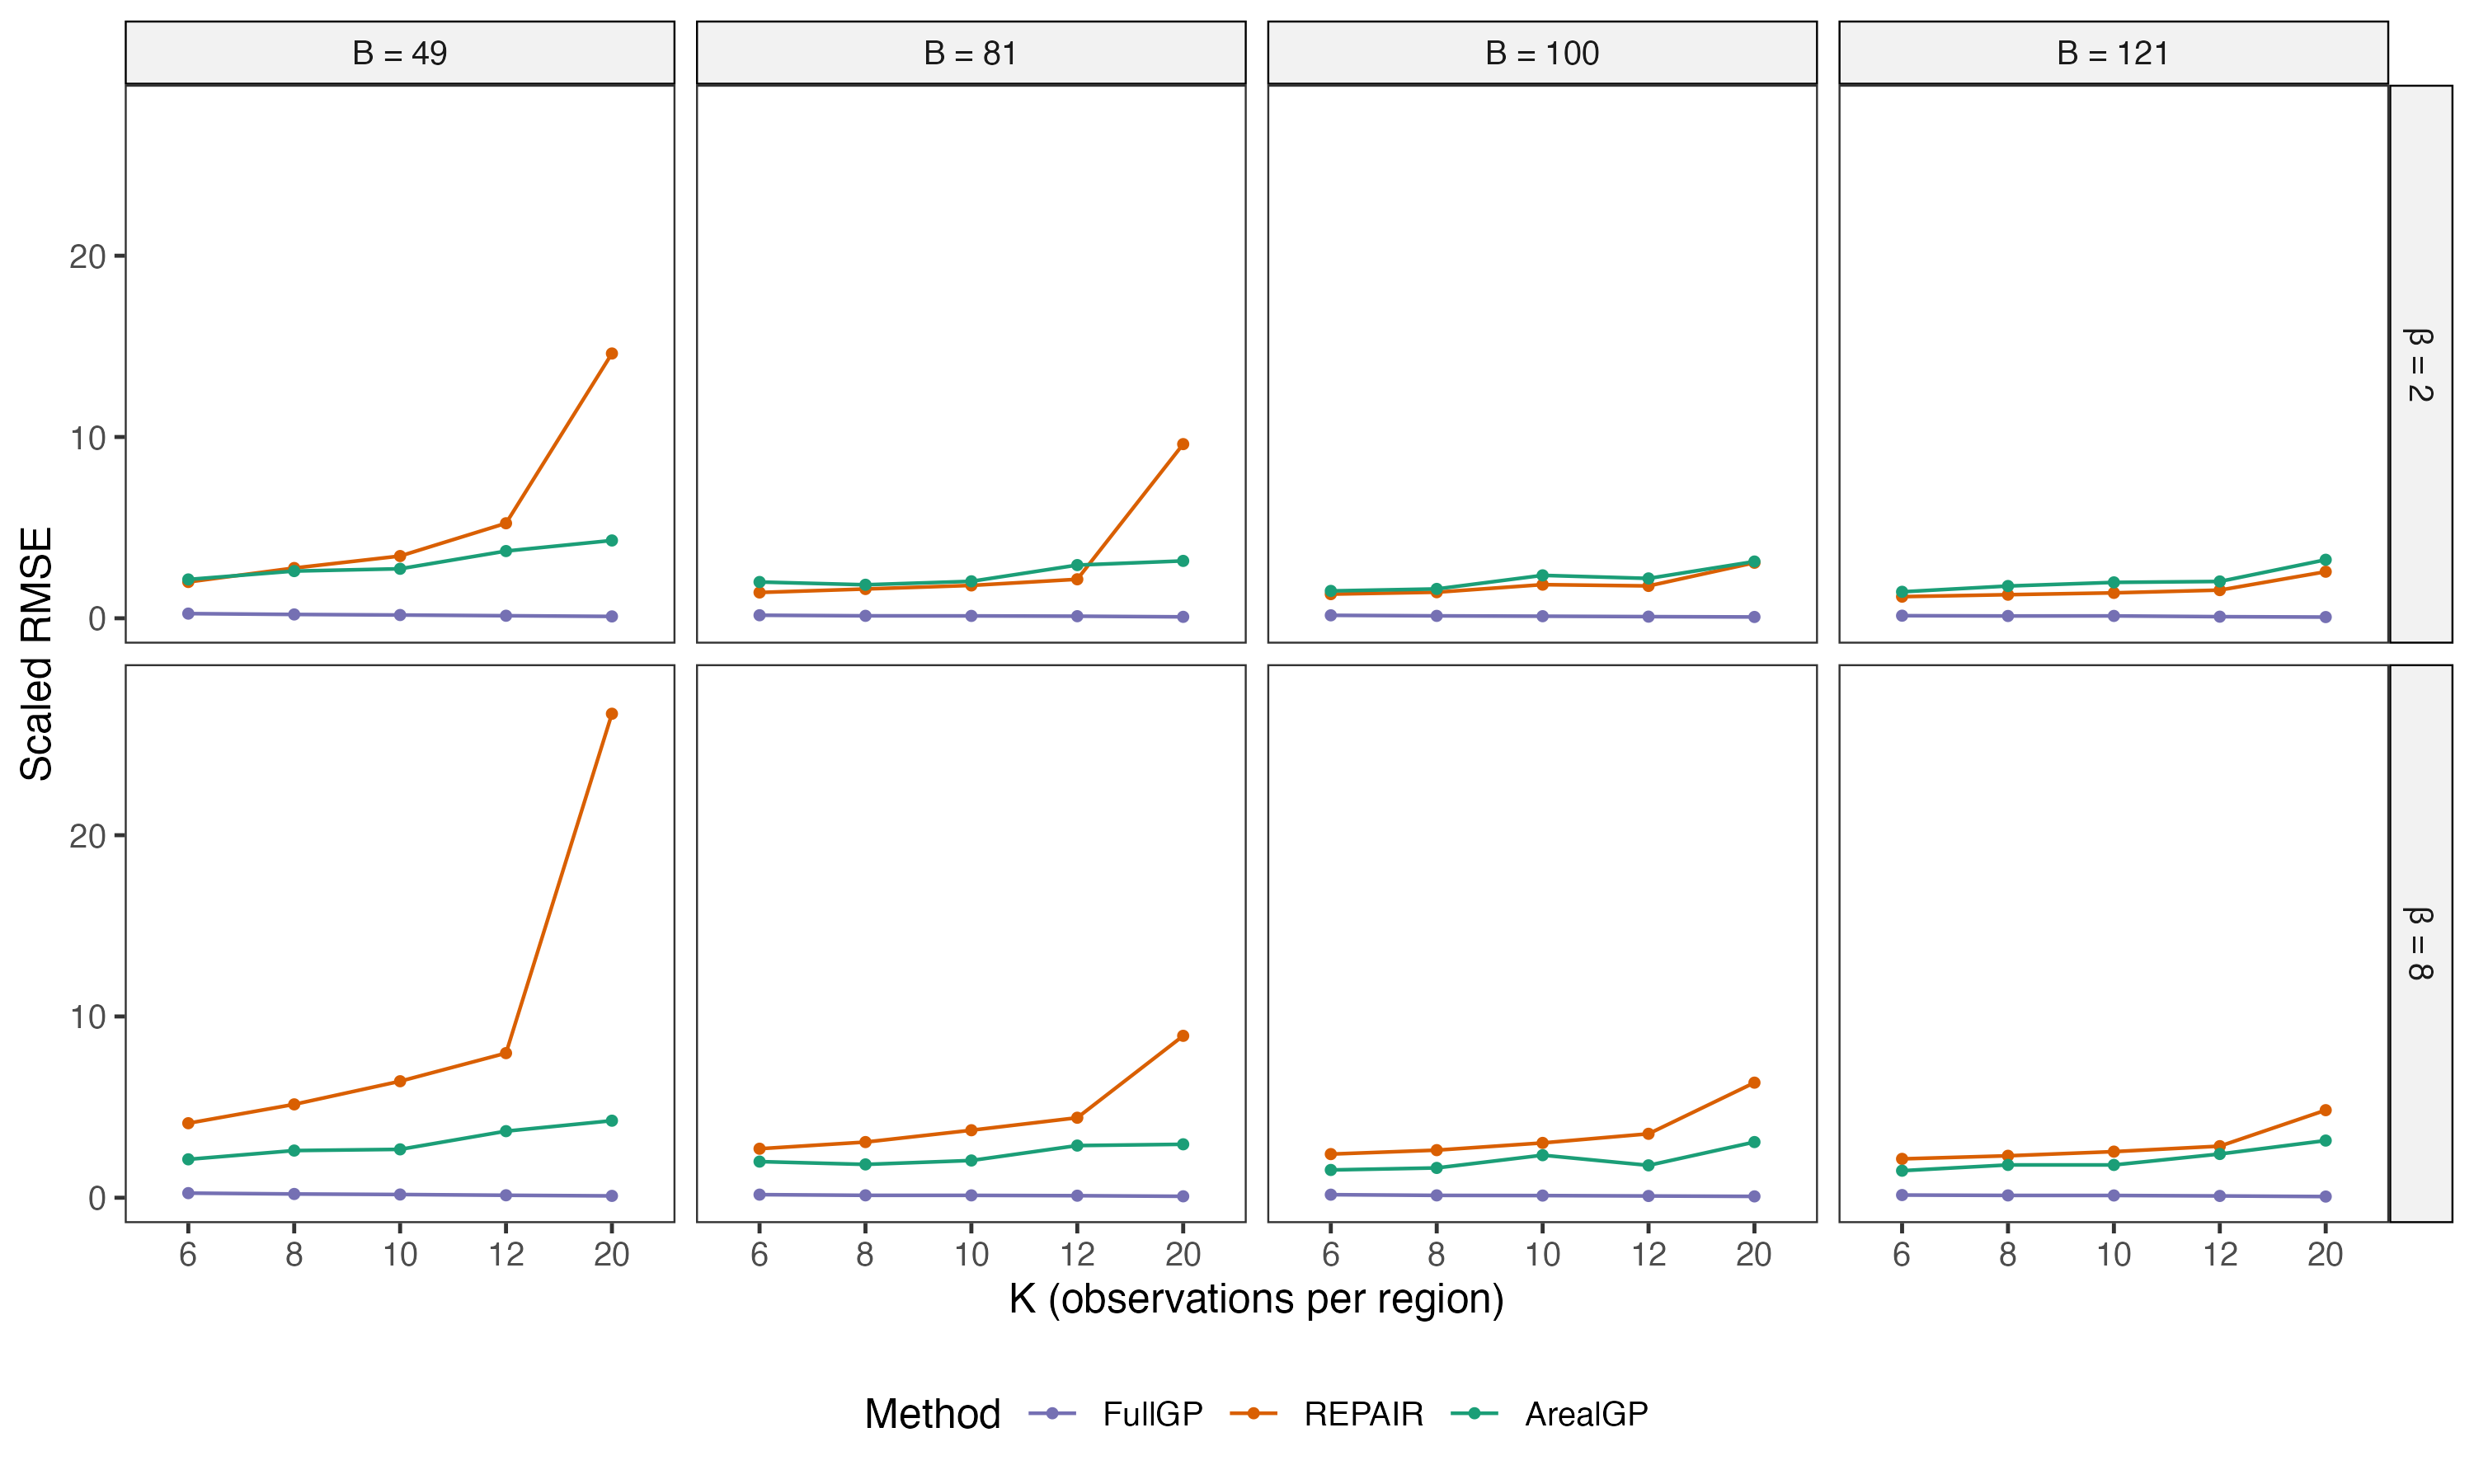
\includegraphics[width=0.9\textwidth]{Figures/lineplot_scaled_rmse_tausq.png}

\medskip
{\footnotesize \textbf{(a)} Scaled RMSE of $\hat{\tau}^2$.}

\medskip
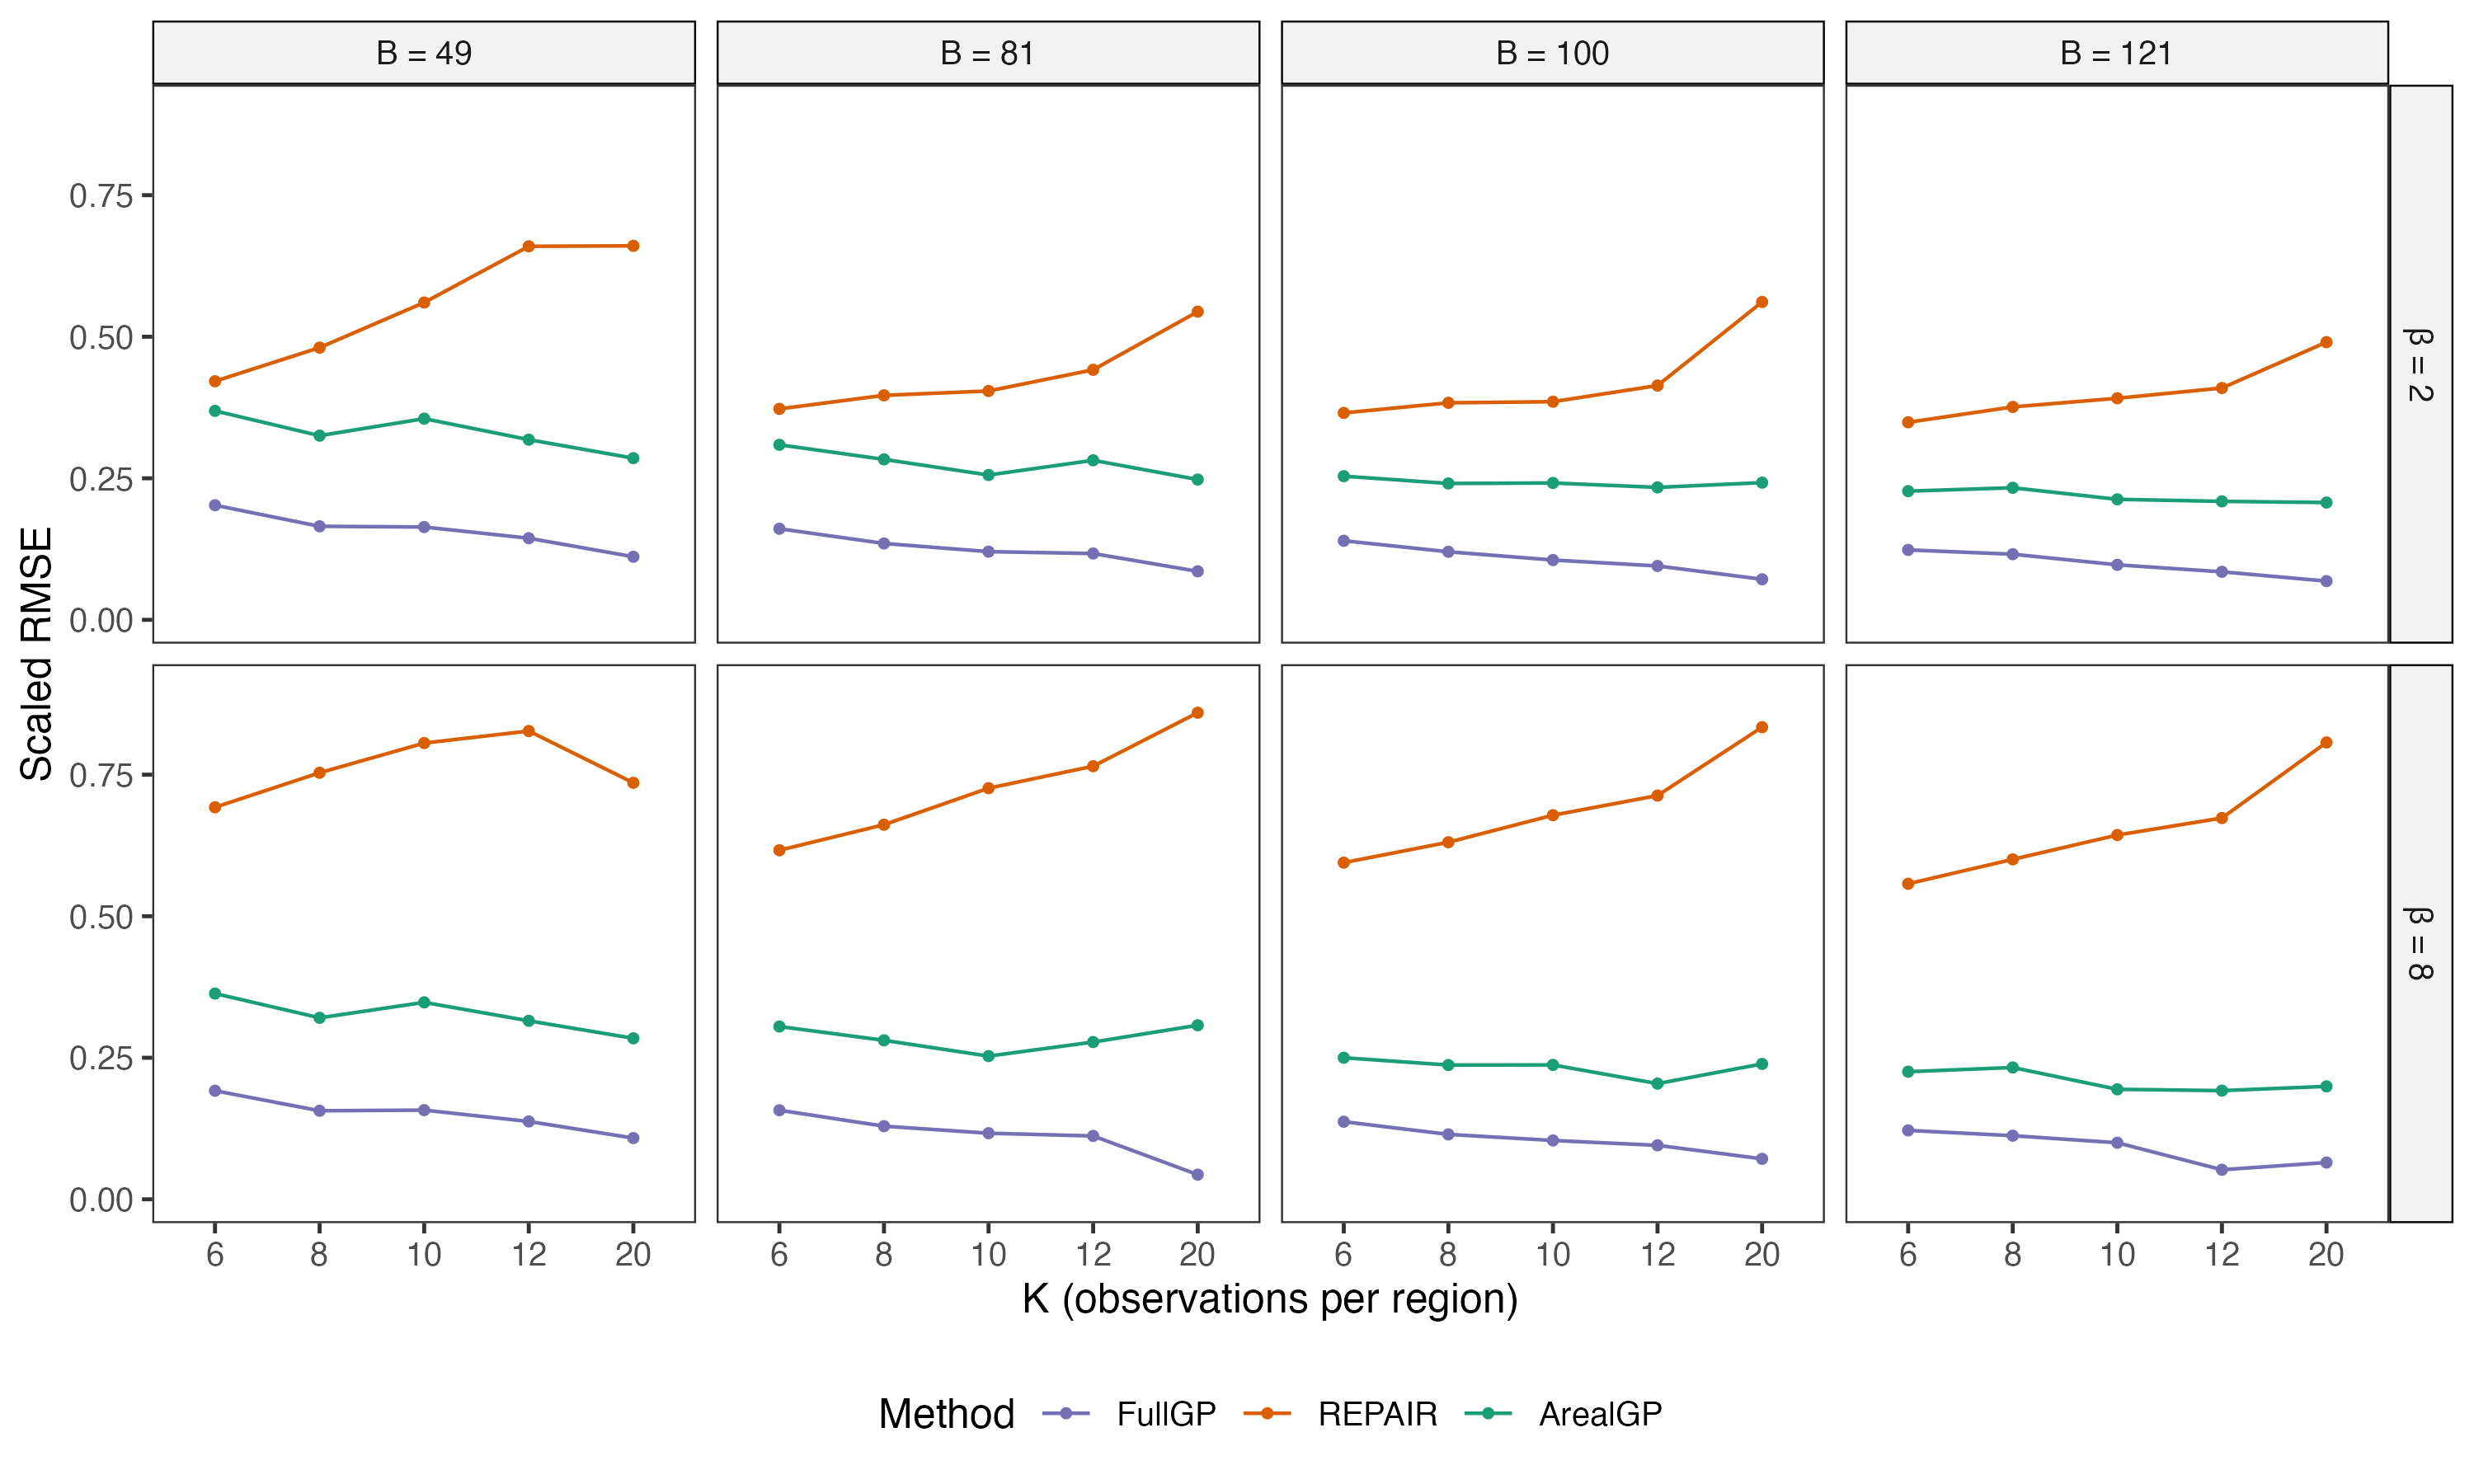
\includegraphics[width=0.9\textwidth]{Figures/lineplot_scaled_rmse_sigmasqphi.png}

\medskip
{\footnotesize \textbf{(b)} Scaled RMSE of $\widehat{\sigma^2 \phi}$.}

\caption{Scaled RMSE plots for the variance-related parameters.}
\label{fig:rmse_lines}
\end{figure}

Estimation of covariance parameters such as $\sigma^2$ and $\phi$ is often challenging in finite samples and this difficulty is reflected in our simulations through the comparatively higher RMSE values for variance-related parameters relative to the regression coefficient. This is consistent with the broader literature: \citet{zhang2004inconsistent} showed that under fixed-domain asymptotics, the variance and range parameters of the Matérn class cannot be estimated consistently in isolation, and only certain microergodic combinations remain well-identified. While this non-identifiability is specific to the fixed-domain regime, it underscores a more general difficulty in disentangling covariance parameters that persists even at moderate sample sizes.

In our setting, the finite-sample imprecision in estimating $\sigma^2$ and $\phi$ is likely further amplified by the latent permutation structure and by the use of a mean-field variational approximation. The mean-field factorization substantially simplifies computation, but it can also reduce accuracy for nuisance covariance parameters, which is consistent with the larger RMSE values observed in our experiments.

\newpage
\section{Simulation Study Details}\label{suppsec:simulation-details}

\subsection*{Data-Generating Process}

For each configuration $(K, B)$, the domain values $\{s_i\}_{i=1}^n$ were generated by partitioning the unit square into a $\sqrt{B} \times \sqrt{B}$ grid and sampling $K$ locations uniformly within each grid cell. The exposure vector was drawn as $X_j \overset{\text{iid}}{\sim} \calN(0,1)$ for $j=1,\ldots,n$. The spatial random effect $\bW \sim \calN_n(\bzero, \bSig^\ast)$ with $\bSig^\ast = \sigma^2 \bR(\phi)$ following an exponential covariance kernel $C(d) = \sigma^2 \exp(-d/\phi)$, with $\sigma^2 = 5$ and range $\phi = 0.5$. The iid noise vector was drawn as $\beps \sim \calN_n(\bzero, \tau^2 \bI_n)$ with $\tau^2 = 0.5$. The outcome was then generated as $\bY = \bPix \bX \beta + \bPis \bW + \beps$, where $\bPi_X = \mathrm{bdiag}(\bpix)$ and $\bPi_S = \mathrm{bdiag}(\bpis)$.

For each $(K,B)$ pair, the within-block Hamming distances $d_H(\bpix, \bI_K)$ and $d_H(\bpis, \bI_K)$ were drawn independently and uniformly from $\{1,\ldots,K\}$ and held fixed across 100 independent replicates. Two signal regimes were considered: $\beta = 2$ (low SNR) and $\beta = 8$ (high SNR).

\subsection*{Hyperparameter Settings for REPAIR}

The REPAIR algorithm was initialised with $\kappa_X^{(0)} = \kappa_S^{(0)} = 1.0$, minimum temperature $\kappa_{\min} = 0.05$, exponential decay rate $\alpha = 0.95$, and learning rates $l_X = l_S = 0.01$. The prior on $\beta$ was $\calN(0, 100)$ and the priors on $\sigma^2$ and $\tau^2$ were weakly informative Inverse-Gamma$(0.01, 0.01)$. Convergence was declared when the relative change in the ELBO fell below $\epsilon = 10^{-4}$.

\subsection*{Methods}

Three estimators were compared on each simulated dataset. \textbf{FullGP} treats the true permutation matrices $(\bPix, \bPis)$ as known and fits a standard spatial GP regression by maximum likelihood, serving as an oracle benchmark. \textbf{ArealGP} aggregates both exposure and outcome to the block level and applies GLS with an exponential kernel; this is a natural competitor that ignores within-block permutation structure. \textbf{REPAIR} is the proposed variational Bayes estimator from Algorithms~\ref{alg-parameter-est}--\ref{alg:perm-est}. For FullGP and ArealGP, MLE was computed via numerical optimisation.

\begin{figure}[!htbp]
\centering
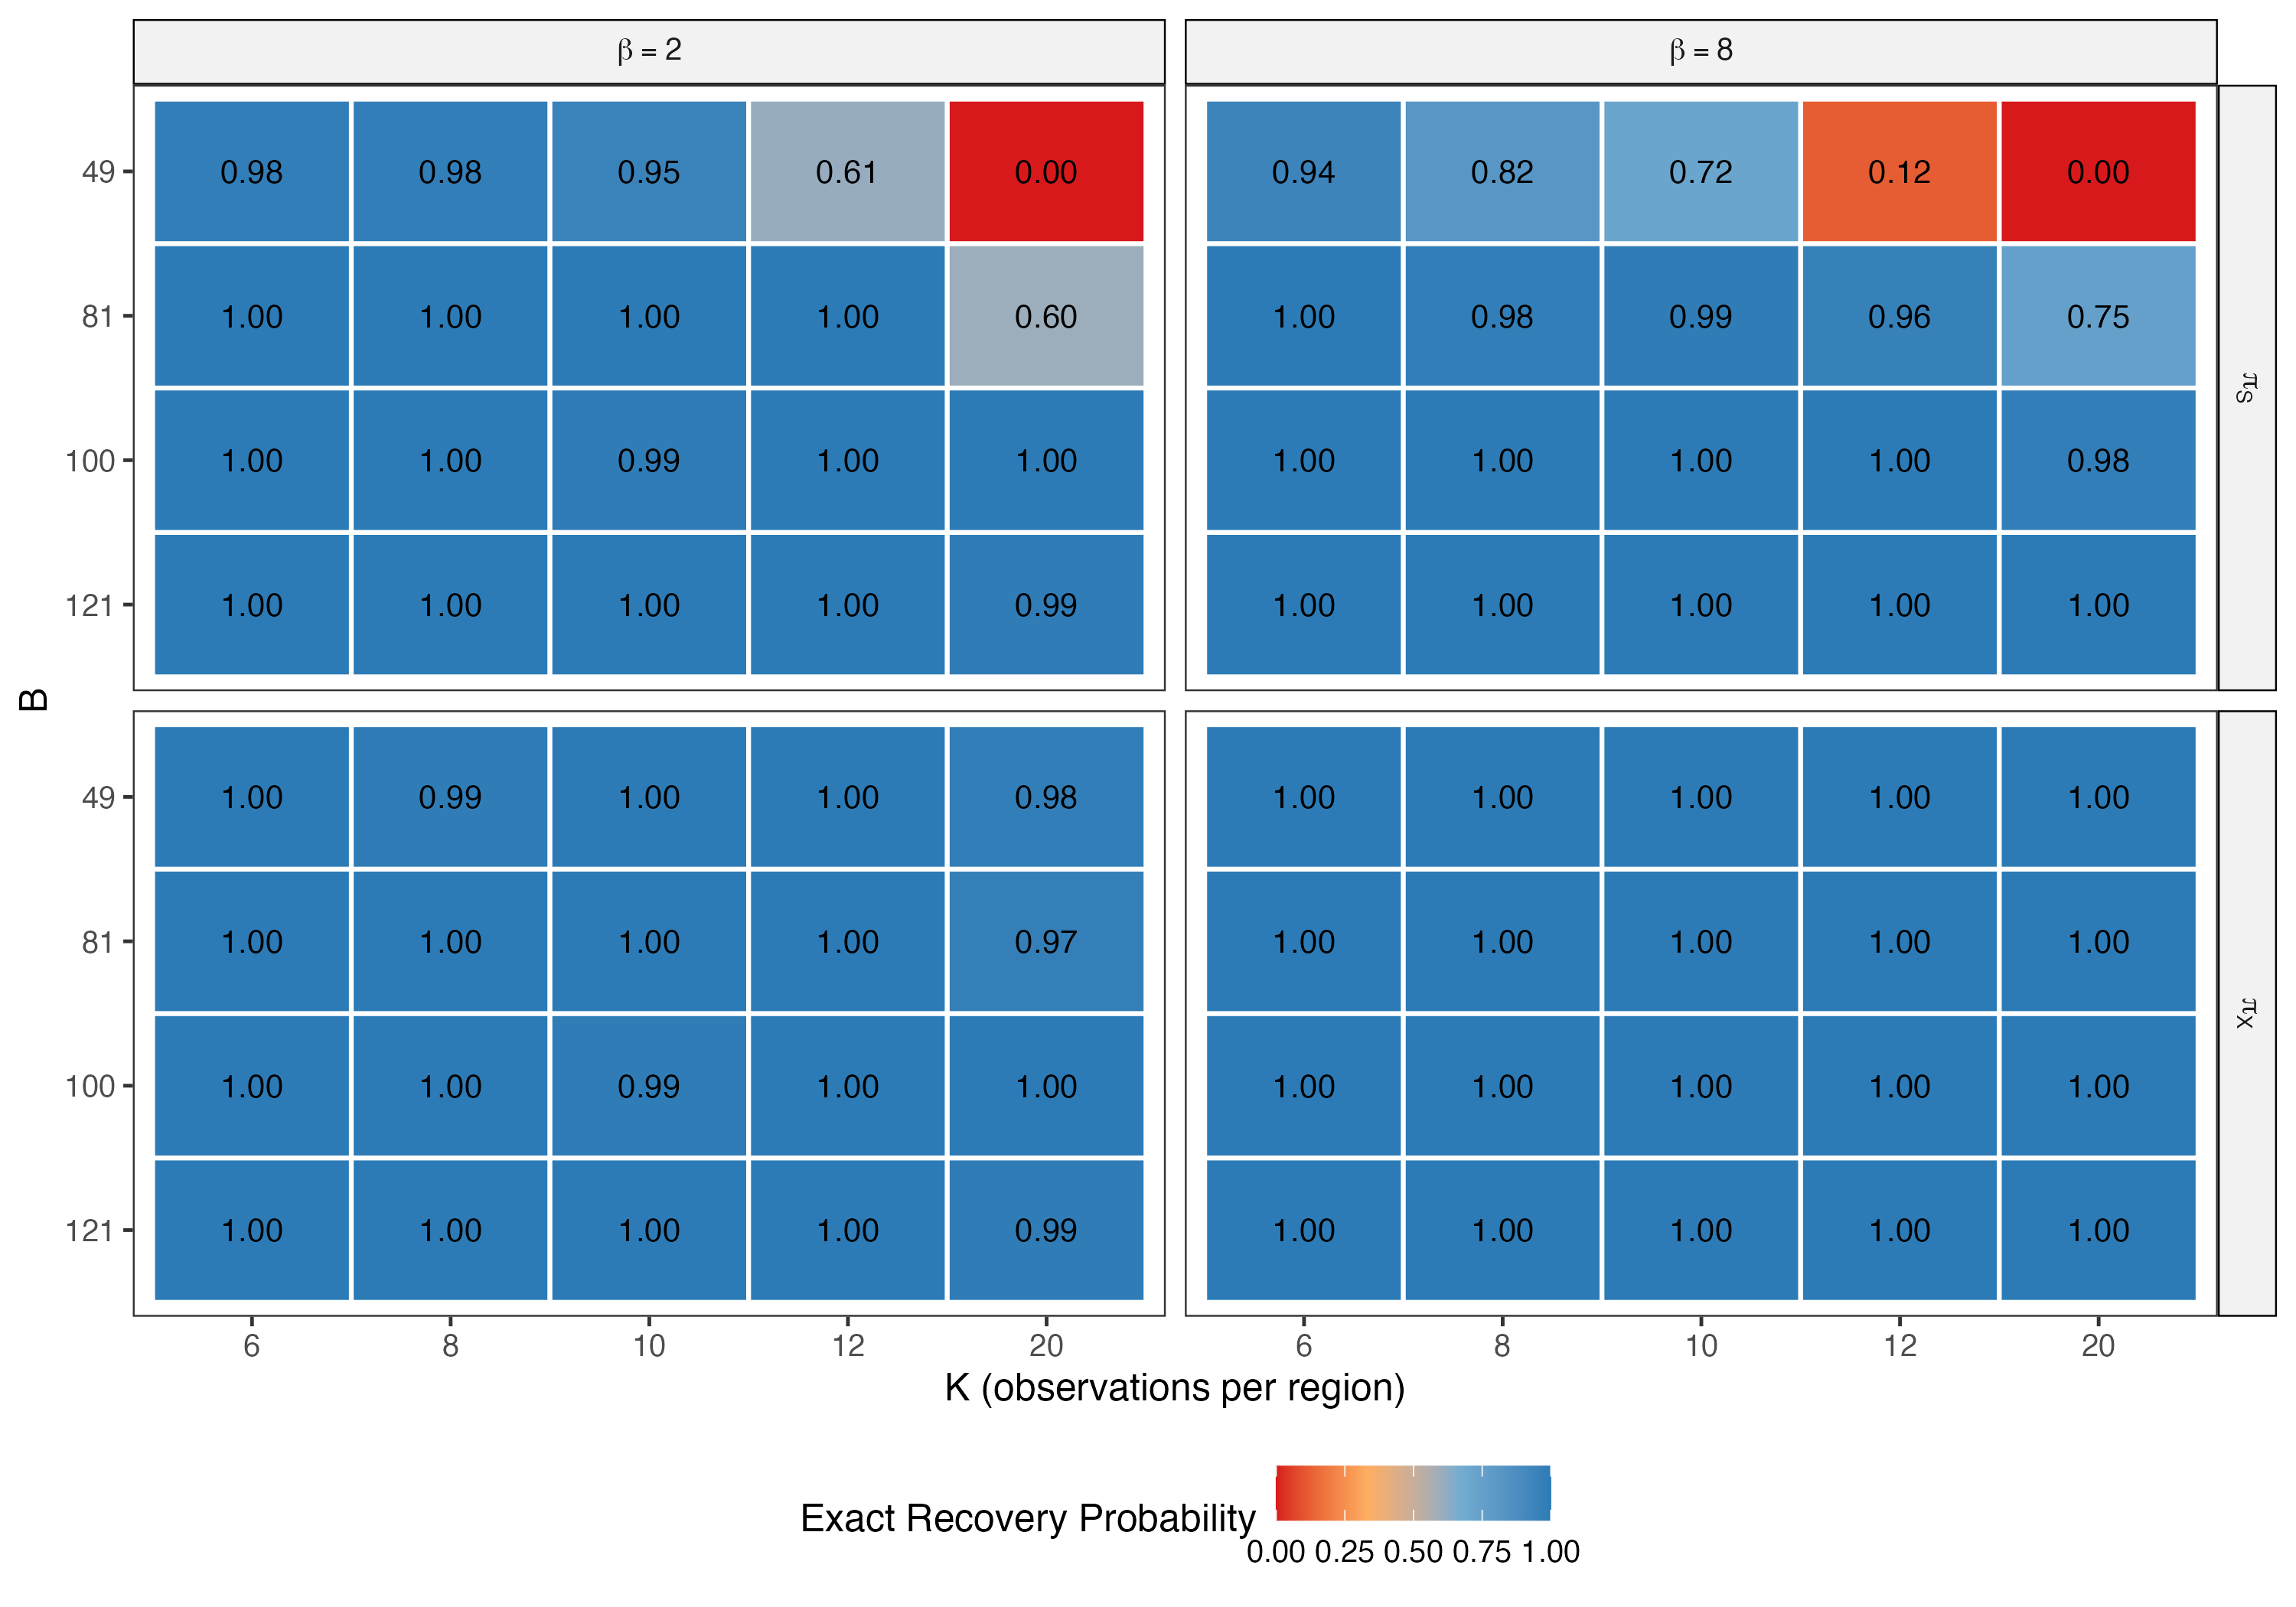
\includegraphics[width=0.9\textwidth]{Figures/perm_recovery_combined_exact.png}
\caption{Permutation recovery performance of the REPAIR method across simulation settings.
Cells show the estimated recovery probability for the permutation matrices $\bpis$ and $\bpix$
across different values of the number of blocks $B$ and observations per block $K$,
under two signal regimes ($\beta = 2$ and $\beta = 8$).}
\label{fig:perm_recovery}
\end{figure}

% \newpage
\section{Meuse Dataset: Background and Preprocessing}\label{suppsec:data-details}

\subsection*{Dataset Background}

The Meuse dataset \citep{pebesma2012package} records the concentrations of four heavy metals --- cadmium (Cd), copper (Cu), lead (Pb), and zinc (Zn) --- at 155 locations on the floodplain of the river Meuse near the village of Stein, the Netherlands, together with several landscape covariates including elevation, distance to the river, and flood frequency class. A distinguishing feature of this dataset is the presence of the river Meuse itself as a naturally occurring geographic boundary that induces substantial spatial heterogeneity: metal concentrations are generally higher in lower-lying areas near the riverbank and decrease monotonically with elevation. The floodplain soils are used for agriculture, making the characterisation of heavy metal distributions of direct environmental and public health interest.

\subsection*{Variable Selection and Preprocessing}

We focus on zinc concentration as the outcome, motivated by its strong spatial gradient and its status as the most abundant heavy metal in this dataset. Elevation is used as the exposure, as it is the primary landscape variable explaining the spatial distribution of zinc. The transformed response $Y = \log(1 + \text{zinc})$ was used to reduce skewness. Both the exposure and the transformed outcome were centred to have mean zero, and the spatial coordinates were rescaled to the unit square for numerical stability in kernel computations.

\subsection*{Construction of the Doubly-Unlinked Dataset}

From the original $n = 155$ observations, five were removed at random to give $n = 150$, enabling a clean partition into equal-sized contiguous blocks. Locations were ordered by the first spatial coordinate (longitude), then divided into non-overlapping contiguous blocks. Within each block, the exposure values and spatial coordinates were independently permuted, thereby breaking both the covariate--response link and the response--domain link and inducing the doubly-unlinked structure. Two blocking schemes were considered: (a) $B = 15$ blocks of size $K = 10$, and (b) $B = 30$ blocks of size $K = 5$. The coarser partition has fewer, larger blocks, making within-block permutation recovery harder; the finer partition has smaller blocks, facilitating recovery but providing less spatial averaging.

\bibliographystyle{abbrvnat}
\bibliography{doubly_unlinked}
\end{document}